\documentclass[twoside]{book}

% Packages required by doxygen
\usepackage{fixltx2e}
\usepackage{calc}
\usepackage{doxygen}
\usepackage[export]{adjustbox} % also loads graphicx
\usepackage{graphicx}
\usepackage[utf8]{inputenc}
\usepackage{makeidx}
\usepackage{multicol}
\usepackage{multirow}
\PassOptionsToPackage{warn}{textcomp}
\usepackage{textcomp}
\usepackage[nointegrals]{wasysym}
\usepackage[table]{xcolor}

% Font selection
\usepackage[T1]{fontenc}
\usepackage[scaled=.90]{helvet}
\usepackage{courier}
\usepackage{amssymb}
\usepackage{sectsty}
\renewcommand{\familydefault}{\sfdefault}
\allsectionsfont{%
  \fontseries{bc}\selectfont%
  \color{darkgray}%
}
\renewcommand{\DoxyLabelFont}{%
  \fontseries{bc}\selectfont%
  \color{darkgray}%
}
\newcommand{\+}{\discretionary{\mbox{\scriptsize$\hookleftarrow$}}{}{}}

% Page & text layout
\usepackage{geometry}
\geometry{%
  a4paper,%
  top=2.5cm,%
  bottom=2.5cm,%
  left=2.5cm,%
  right=2.5cm%
}
\tolerance=750
\hfuzz=15pt
\hbadness=750
\setlength{\emergencystretch}{15pt}
\setlength{\parindent}{0cm}
\setlength{\parskip}{3ex plus 2ex minus 2ex}
\makeatletter
\renewcommand{\paragraph}{%
  \@startsection{paragraph}{4}{0ex}{-1.0ex}{1.0ex}{%
    \normalfont\normalsize\bfseries\SS@parafont%
  }%
}
\renewcommand{\subparagraph}{%
  \@startsection{subparagraph}{5}{0ex}{-1.0ex}{1.0ex}{%
    \normalfont\normalsize\bfseries\SS@subparafont%
  }%
}
\makeatother

% Headers & footers
\usepackage{fancyhdr}
\pagestyle{fancyplain}
\fancyhead[LE]{\fancyplain{}{\bfseries\thepage}}
\fancyhead[CE]{\fancyplain{}{}}
\fancyhead[RE]{\fancyplain{}{\bfseries\leftmark}}
\fancyhead[LO]{\fancyplain{}{\bfseries\rightmark}}
\fancyhead[CO]{\fancyplain{}{}}
\fancyhead[RO]{\fancyplain{}{\bfseries\thepage}}
\fancyfoot[LE]{\fancyplain{}{}}
\fancyfoot[CE]{\fancyplain{}{}}
\fancyfoot[RE]{\fancyplain{}{\bfseries\scriptsize Generated by Doxygen }}
\fancyfoot[LO]{\fancyplain{}{\bfseries\scriptsize Generated by Doxygen }}
\fancyfoot[CO]{\fancyplain{}{}}
\fancyfoot[RO]{\fancyplain{}{}}
\renewcommand{\footrulewidth}{0.4pt}
\renewcommand{\chaptermark}[1]{%
  \markboth{#1}{}%
}
\renewcommand{\sectionmark}[1]{%
  \markright{\thesection\ #1}%
}

% Indices & bibliography
\usepackage{natbib}
\usepackage[titles]{tocloft}
\setcounter{tocdepth}{3}
\setcounter{secnumdepth}{5}
\makeindex

% Hyperlinks (required, but should be loaded last)
\usepackage{ifpdf}
\ifpdf
  \usepackage[pdftex,pagebackref=true]{hyperref}
\else
  \usepackage[ps2pdf,pagebackref=true]{hyperref}
\fi
\hypersetup{%
  colorlinks=true,%
  linkcolor=blue,%
  citecolor=blue,%
  unicode%
}

% Custom commands
\newcommand{\clearemptydoublepage}{%
  \newpage{\pagestyle{empty}\cleardoublepage}%
}

\usepackage{caption}
\captionsetup{labelsep=space,justification=centering,font={bf},singlelinecheck=off,skip=4pt,position=top}

%===== C O N T E N T S =====

\begin{document}

% Titlepage & ToC
\hypersetup{pageanchor=false,
             bookmarksnumbered=true,
             pdfencoding=unicode
            }
\pagenumbering{alph}
\begin{titlepage}
\vspace*{7cm}
\begin{center}%
{\Large Hellfire\+OS v2.0 }\\
\vspace*{1cm}
{\large Generated by Doxygen 1.8.13}\\
\end{center}
\end{titlepage}
\clearemptydoublepage
\pagenumbering{roman}
\tableofcontents
\clearemptydoublepage
\pagenumbering{arabic}
\hypersetup{pageanchor=true}

%--- Begin generated contents ---
\chapter{Data Structure Index}
\section{Data Structures}
Here are the data structures with brief descriptions\+:\begin{DoxyCompactList}
\item\contentsline{section}{\hyperlink{structarp__entry}{arp\+\_\+entry} }{\pageref{structarp__entry}}{}
\item\contentsline{section}{\hyperlink{structcondvar}{condvar} \\*Condition variable data structure }{\pageref{structcondvar}}{}
\item\contentsline{section}{\hyperlink{structlist}{list} \\*List data structure }{\pageref{structlist}}{}
\item\contentsline{section}{\hyperlink{structmem__block}{mem\+\_\+block} }{\pageref{structmem__block}}{}
\item\contentsline{section}{\hyperlink{structmem__chunk}{mem\+\_\+chunk} }{\pageref{structmem__chunk}}{}
\item\contentsline{section}{\hyperlink{structmem__chunk__ptr}{mem\+\_\+chunk\+\_\+ptr} }{\pageref{structmem__chunk__ptr}}{}
\item\contentsline{section}{\hyperlink{unionmem__header__union}{mem\+\_\+header\+\_\+union} }{\pageref{unionmem__header__union}}{}
\item\contentsline{section}{\hyperlink{structmtx}{mtx} \\*Mutex data structure }{\pageref{structmtx}}{}
\item\contentsline{section}{\hyperlink{structpcb__entry}{pcb\+\_\+entry} }{\pageref{structpcb__entry}}{}
\item\contentsline{section}{\hyperlink{structqueue}{queue} \\*Queue data structure }{\pageref{structqueue}}{}
\item\contentsline{section}{\hyperlink{structsem}{sem} \\*Semaphore data structure }{\pageref{structsem}}{}
\item\contentsline{section}{\hyperlink{structtcb__entry}{tcb\+\_\+entry} \\*Task control block (T\+CB) and processor control block (P\+CB) entry data structures }{\pageref{structtcb__entry}}{}
\item\contentsline{section}{\hyperlink{structuudp}{uudp} }{\pageref{structuudp}}{}
\end{DoxyCompactList}

\chapter{File Index}
\section{File List}
Here is a list of all files with brief descriptions\+:\begin{DoxyCompactList}
\item\contentsline{section}{drivers/noc/\hyperlink{ni__hermes_8c}{ni\+\_\+hermes.\+c} }{\pageref{ni__hermes_8c}}{}
\item\contentsline{section}{drivers/noc/\hyperlink{noc_8c}{noc.\+c} }{\pageref{noc_8c}}{}
\item\contentsline{section}{drivers/noc/\hyperlink{noc__rpc_8c}{noc\+\_\+rpc.\+c} }{\pageref{noc__rpc_8c}}{}
\item\contentsline{section}{drivers/noc/include/\hyperlink{ni__generic_8h}{ni\+\_\+generic.\+h} }{\pageref{ni__generic_8h}}{}
\item\contentsline{section}{drivers/noc/include/\hyperlink{noc_8h}{noc.\+h} }{\pageref{noc_8h}}{}
\item\contentsline{section}{drivers/noc/include/\hyperlink{noc__rpc_8h}{noc\+\_\+rpc.\+h} }{\pageref{noc__rpc_8h}}{}
\item\contentsline{section}{net/include/\hyperlink{ustack_8h}{ustack.\+h} }{\pageref{ustack_8h}}{}
\item\contentsline{section}{net/include/\hyperlink{uudp_8h}{uudp.\+h} }{\pageref{uudp_8h}}{}
\item\contentsline{section}{net/uudp/\hyperlink{uudp_8c}{uudp.\+c} }{\pageref{uudp_8c}}{}
\item\contentsline{section}{sys/include/\hyperlink{condvar_8h}{condvar.\+h} }{\pageref{condvar_8h}}{}
\item\contentsline{section}{sys/include/\hyperlink{ecodes_8h}{ecodes.\+h} }{\pageref{ecodes_8h}}{}
\item\contentsline{section}{sys/include/\hyperlink{hellfire_8h}{hellfire.\+h} }{\pageref{hellfire_8h}}{}
\item\contentsline{section}{sys/include/\hyperlink{kernel_8h}{kernel.\+h} }{\pageref{kernel_8h}}{}
\item\contentsline{section}{sys/include/\hyperlink{kprintf_8h}{kprintf.\+h} }{\pageref{kprintf_8h}}{}
\item\contentsline{section}{sys/include/\hyperlink{list_8h}{list.\+h} }{\pageref{list_8h}}{}
\item\contentsline{section}{sys/include/\hyperlink{main_8h}{main.\+h} }{\pageref{main_8h}}{}
\item\contentsline{section}{sys/include/\hyperlink{malloc_8h}{malloc.\+h} }{\pageref{malloc_8h}}{}
\item\contentsline{section}{sys/include/\hyperlink{mutex_8h}{mutex.\+h} }{\pageref{mutex_8h}}{}
\item\contentsline{section}{sys/include/\hyperlink{panic_8h}{panic.\+h} }{\pageref{panic_8h}}{}
\item\contentsline{section}{sys/include/\hyperlink{processor_8h}{processor.\+h} }{\pageref{processor_8h}}{}
\item\contentsline{section}{sys/include/\hyperlink{queue_8h}{queue.\+h} }{\pageref{queue_8h}}{}
\item\contentsline{section}{sys/include/\hyperlink{scheduler_8h}{scheduler.\+h} }{\pageref{scheduler_8h}}{}
\item\contentsline{section}{sys/include/\hyperlink{semaphore_8h}{semaphore.\+h} }{\pageref{semaphore_8h}}{}
\item\contentsline{section}{sys/include/\hyperlink{task_8h}{task.\+h} }{\pageref{task_8h}}{}
\item\contentsline{section}{sys/kernel/\hyperlink{main_8c}{main.\+c} }{\pageref{main_8c}}{}
\item\contentsline{section}{sys/kernel/\hyperlink{panic_8c}{panic.\+c} }{\pageref{panic_8c}}{}
\item\contentsline{section}{sys/kernel/\hyperlink{processor_8c}{processor.\+c} }{\pageref{processor_8c}}{}
\item\contentsline{section}{sys/kernel/\hyperlink{scheduler_8c}{scheduler.\+c} }{\pageref{scheduler_8c}}{}
\item\contentsline{section}{sys/kernel/\hyperlink{task_8c}{task.\+c} }{\pageref{task_8c}}{}
\item\contentsline{section}{sys/lib/\hyperlink{kprintf_8c}{kprintf.\+c} }{\pageref{kprintf_8c}}{}
\item\contentsline{section}{sys/lib/\hyperlink{list_8c}{list.\+c} }{\pageref{list_8c}}{}
\item\contentsline{section}{sys/lib/\hyperlink{malloc_8c}{malloc.\+c} }{\pageref{malloc_8c}}{}
\item\contentsline{section}{sys/lib/\hyperlink{queue_8c}{queue.\+c} }{\pageref{queue_8c}}{}
\item\contentsline{section}{sys/sync/\hyperlink{condvar_8c}{condvar.\+c} }{\pageref{condvar_8c}}{}
\item\contentsline{section}{sys/sync/\hyperlink{mutex_8c}{mutex.\+c} }{\pageref{mutex_8c}}{}
\item\contentsline{section}{sys/sync/\hyperlink{semaphore_8c}{semaphore.\+c} }{\pageref{semaphore_8c}}{}
\end{DoxyCompactList}

\chapter{Data Structure Documentation}
\hypertarget{structarp__entry}{}\section{arp\+\_\+entry Struct Reference}
\label{structarp__entry}\index{arp\+\_\+entry@{arp\+\_\+entry}}


{\ttfamily \#include $<$ustack.\+h$>$}

\subsection*{Data Fields}
\begin{DoxyCompactItemize}
\item 
uint8\+\_\+t \hyperlink{structarp__entry_a66483dc0b1c1ef9215b1e85185044d54}{ip} \mbox{[}4\mbox{]}
\item 
uint8\+\_\+t \hyperlink{structarp__entry_af9a7c3845ffe5ef927c4d94b65d9cb7e}{mac} \mbox{[}6\mbox{]}
\end{DoxyCompactItemize}


\subsection{Field Documentation}
\mbox{\Hypertarget{structarp__entry_a66483dc0b1c1ef9215b1e85185044d54}\label{structarp__entry_a66483dc0b1c1ef9215b1e85185044d54}} 
\index{arp\+\_\+entry@{arp\+\_\+entry}!ip@{ip}}
\index{ip@{ip}!arp\+\_\+entry@{arp\+\_\+entry}}
\subsubsection{\texorpdfstring{ip}{ip}}
{\footnotesize\ttfamily uint8\+\_\+t arp\+\_\+entry\+::ip\mbox{[}4\mbox{]}}

\mbox{\Hypertarget{structarp__entry_af9a7c3845ffe5ef927c4d94b65d9cb7e}\label{structarp__entry_af9a7c3845ffe5ef927c4d94b65d9cb7e}} 
\index{arp\+\_\+entry@{arp\+\_\+entry}!mac@{mac}}
\index{mac@{mac}!arp\+\_\+entry@{arp\+\_\+entry}}
\subsubsection{\texorpdfstring{mac}{mac}}
{\footnotesize\ttfamily uint8\+\_\+t arp\+\_\+entry\+::mac\mbox{[}6\mbox{]}}



The documentation for this struct was generated from the following file\+:\begin{DoxyCompactItemize}
\item 
net/include/\hyperlink{ustack_8h}{ustack.\+h}\end{DoxyCompactItemize}

\hypertarget{structcondvar}{}\section{condvar Struct Reference}
\label{structcondvar}\index{condvar@{condvar}}


Condition variable data structure.  




{\ttfamily \#include $<$condvar.\+h$>$}



Collaboration diagram for condvar\+:\nopagebreak
\begin{figure}[H]
\begin{center}
\leavevmode
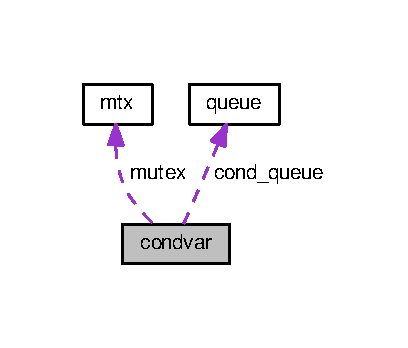
\includegraphics[width=196pt]{structcondvar__coll__graph}
\end{center}
\end{figure}
\subsection*{Data Fields}
\begin{DoxyCompactItemize}
\item 
struct \hyperlink{structqueue}{queue} $\ast$ \hyperlink{structcondvar_abf91dd97763d95af19ee92a17f55afb8}{cond\+\_\+queue}
\item 
\hyperlink{mutex_8h_af6ff4e9d708d58c0662f63a81713a926}{mutex\+\_\+t} \hyperlink{structcondvar_a573f1b5d528d692d581b734913807b66}{mutex}
\end{DoxyCompactItemize}


\subsection{Detailed Description}
Condition variable data structure. 

\subsection{Field Documentation}
\mbox{\Hypertarget{structcondvar_abf91dd97763d95af19ee92a17f55afb8}\label{structcondvar_abf91dd97763d95af19ee92a17f55afb8}} 
\index{condvar@{condvar}!cond\+\_\+queue@{cond\+\_\+queue}}
\index{cond\+\_\+queue@{cond\+\_\+queue}!condvar@{condvar}}
\subsubsection{\texorpdfstring{cond\+\_\+queue}{cond\_queue}}
{\footnotesize\ttfamily struct \hyperlink{structqueue}{queue}$\ast$ condvar\+::cond\+\_\+queue}

queue for tasks waiting on the condition variable \mbox{\Hypertarget{structcondvar_a573f1b5d528d692d581b734913807b66}\label{structcondvar_a573f1b5d528d692d581b734913807b66}} 
\index{condvar@{condvar}!mutex@{mutex}}
\index{mutex@{mutex}!condvar@{condvar}}
\subsubsection{\texorpdfstring{mutex}{mutex}}
{\footnotesize\ttfamily \hyperlink{mutex_8h_af6ff4e9d708d58c0662f63a81713a926}{mutex\+\_\+t} condvar\+::mutex}

mutex used for the critical section associated with the condition variable 

The documentation for this struct was generated from the following file\+:\begin{DoxyCompactItemize}
\item 
sys/include/\hyperlink{condvar_8h}{condvar.\+h}\end{DoxyCompactItemize}

\hypertarget{structlist}{}\section{list Struct Reference}
\label{structlist}\index{list@{list}}


List data structure.  




{\ttfamily \#include $<$list.\+h$>$}



Collaboration diagram for list\+:\nopagebreak
\begin{figure}[H]
\begin{center}
\leavevmode
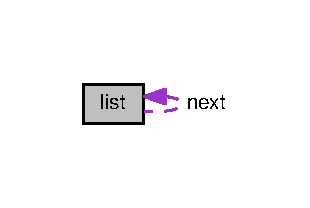
\includegraphics[width=149pt]{structlist__coll__graph}
\end{center}
\end{figure}
\subsection*{Data Fields}
\begin{DoxyCompactItemize}
\item 
void $\ast$ \hyperlink{structlist_af3f79a2886a3f27cdfdfa202c2affc68}{elem}
\item 
struct \hyperlink{structlist}{list} $\ast$ \hyperlink{structlist_a1900fe79e875e2838625b2eb60837f8f}{next}
\end{DoxyCompactItemize}


\subsection{Detailed Description}
List data structure. 

\subsection{Field Documentation}
\mbox{\Hypertarget{structlist_af3f79a2886a3f27cdfdfa202c2affc68}\label{structlist_af3f79a2886a3f27cdfdfa202c2affc68}} 
\index{list@{list}!elem@{elem}}
\index{elem@{elem}!list@{list}}
\subsubsection{\texorpdfstring{elem}{elem}}
{\footnotesize\ttfamily void$\ast$ list\+::elem}

pointer to list node data \mbox{\Hypertarget{structlist_a1900fe79e875e2838625b2eb60837f8f}\label{structlist_a1900fe79e875e2838625b2eb60837f8f}} 
\index{list@{list}!next@{next}}
\index{next@{next}!list@{list}}
\subsubsection{\texorpdfstring{next}{next}}
{\footnotesize\ttfamily struct \hyperlink{structlist}{list}$\ast$ list\+::next}

pointer to the next list node 

The documentation for this struct was generated from the following file\+:\begin{DoxyCompactItemize}
\item 
sys/include/\hyperlink{list_8h}{list.\+h}\end{DoxyCompactItemize}

\hypertarget{structmem__block}{}\section{mem\+\_\+block Struct Reference}
\label{structmem__block}\index{mem\+\_\+block@{mem\+\_\+block}}


{\ttfamily \#include $<$malloc.\+h$>$}



Collaboration diagram for mem\+\_\+block\+:\nopagebreak
\begin{figure}[H]
\begin{center}
\leavevmode
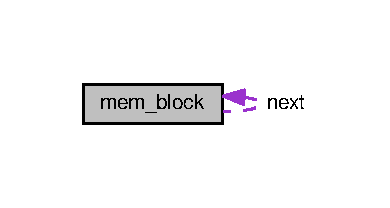
\includegraphics[width=187pt]{structmem__block__coll__graph}
\end{center}
\end{figure}
\subsection*{Data Fields}
\begin{DoxyCompactItemize}
\item 
struct \hyperlink{structmem__block}{mem\+\_\+block} $\ast$ \hyperlink{structmem__block_ac3317f1b6603856e265b1ba15c4a99b8}{next}
\item 
size\+\_\+t \hyperlink{structmem__block_a5ff4ee5dcd970bbc4951eb108c5eec4b}{size}
\end{DoxyCompactItemize}


\subsection{Field Documentation}
\mbox{\Hypertarget{structmem__block_ac3317f1b6603856e265b1ba15c4a99b8}\label{structmem__block_ac3317f1b6603856e265b1ba15c4a99b8}} 
\index{mem\+\_\+block@{mem\+\_\+block}!next@{next}}
\index{next@{next}!mem\+\_\+block@{mem\+\_\+block}}
\subsubsection{\texorpdfstring{next}{next}}
{\footnotesize\ttfamily struct \hyperlink{structmem__block}{mem\+\_\+block} $\ast$ mem\+\_\+block\+::next}

\mbox{\Hypertarget{structmem__block_a5ff4ee5dcd970bbc4951eb108c5eec4b}\label{structmem__block_a5ff4ee5dcd970bbc4951eb108c5eec4b}} 
\index{mem\+\_\+block@{mem\+\_\+block}!size@{size}}
\index{size@{size}!mem\+\_\+block@{mem\+\_\+block}}
\subsubsection{\texorpdfstring{size}{size}}
{\footnotesize\ttfamily size\+\_\+t mem\+\_\+block\+::size}



The documentation for this struct was generated from the following file\+:\begin{DoxyCompactItemize}
\item 
sys/include/\hyperlink{malloc_8h}{malloc.\+h}\end{DoxyCompactItemize}

\hypertarget{structmem__chunk}{}\section{mem\+\_\+chunk Struct Reference}
\label{structmem__chunk}\index{mem\+\_\+chunk@{mem\+\_\+chunk}}


{\ttfamily \#include $<$malloc.\+h$>$}

\subsection*{Data Fields}
\begin{DoxyCompactItemize}
\item 
uint32\+\_\+t \hyperlink{structmem__chunk_a6c249814794488c18a42bcf180e3c024}{size}
\end{DoxyCompactItemize}


\subsection{Field Documentation}
\mbox{\Hypertarget{structmem__chunk_a6c249814794488c18a42bcf180e3c024}\label{structmem__chunk_a6c249814794488c18a42bcf180e3c024}} 
\index{mem\+\_\+chunk@{mem\+\_\+chunk}!size@{size}}
\index{size@{size}!mem\+\_\+chunk@{mem\+\_\+chunk}}
\subsubsection{\texorpdfstring{size}{size}}
{\footnotesize\ttfamily uint32\+\_\+t mem\+\_\+chunk\+::size}



The documentation for this struct was generated from the following file\+:\begin{DoxyCompactItemize}
\item 
sys/include/\hyperlink{malloc_8h}{malloc.\+h}\end{DoxyCompactItemize}

\hypertarget{structmem__chunk__ptr}{}\section{mem\+\_\+chunk\+\_\+ptr Struct Reference}
\label{structmem__chunk__ptr}\index{mem\+\_\+chunk\+\_\+ptr@{mem\+\_\+chunk\+\_\+ptr}}


{\ttfamily \#include $<$malloc.\+h$>$}



Collaboration diagram for mem\+\_\+chunk\+\_\+ptr\+:\nopagebreak
\begin{figure}[H]
\begin{center}
\leavevmode
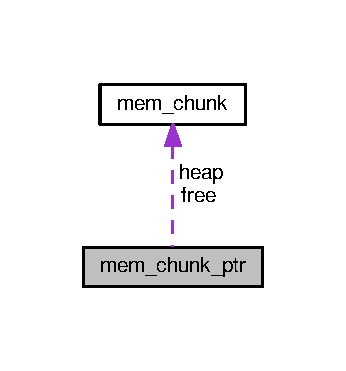
\includegraphics[width=166pt]{structmem__chunk__ptr__coll__graph}
\end{center}
\end{figure}
\subsection*{Data Fields}
\begin{DoxyCompactItemize}
\item 
\hyperlink{structmem__chunk}{mem\+\_\+chunk} $\ast$ \hyperlink{structmem__chunk__ptr_af7a1f60b420bd7ef98dde5a4cbc5bdf3}{free}
\item 
\hyperlink{structmem__chunk}{mem\+\_\+chunk} $\ast$ \hyperlink{structmem__chunk__ptr_aaddfb089e921369846e272d2d2b56e84}{heap}
\end{DoxyCompactItemize}


\subsection{Field Documentation}
\mbox{\Hypertarget{structmem__chunk__ptr_af7a1f60b420bd7ef98dde5a4cbc5bdf3}\label{structmem__chunk__ptr_af7a1f60b420bd7ef98dde5a4cbc5bdf3}} 
\index{mem\+\_\+chunk\+\_\+ptr@{mem\+\_\+chunk\+\_\+ptr}!free@{free}}
\index{free@{free}!mem\+\_\+chunk\+\_\+ptr@{mem\+\_\+chunk\+\_\+ptr}}
\subsubsection{\texorpdfstring{free}{free}}
{\footnotesize\ttfamily \hyperlink{structmem__chunk}{mem\+\_\+chunk}$\ast$ mem\+\_\+chunk\+\_\+ptr\+::free}

\mbox{\Hypertarget{structmem__chunk__ptr_aaddfb089e921369846e272d2d2b56e84}\label{structmem__chunk__ptr_aaddfb089e921369846e272d2d2b56e84}} 
\index{mem\+\_\+chunk\+\_\+ptr@{mem\+\_\+chunk\+\_\+ptr}!heap@{heap}}
\index{heap@{heap}!mem\+\_\+chunk\+\_\+ptr@{mem\+\_\+chunk\+\_\+ptr}}
\subsubsection{\texorpdfstring{heap}{heap}}
{\footnotesize\ttfamily \hyperlink{structmem__chunk}{mem\+\_\+chunk}$\ast$ mem\+\_\+chunk\+\_\+ptr\+::heap}



The documentation for this struct was generated from the following file\+:\begin{DoxyCompactItemize}
\item 
sys/include/\hyperlink{malloc_8h}{malloc.\+h}\end{DoxyCompactItemize}

\hypertarget{unionmem__header__union}{}\section{mem\+\_\+header\+\_\+union Union Reference}
\label{unionmem__header__union}\index{mem\+\_\+header\+\_\+union@{mem\+\_\+header\+\_\+union}}


{\ttfamily \#include $<$malloc.\+h$>$}



Collaboration diagram for mem\+\_\+header\+\_\+union\+:\nopagebreak
\begin{figure}[H]
\begin{center}
\leavevmode
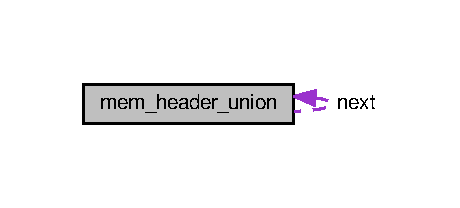
\includegraphics[width=221pt]{unionmem__header__union__coll__graph}
\end{center}
\end{figure}
\subsection*{Data Fields}
\begin{DoxyCompactItemize}
\item 
\begin{tabbing}
xx\=xx\=xx\=xx\=xx\=xx\=xx\=xx\=xx\=\kill
struct \{\\
\>union \hyperlink{unionmem__header__union}{mem\_header\_union} $\ast$ \hyperlink{unionmem__header__union_a22eb41be35488312c1e42462d5679d64}{next}\\
\>uint32\_t \hyperlink{unionmem__header__union_ab0a6578a8d52fd76a933d21273e73e08}{size}\\
\} \hyperlink{unionmem__header__union_a8e9bc77f2cf7596a7503f50ef29019f9}{s}\\

\end{tabbing}\item 
\hyperlink{malloc_8h_a1e0a98b5055eebe08414396335357f7f}{align} \hyperlink{unionmem__header__union_a5ca4f0da25cd2b76029162df7bdb537c}{align\+\_\+dummy}
\end{DoxyCompactItemize}


\subsection{Field Documentation}
\mbox{\Hypertarget{unionmem__header__union_a5ca4f0da25cd2b76029162df7bdb537c}\label{unionmem__header__union_a5ca4f0da25cd2b76029162df7bdb537c}} 
\index{mem\+\_\+header\+\_\+union@{mem\+\_\+header\+\_\+union}!align\+\_\+dummy@{align\+\_\+dummy}}
\index{align\+\_\+dummy@{align\+\_\+dummy}!mem\+\_\+header\+\_\+union@{mem\+\_\+header\+\_\+union}}
\subsubsection{\texorpdfstring{align\+\_\+dummy}{align\_dummy}}
{\footnotesize\ttfamily \hyperlink{malloc_8h_a1e0a98b5055eebe08414396335357f7f}{align} mem\+\_\+header\+\_\+union\+::align\+\_\+dummy}

\mbox{\Hypertarget{unionmem__header__union_a22eb41be35488312c1e42462d5679d64}\label{unionmem__header__union_a22eb41be35488312c1e42462d5679d64}} 
\index{mem\+\_\+header\+\_\+union@{mem\+\_\+header\+\_\+union}!next@{next}}
\index{next@{next}!mem\+\_\+header\+\_\+union@{mem\+\_\+header\+\_\+union}}
\subsubsection{\texorpdfstring{next}{next}}
{\footnotesize\ttfamily union \hyperlink{unionmem__header__union}{mem\+\_\+header\+\_\+union}$\ast$ mem\+\_\+header\+\_\+union\+::next}

\mbox{\Hypertarget{unionmem__header__union_a8e9bc77f2cf7596a7503f50ef29019f9}\label{unionmem__header__union_a8e9bc77f2cf7596a7503f50ef29019f9}} 
\index{mem\+\_\+header\+\_\+union@{mem\+\_\+header\+\_\+union}!s@{s}}
\index{s@{s}!mem\+\_\+header\+\_\+union@{mem\+\_\+header\+\_\+union}}
\subsubsection{\texorpdfstring{s}{s}}
{\footnotesize\ttfamily struct \{ ... \}   mem\+\_\+header\+\_\+union\+::s}

\mbox{\Hypertarget{unionmem__header__union_ab0a6578a8d52fd76a933d21273e73e08}\label{unionmem__header__union_ab0a6578a8d52fd76a933d21273e73e08}} 
\index{mem\+\_\+header\+\_\+union@{mem\+\_\+header\+\_\+union}!size@{size}}
\index{size@{size}!mem\+\_\+header\+\_\+union@{mem\+\_\+header\+\_\+union}}
\subsubsection{\texorpdfstring{size}{size}}
{\footnotesize\ttfamily uint32\+\_\+t mem\+\_\+header\+\_\+union\+::size}



The documentation for this union was generated from the following file\+:\begin{DoxyCompactItemize}
\item 
sys/include/\hyperlink{malloc_8h}{malloc.\+h}\end{DoxyCompactItemize}

\hypertarget{structmtx}{}\section{mtx Struct Reference}
\label{structmtx}\index{mtx@{mtx}}


Mutex data structure.  




{\ttfamily \#include $<$mutex.\+h$>$}

\subsection*{Data Fields}
\begin{DoxyCompactItemize}
\item 
int32\+\_\+t \hyperlink{structmtx_a5c9abfe5d985f974f920b19b94890f40}{lock}
\item 
uint8\+\_\+t \hyperlink{structmtx_ab13e9d09a96e18160571b960e4e7c1fb}{level} \mbox{[}M\+A\+X\+\_\+\+T\+A\+S\+KS\mbox{]}
\item 
uint8\+\_\+t \hyperlink{structmtx_a14e1d218cc3d0cd3e74ae6de1eb69212}{waiting} \mbox{[}M\+A\+X\+\_\+\+T\+A\+S\+KS -\/ 1\mbox{]}
\end{DoxyCompactItemize}


\subsection{Detailed Description}
Mutex data structure. 

\subsection{Field Documentation}
\mbox{\Hypertarget{structmtx_ab13e9d09a96e18160571b960e4e7c1fb}\label{structmtx_ab13e9d09a96e18160571b960e4e7c1fb}} 
\index{mtx@{mtx}!level@{level}}
\index{level@{level}!mtx@{mtx}}
\subsubsection{\texorpdfstring{level}{level}}
{\footnotesize\ttfamily uint8\+\_\+t mtx\+::level\mbox{[}M\+A\+X\+\_\+\+T\+A\+S\+KS\mbox{]}}

\mbox{\Hypertarget{structmtx_a5c9abfe5d985f974f920b19b94890f40}\label{structmtx_a5c9abfe5d985f974f920b19b94890f40}} 
\index{mtx@{mtx}!lock@{lock}}
\index{lock@{lock}!mtx@{mtx}}
\subsubsection{\texorpdfstring{lock}{lock}}
{\footnotesize\ttfamily int32\+\_\+t mtx\+::lock}

mutex lock, atomically modified \mbox{\Hypertarget{structmtx_a14e1d218cc3d0cd3e74ae6de1eb69212}\label{structmtx_a14e1d218cc3d0cd3e74ae6de1eb69212}} 
\index{mtx@{mtx}!waiting@{waiting}}
\index{waiting@{waiting}!mtx@{mtx}}
\subsubsection{\texorpdfstring{waiting}{waiting}}
{\footnotesize\ttfamily uint8\+\_\+t mtx\+::waiting\mbox{[}M\+A\+X\+\_\+\+T\+A\+S\+KS -\/ 1\mbox{]}}



The documentation for this struct was generated from the following file\+:\begin{DoxyCompactItemize}
\item 
sys/include/\hyperlink{mutex_8h}{mutex.\+h}\end{DoxyCompactItemize}

\hypertarget{structpcb__entry}{}\section{pcb\+\_\+entry Struct Reference}
\label{structpcb__entry}\index{pcb\+\_\+entry@{pcb\+\_\+entry}}


{\ttfamily \#include $<$kernel.\+h$>$}

\subsection*{Data Fields}
\begin{DoxyCompactItemize}
\item 
int32\+\_\+t($\ast$ \hyperlink{structpcb__entry_afed67ff0db4482a197f9f98085c29724}{sched\+\_\+rt} )()
\item 
int32\+\_\+t($\ast$ \hyperlink{structpcb__entry_ab1848ecd2c321b6a19e80f0148beb053}{sched\+\_\+be} )()
\item 
uint32\+\_\+t \hyperlink{structpcb__entry_ac5899befd89fa0e8b2aeceed85e01415}{coop\+\_\+cswitch}
\item 
uint32\+\_\+t \hyperlink{structpcb__entry_af49c7195c79f5de2d70825e2252c8d77}{preempt\+\_\+cswitch}
\item 
uint32\+\_\+t \hyperlink{structpcb__entry_ae5474e1d477335caf5515d8a940d1f77}{interrupts}
\item 
uint32\+\_\+t \hyperlink{structpcb__entry_a998d1bf7b5ac3d6b0b9c4c6c7a0ebec6}{tick\+\_\+time}
\end{DoxyCompactItemize}


\subsection{Field Documentation}
\mbox{\Hypertarget{structpcb__entry_ac5899befd89fa0e8b2aeceed85e01415}\label{structpcb__entry_ac5899befd89fa0e8b2aeceed85e01415}} 
\index{pcb\+\_\+entry@{pcb\+\_\+entry}!coop\+\_\+cswitch@{coop\+\_\+cswitch}}
\index{coop\+\_\+cswitch@{coop\+\_\+cswitch}!pcb\+\_\+entry@{pcb\+\_\+entry}}
\subsubsection{\texorpdfstring{coop\+\_\+cswitch}{coop\_cswitch}}
{\footnotesize\ttfamily uint32\+\_\+t pcb\+\_\+entry\+::coop\+\_\+cswitch}

cooperative context switches \mbox{\Hypertarget{structpcb__entry_ae5474e1d477335caf5515d8a940d1f77}\label{structpcb__entry_ae5474e1d477335caf5515d8a940d1f77}} 
\index{pcb\+\_\+entry@{pcb\+\_\+entry}!interrupts@{interrupts}}
\index{interrupts@{interrupts}!pcb\+\_\+entry@{pcb\+\_\+entry}}
\subsubsection{\texorpdfstring{interrupts}{interrupts}}
{\footnotesize\ttfamily uint32\+\_\+t pcb\+\_\+entry\+::interrupts}

number of non-\/masked interrupts \mbox{\Hypertarget{structpcb__entry_af49c7195c79f5de2d70825e2252c8d77}\label{structpcb__entry_af49c7195c79f5de2d70825e2252c8d77}} 
\index{pcb\+\_\+entry@{pcb\+\_\+entry}!preempt\+\_\+cswitch@{preempt\+\_\+cswitch}}
\index{preempt\+\_\+cswitch@{preempt\+\_\+cswitch}!pcb\+\_\+entry@{pcb\+\_\+entry}}
\subsubsection{\texorpdfstring{preempt\+\_\+cswitch}{preempt\_cswitch}}
{\footnotesize\ttfamily uint32\+\_\+t pcb\+\_\+entry\+::preempt\+\_\+cswitch}

preeptive context switches \mbox{\Hypertarget{structpcb__entry_ab1848ecd2c321b6a19e80f0148beb053}\label{structpcb__entry_ab1848ecd2c321b6a19e80f0148beb053}} 
\index{pcb\+\_\+entry@{pcb\+\_\+entry}!sched\+\_\+be@{sched\+\_\+be}}
\index{sched\+\_\+be@{sched\+\_\+be}!pcb\+\_\+entry@{pcb\+\_\+entry}}
\subsubsection{\texorpdfstring{sched\+\_\+be}{sched\_be}}
{\footnotesize\ttfamily int32\+\_\+t($\ast$ pcb\+\_\+entry\+::sched\+\_\+be) ()}

pointer to the best effort scheduler \mbox{\Hypertarget{structpcb__entry_afed67ff0db4482a197f9f98085c29724}\label{structpcb__entry_afed67ff0db4482a197f9f98085c29724}} 
\index{pcb\+\_\+entry@{pcb\+\_\+entry}!sched\+\_\+rt@{sched\+\_\+rt}}
\index{sched\+\_\+rt@{sched\+\_\+rt}!pcb\+\_\+entry@{pcb\+\_\+entry}}
\subsubsection{\texorpdfstring{sched\+\_\+rt}{sched\_rt}}
{\footnotesize\ttfamily int32\+\_\+t($\ast$ pcb\+\_\+entry\+::sched\+\_\+rt) ()}

pointer to the realtime scheduler \mbox{\Hypertarget{structpcb__entry_a998d1bf7b5ac3d6b0b9c4c6c7a0ebec6}\label{structpcb__entry_a998d1bf7b5ac3d6b0b9c4c6c7a0ebec6}} 
\index{pcb\+\_\+entry@{pcb\+\_\+entry}!tick\+\_\+time@{tick\+\_\+time}}
\index{tick\+\_\+time@{tick\+\_\+time}!pcb\+\_\+entry@{pcb\+\_\+entry}}
\subsubsection{\texorpdfstring{tick\+\_\+time}{tick\_time}}
{\footnotesize\ttfamily uint32\+\_\+t pcb\+\_\+entry\+::tick\+\_\+time}

tick time in microsseconds 

The documentation for this struct was generated from the following file\+:\begin{DoxyCompactItemize}
\item 
sys/include/\hyperlink{kernel_8h}{kernel.\+h}\end{DoxyCompactItemize}

\hypertarget{structqueue}{}\section{queue Struct Reference}
\label{structqueue}\index{queue@{queue}}


Queue data structure.  




{\ttfamily \#include $<$queue.\+h$>$}

\subsection*{Data Fields}
\begin{DoxyCompactItemize}
\item 
int32\+\_\+t \hyperlink{structqueue_af80cfabc36286195365b6d666d518504}{size}
\item 
int32\+\_\+t \hyperlink{structqueue_a187a42d061b48da53e894181758d558d}{elem}
\item 
int32\+\_\+t \hyperlink{structqueue_aec96f7889213946d685f28a0d6504428}{head}
\item 
int32\+\_\+t \hyperlink{structqueue_ada0fe9a078df1d07623c761f2e8376ad}{tail}
\item 
void $\ast$$\ast$ \hyperlink{structqueue_a794929032d575599c02f795cea4b3118}{data}
\end{DoxyCompactItemize}


\subsection{Detailed Description}
Queue data structure. 

\subsection{Field Documentation}
\mbox{\Hypertarget{structqueue_a794929032d575599c02f795cea4b3118}\label{structqueue_a794929032d575599c02f795cea4b3118}} 
\index{queue@{queue}!data@{data}}
\index{data@{data}!queue@{queue}}
\subsubsection{\texorpdfstring{data}{data}}
{\footnotesize\ttfamily void$\ast$$\ast$ queue\+::data}

pointer to an array of pointers to node data \mbox{\Hypertarget{structqueue_a187a42d061b48da53e894181758d558d}\label{structqueue_a187a42d061b48da53e894181758d558d}} 
\index{queue@{queue}!elem@{elem}}
\index{elem@{elem}!queue@{queue}}
\subsubsection{\texorpdfstring{elem}{elem}}
{\footnotesize\ttfamily int32\+\_\+t queue\+::elem}

number of elements queued \mbox{\Hypertarget{structqueue_aec96f7889213946d685f28a0d6504428}\label{structqueue_aec96f7889213946d685f28a0d6504428}} 
\index{queue@{queue}!head@{head}}
\index{head@{head}!queue@{queue}}
\subsubsection{\texorpdfstring{head}{head}}
{\footnotesize\ttfamily int32\+\_\+t queue\+::head}

first element of the queue \mbox{\Hypertarget{structqueue_af80cfabc36286195365b6d666d518504}\label{structqueue_af80cfabc36286195365b6d666d518504}} 
\index{queue@{queue}!size@{size}}
\index{size@{size}!queue@{queue}}
\subsubsection{\texorpdfstring{size}{size}}
{\footnotesize\ttfamily int32\+\_\+t queue\+::size}

queue size (maximum number of elements) \mbox{\Hypertarget{structqueue_ada0fe9a078df1d07623c761f2e8376ad}\label{structqueue_ada0fe9a078df1d07623c761f2e8376ad}} 
\index{queue@{queue}!tail@{tail}}
\index{tail@{tail}!queue@{queue}}
\subsubsection{\texorpdfstring{tail}{tail}}
{\footnotesize\ttfamily int32\+\_\+t queue\+::tail}

last element of the queue 

The documentation for this struct was generated from the following file\+:\begin{DoxyCompactItemize}
\item 
sys/include/\hyperlink{queue_8h}{queue.\+h}\end{DoxyCompactItemize}

\hypertarget{structsem}{}\section{sem Struct Reference}
\label{structsem}\index{sem@{sem}}


Semaphore data structure.  




{\ttfamily \#include $<$semaphore.\+h$>$}



Collaboration diagram for sem\+:\nopagebreak
\begin{figure}[H]
\begin{center}
\leavevmode
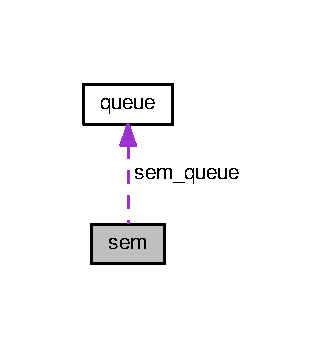
\includegraphics[width=156pt]{structsem__coll__graph}
\end{center}
\end{figure}
\subsection*{Data Fields}
\begin{DoxyCompactItemize}
\item 
struct \hyperlink{structqueue}{queue} $\ast$ \hyperlink{structsem_a723ac960b2566b855b905fa4aa324f9b}{sem\+\_\+queue}
\item 
int32\+\_\+t \hyperlink{structsem_a798dc7e825b1e632b2db49b473b17636}{count}
\end{DoxyCompactItemize}


\subsection{Detailed Description}
Semaphore data structure. 

\subsection{Field Documentation}
\mbox{\Hypertarget{structsem_a798dc7e825b1e632b2db49b473b17636}\label{structsem_a798dc7e825b1e632b2db49b473b17636}} 
\index{sem@{sem}!count@{count}}
\index{count@{count}!sem@{sem}}
\subsubsection{\texorpdfstring{count}{count}}
{\footnotesize\ttfamily int32\+\_\+t sem\+::count}

semaphore counter \mbox{\Hypertarget{structsem_a723ac960b2566b855b905fa4aa324f9b}\label{structsem_a723ac960b2566b855b905fa4aa324f9b}} 
\index{sem@{sem}!sem\+\_\+queue@{sem\+\_\+queue}}
\index{sem\+\_\+queue@{sem\+\_\+queue}!sem@{sem}}
\subsubsection{\texorpdfstring{sem\+\_\+queue}{sem\_queue}}
{\footnotesize\ttfamily struct \hyperlink{structqueue}{queue}$\ast$ sem\+::sem\+\_\+queue}

queue for tasks waiting on the semaphore 

The documentation for this struct was generated from the following file\+:\begin{DoxyCompactItemize}
\item 
sys/include/\hyperlink{semaphore_8h}{semaphore.\+h}\end{DoxyCompactItemize}

\hypertarget{structtcb__entry}{}\section{tcb\+\_\+entry Struct Reference}
\label{structtcb__entry}\index{tcb\+\_\+entry@{tcb\+\_\+entry}}


Task control block (T\+CB) and processor control block (P\+CB) entry data structures.  




{\ttfamily \#include $<$kernel.\+h$>$}

\subsection*{Data Fields}
\begin{DoxyCompactItemize}
\item 
uint16\+\_\+t \hyperlink{structtcb__entry_ac06c8d6513b9d3031956b0efc2ab4871}{id}
\item 
int8\+\_\+t \hyperlink{structtcb__entry_ad7bfcb0f4b58b797af44f3a078abebff}{name} \mbox{[}20\mbox{]}
\item 
uint8\+\_\+t \hyperlink{structtcb__entry_a67f430ab50cb8ff9133e133fc240f3d7}{state}
\item 
uint8\+\_\+t \hyperlink{structtcb__entry_a5a925d67b6f5391815abcbd2c251c77d}{priority}
\item 
uint8\+\_\+t \hyperlink{structtcb__entry_a63888ca7a7a923f912bf3a404d1261ca}{priority\+\_\+rem}
\item 
uint8\+\_\+t \hyperlink{structtcb__entry_ab76fc52c033f2b9cd0adc9474fcde5ef}{critical}
\item 
uint32\+\_\+t \hyperlink{structtcb__entry_ab29fad6168f140493ddc8f860fadc3bc}{delay}
\item 
uint32\+\_\+t \hyperlink{structtcb__entry_a51802bc7ba3ee4cfcbcbfb404e606643}{rtjobs}
\item 
uint32\+\_\+t \hyperlink{structtcb__entry_a27631962295edabd283477b471f2d7ae}{bgjobs}
\item 
uint32\+\_\+t \hyperlink{structtcb__entry_a4594d17577feba0bd0825c8ef5e693db}{deadline\+\_\+misses}
\item 
uint16\+\_\+t \hyperlink{structtcb__entry_a85e14b4c040e0535b45b52a7ee7c9a94}{period}
\item 
uint16\+\_\+t \hyperlink{structtcb__entry_a2a3c8e5e81c910ccd845a8d1f58d550a}{capacity}
\item 
uint16\+\_\+t \hyperlink{structtcb__entry_a14ef4f38d7589e42ac7847b2bcc3443f}{deadline}
\item 
uint16\+\_\+t \hyperlink{structtcb__entry_a559dce8ac2982d3c8f46808ddc52bbb9}{capacity\+\_\+rem}
\item 
uint16\+\_\+t \hyperlink{structtcb__entry_af2ba0dde6c7ae71b6341714bf096cc80}{deadline\+\_\+rem}
\item 
context \hyperlink{structtcb__entry_a589e6c94b17a97df5d22edf504acfd42}{task\+\_\+context}
\item 
void($\ast$ \hyperlink{structtcb__entry_ae22d4a7aaefabed03dbfcb18633063e2}{ptask} )(void)
\item 
size\+\_\+t $\ast$ \hyperlink{structtcb__entry_a48bcced7fc892ae8db7138786e38a898}{pstack}
\item 
uint32\+\_\+t \hyperlink{structtcb__entry_a2174ff4c5cf178e9dc3d652c472b23dd}{stack\+\_\+size}
\item 
void $\ast$ \hyperlink{structtcb__entry_accd675f017bb0ec5ae63b4d729bd73aa}{other\+\_\+data}
\end{DoxyCompactItemize}


\subsection{Detailed Description}
Task control block (T\+CB) and processor control block (P\+CB) entry data structures. 

\subsection{Field Documentation}
\mbox{\Hypertarget{structtcb__entry_a27631962295edabd283477b471f2d7ae}\label{structtcb__entry_a27631962295edabd283477b471f2d7ae}} 
\index{tcb\+\_\+entry@{tcb\+\_\+entry}!bgjobs@{bgjobs}}
\index{bgjobs@{bgjobs}!tcb\+\_\+entry@{tcb\+\_\+entry}}
\subsubsection{\texorpdfstring{bgjobs}{bgjobs}}
{\footnotesize\ttfamily uint32\+\_\+t tcb\+\_\+entry\+::bgjobs}

total BE task jobs executed \mbox{\Hypertarget{structtcb__entry_a2a3c8e5e81c910ccd845a8d1f58d550a}\label{structtcb__entry_a2a3c8e5e81c910ccd845a8d1f58d550a}} 
\index{tcb\+\_\+entry@{tcb\+\_\+entry}!capacity@{capacity}}
\index{capacity@{capacity}!tcb\+\_\+entry@{tcb\+\_\+entry}}
\subsubsection{\texorpdfstring{capacity}{capacity}}
{\footnotesize\ttfamily uint16\+\_\+t tcb\+\_\+entry\+::capacity}

task capacity \mbox{\Hypertarget{structtcb__entry_a559dce8ac2982d3c8f46808ddc52bbb9}\label{structtcb__entry_a559dce8ac2982d3c8f46808ddc52bbb9}} 
\index{tcb\+\_\+entry@{tcb\+\_\+entry}!capacity\+\_\+rem@{capacity\+\_\+rem}}
\index{capacity\+\_\+rem@{capacity\+\_\+rem}!tcb\+\_\+entry@{tcb\+\_\+entry}}
\subsubsection{\texorpdfstring{capacity\+\_\+rem}{capacity\_rem}}
{\footnotesize\ttfamily uint16\+\_\+t tcb\+\_\+entry\+::capacity\+\_\+rem}

remaining capacity on period \mbox{\Hypertarget{structtcb__entry_ab76fc52c033f2b9cd0adc9474fcde5ef}\label{structtcb__entry_ab76fc52c033f2b9cd0adc9474fcde5ef}} 
\index{tcb\+\_\+entry@{tcb\+\_\+entry}!critical@{critical}}
\index{critical@{critical}!tcb\+\_\+entry@{tcb\+\_\+entry}}
\subsubsection{\texorpdfstring{critical}{critical}}
{\footnotesize\ttfamily uint8\+\_\+t tcb\+\_\+entry\+::critical}

critical event, interrupt request \mbox{\Hypertarget{structtcb__entry_a14ef4f38d7589e42ac7847b2bcc3443f}\label{structtcb__entry_a14ef4f38d7589e42ac7847b2bcc3443f}} 
\index{tcb\+\_\+entry@{tcb\+\_\+entry}!deadline@{deadline}}
\index{deadline@{deadline}!tcb\+\_\+entry@{tcb\+\_\+entry}}
\subsubsection{\texorpdfstring{deadline}{deadline}}
{\footnotesize\ttfamily uint16\+\_\+t tcb\+\_\+entry\+::deadline}

task deadline \mbox{\Hypertarget{structtcb__entry_a4594d17577feba0bd0825c8ef5e693db}\label{structtcb__entry_a4594d17577feba0bd0825c8ef5e693db}} 
\index{tcb\+\_\+entry@{tcb\+\_\+entry}!deadline\+\_\+misses@{deadline\+\_\+misses}}
\index{deadline\+\_\+misses@{deadline\+\_\+misses}!tcb\+\_\+entry@{tcb\+\_\+entry}}
\subsubsection{\texorpdfstring{deadline\+\_\+misses}{deadline\_misses}}
{\footnotesize\ttfamily uint32\+\_\+t tcb\+\_\+entry\+::deadline\+\_\+misses}

task realtime deadline misses \mbox{\Hypertarget{structtcb__entry_af2ba0dde6c7ae71b6341714bf096cc80}\label{structtcb__entry_af2ba0dde6c7ae71b6341714bf096cc80}} 
\index{tcb\+\_\+entry@{tcb\+\_\+entry}!deadline\+\_\+rem@{deadline\+\_\+rem}}
\index{deadline\+\_\+rem@{deadline\+\_\+rem}!tcb\+\_\+entry@{tcb\+\_\+entry}}
\subsubsection{\texorpdfstring{deadline\+\_\+rem}{deadline\_rem}}
{\footnotesize\ttfamily uint16\+\_\+t tcb\+\_\+entry\+::deadline\+\_\+rem}

remaining time slices on period \mbox{\Hypertarget{structtcb__entry_ab29fad6168f140493ddc8f860fadc3bc}\label{structtcb__entry_ab29fad6168f140493ddc8f860fadc3bc}} 
\index{tcb\+\_\+entry@{tcb\+\_\+entry}!delay@{delay}}
\index{delay@{delay}!tcb\+\_\+entry@{tcb\+\_\+entry}}
\subsubsection{\texorpdfstring{delay}{delay}}
{\footnotesize\ttfamily uint32\+\_\+t tcb\+\_\+entry\+::delay}

delay to enter in the run/\+RT queue \mbox{\Hypertarget{structtcb__entry_ac06c8d6513b9d3031956b0efc2ab4871}\label{structtcb__entry_ac06c8d6513b9d3031956b0efc2ab4871}} 
\index{tcb\+\_\+entry@{tcb\+\_\+entry}!id@{id}}
\index{id@{id}!tcb\+\_\+entry@{tcb\+\_\+entry}}
\subsubsection{\texorpdfstring{id}{id}}
{\footnotesize\ttfamily uint16\+\_\+t tcb\+\_\+entry\+::id}

task id \mbox{\Hypertarget{structtcb__entry_ad7bfcb0f4b58b797af44f3a078abebff}\label{structtcb__entry_ad7bfcb0f4b58b797af44f3a078abebff}} 
\index{tcb\+\_\+entry@{tcb\+\_\+entry}!name@{name}}
\index{name@{name}!tcb\+\_\+entry@{tcb\+\_\+entry}}
\subsubsection{\texorpdfstring{name}{name}}
{\footnotesize\ttfamily int8\+\_\+t tcb\+\_\+entry\+::name\mbox{[}20\mbox{]}}

task description (or name) \mbox{\Hypertarget{structtcb__entry_accd675f017bb0ec5ae63b4d729bd73aa}\label{structtcb__entry_accd675f017bb0ec5ae63b4d729bd73aa}} 
\index{tcb\+\_\+entry@{tcb\+\_\+entry}!other\+\_\+data@{other\+\_\+data}}
\index{other\+\_\+data@{other\+\_\+data}!tcb\+\_\+entry@{tcb\+\_\+entry}}
\subsubsection{\texorpdfstring{other\+\_\+data}{other\_data}}
{\footnotesize\ttfamily void$\ast$ tcb\+\_\+entry\+::other\+\_\+data}

pointer to other data related to this task \mbox{\Hypertarget{structtcb__entry_a85e14b4c040e0535b45b52a7ee7c9a94}\label{structtcb__entry_a85e14b4c040e0535b45b52a7ee7c9a94}} 
\index{tcb\+\_\+entry@{tcb\+\_\+entry}!period@{period}}
\index{period@{period}!tcb\+\_\+entry@{tcb\+\_\+entry}}
\subsubsection{\texorpdfstring{period}{period}}
{\footnotesize\ttfamily uint16\+\_\+t tcb\+\_\+entry\+::period}

task period \mbox{\Hypertarget{structtcb__entry_a5a925d67b6f5391815abcbd2c251c77d}\label{structtcb__entry_a5a925d67b6f5391815abcbd2c251c77d}} 
\index{tcb\+\_\+entry@{tcb\+\_\+entry}!priority@{priority}}
\index{priority@{priority}!tcb\+\_\+entry@{tcb\+\_\+entry}}
\subsubsection{\texorpdfstring{priority}{priority}}
{\footnotesize\ttfamily uint8\+\_\+t tcb\+\_\+entry\+::priority}

\mbox{[}1 .. 29\mbox{]} -\/ critical, \mbox{[}30 .. 99\mbox{]} -\/ system, \mbox{[}100 .. 255\mbox{]} -\/ application \mbox{\Hypertarget{structtcb__entry_a63888ca7a7a923f912bf3a404d1261ca}\label{structtcb__entry_a63888ca7a7a923f912bf3a404d1261ca}} 
\index{tcb\+\_\+entry@{tcb\+\_\+entry}!priority\+\_\+rem@{priority\+\_\+rem}}
\index{priority\+\_\+rem@{priority\+\_\+rem}!tcb\+\_\+entry@{tcb\+\_\+entry}}
\subsubsection{\texorpdfstring{priority\+\_\+rem}{priority\_rem}}
{\footnotesize\ttfamily uint8\+\_\+t tcb\+\_\+entry\+::priority\+\_\+rem}

remaining priority \mbox{\Hypertarget{structtcb__entry_a48bcced7fc892ae8db7138786e38a898}\label{structtcb__entry_a48bcced7fc892ae8db7138786e38a898}} 
\index{tcb\+\_\+entry@{tcb\+\_\+entry}!pstack@{pstack}}
\index{pstack@{pstack}!tcb\+\_\+entry@{tcb\+\_\+entry}}
\subsubsection{\texorpdfstring{pstack}{pstack}}
{\footnotesize\ttfamily size\+\_\+t$\ast$ tcb\+\_\+entry\+::pstack}

task stack area (bottom) \mbox{\Hypertarget{structtcb__entry_ae22d4a7aaefabed03dbfcb18633063e2}\label{structtcb__entry_ae22d4a7aaefabed03dbfcb18633063e2}} 
\index{tcb\+\_\+entry@{tcb\+\_\+entry}!ptask@{ptask}}
\index{ptask@{ptask}!tcb\+\_\+entry@{tcb\+\_\+entry}}
\subsubsection{\texorpdfstring{ptask}{ptask}}
{\footnotesize\ttfamily void($\ast$ tcb\+\_\+entry\+::ptask) (void)}

task entry point, pointer to function \mbox{\Hypertarget{structtcb__entry_a51802bc7ba3ee4cfcbcbfb404e606643}\label{structtcb__entry_a51802bc7ba3ee4cfcbcbfb404e606643}} 
\index{tcb\+\_\+entry@{tcb\+\_\+entry}!rtjobs@{rtjobs}}
\index{rtjobs@{rtjobs}!tcb\+\_\+entry@{tcb\+\_\+entry}}
\subsubsection{\texorpdfstring{rtjobs}{rtjobs}}
{\footnotesize\ttfamily uint32\+\_\+t tcb\+\_\+entry\+::rtjobs}

total RT task jobs executed \mbox{\Hypertarget{structtcb__entry_a2174ff4c5cf178e9dc3d652c472b23dd}\label{structtcb__entry_a2174ff4c5cf178e9dc3d652c472b23dd}} 
\index{tcb\+\_\+entry@{tcb\+\_\+entry}!stack\+\_\+size@{stack\+\_\+size}}
\index{stack\+\_\+size@{stack\+\_\+size}!tcb\+\_\+entry@{tcb\+\_\+entry}}
\subsubsection{\texorpdfstring{stack\+\_\+size}{stack\_size}}
{\footnotesize\ttfamily uint32\+\_\+t tcb\+\_\+entry\+::stack\+\_\+size}

task stack size \mbox{\Hypertarget{structtcb__entry_a67f430ab50cb8ff9133e133fc240f3d7}\label{structtcb__entry_a67f430ab50cb8ff9133e133fc240f3d7}} 
\index{tcb\+\_\+entry@{tcb\+\_\+entry}!state@{state}}
\index{state@{state}!tcb\+\_\+entry@{tcb\+\_\+entry}}
\subsubsection{\texorpdfstring{state}{state}}
{\footnotesize\ttfamily uint8\+\_\+t tcb\+\_\+entry\+::state}

0 -\/ idle, 1 -\/ ready, 2 -\/ running, 3 -\/ blocked, 4 -\/ delayed, 5 -\/ waiting \mbox{\Hypertarget{structtcb__entry_a589e6c94b17a97df5d22edf504acfd42}\label{structtcb__entry_a589e6c94b17a97df5d22edf504acfd42}} 
\index{tcb\+\_\+entry@{tcb\+\_\+entry}!task\+\_\+context@{task\+\_\+context}}
\index{task\+\_\+context@{task\+\_\+context}!tcb\+\_\+entry@{tcb\+\_\+entry}}
\subsubsection{\texorpdfstring{task\+\_\+context}{task\_context}}
{\footnotesize\ttfamily context tcb\+\_\+entry\+::task\+\_\+context}

task context 

The documentation for this struct was generated from the following file\+:\begin{DoxyCompactItemize}
\item 
sys/include/\hyperlink{kernel_8h}{kernel.\+h}\end{DoxyCompactItemize}

\hypertarget{structuudp}{}\section{uudp Struct Reference}
\label{structuudp}\index{uudp@{uudp}}


{\ttfamily \#include $<$uudp.\+h$>$}



Collaboration diagram for uudp\+:\nopagebreak
\begin{figure}[H]
\begin{center}
\leavevmode
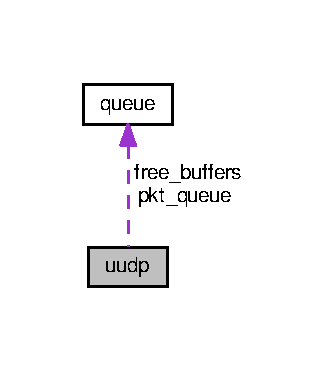
\includegraphics[width=157pt]{structuudp__coll__graph}
\end{center}
\end{figure}
\subsection*{Data Fields}
\begin{DoxyCompactItemize}
\item 
uint16\+\_\+t \hyperlink{structuudp_a00e34c9d365186d751ac02d8fd8fb130}{listen\+\_\+port}
\item 
struct \hyperlink{structqueue}{queue} $\ast$ \hyperlink{structuudp_a82b920ae77d6f50adebe104fde7bd372}{free\+\_\+buffers}
\item 
struct \hyperlink{structqueue}{queue} $\ast$ \hyperlink{structuudp_a173d6e92d93ed6c5a8e6bae66a66c132}{pkt\+\_\+queue}
\end{DoxyCompactItemize}


\subsection{Field Documentation}
\mbox{\Hypertarget{structuudp_a82b920ae77d6f50adebe104fde7bd372}\label{structuudp_a82b920ae77d6f50adebe104fde7bd372}} 
\index{uudp@{uudp}!free\+\_\+buffers@{free\+\_\+buffers}}
\index{free\+\_\+buffers@{free\+\_\+buffers}!uudp@{uudp}}
\subsubsection{\texorpdfstring{free\+\_\+buffers}{free\_buffers}}
{\footnotesize\ttfamily struct \hyperlink{structqueue}{queue}$\ast$ uudp\+::free\+\_\+buffers}

\mbox{\Hypertarget{structuudp_a00e34c9d365186d751ac02d8fd8fb130}\label{structuudp_a00e34c9d365186d751ac02d8fd8fb130}} 
\index{uudp@{uudp}!listen\+\_\+port@{listen\+\_\+port}}
\index{listen\+\_\+port@{listen\+\_\+port}!uudp@{uudp}}
\subsubsection{\texorpdfstring{listen\+\_\+port}{listen\_port}}
{\footnotesize\ttfamily uint16\+\_\+t uudp\+::listen\+\_\+port}

\mbox{\Hypertarget{structuudp_a173d6e92d93ed6c5a8e6bae66a66c132}\label{structuudp_a173d6e92d93ed6c5a8e6bae66a66c132}} 
\index{uudp@{uudp}!pkt\+\_\+queue@{pkt\+\_\+queue}}
\index{pkt\+\_\+queue@{pkt\+\_\+queue}!uudp@{uudp}}
\subsubsection{\texorpdfstring{pkt\+\_\+queue}{pkt\_queue}}
{\footnotesize\ttfamily struct \hyperlink{structqueue}{queue}$\ast$ uudp\+::pkt\+\_\+queue}



The documentation for this struct was generated from the following file\+:\begin{DoxyCompactItemize}
\item 
net/include/\hyperlink{uudp_8h}{uudp.\+h}\end{DoxyCompactItemize}

\chapter{File Documentation}
\hypertarget{ni__generic_8h}{}\section{drivers/noc/include/ni\+\_\+generic.h File Reference}
\label{ni__generic_8h}\index{drivers/noc/include/ni\+\_\+generic.\+h@{drivers/noc/include/ni\+\_\+generic.\+h}}
\subsection*{Functions}
\begin{DoxyCompactItemize}
\item 
int32\+\_\+t \hyperlink{ni__generic_8h_ac935a14a6eed5d7cacb21ecc72ec2fa5}{ni\+\_\+ready} (void)
\item 
int32\+\_\+t \hyperlink{ni__generic_8h_a440c71c3a4d4c4f5704de080f85f1428}{ni\+\_\+flush} (uint16\+\_\+t pkt\+\_\+size)
\item 
int32\+\_\+t \hyperlink{ni__generic_8h_a7185a5c02c3e5dd69df562a2cc3033b1}{ni\+\_\+read\+\_\+packet} (uint16\+\_\+t $\ast$buf, uint16\+\_\+t pkt\+\_\+size)
\item 
int32\+\_\+t \hyperlink{ni__generic_8h_a29d4f0701c32bc2cb4812bfde7e26f01}{ni\+\_\+write\+\_\+packet} (uint16\+\_\+t $\ast$buf, uint16\+\_\+t pkt\+\_\+size)
\end{DoxyCompactItemize}


\subsection{Function Documentation}
\mbox{\Hypertarget{ni__generic_8h_a440c71c3a4d4c4f5704de080f85f1428}\label{ni__generic_8h_a440c71c3a4d4c4f5704de080f85f1428}} 
\index{ni\+\_\+generic.\+h@{ni\+\_\+generic.\+h}!ni\+\_\+flush@{ni\+\_\+flush}}
\index{ni\+\_\+flush@{ni\+\_\+flush}!ni\+\_\+generic.\+h@{ni\+\_\+generic.\+h}}
\subsubsection{\texorpdfstring{ni\+\_\+flush()}{ni\_flush()}}
{\footnotesize\ttfamily int32\+\_\+t ni\+\_\+flush (\begin{DoxyParamCaption}\item[{uint16\+\_\+t}]{pkt\+\_\+size }\end{DoxyParamCaption})}

\mbox{\Hypertarget{ni__generic_8h_a7185a5c02c3e5dd69df562a2cc3033b1}\label{ni__generic_8h_a7185a5c02c3e5dd69df562a2cc3033b1}} 
\index{ni\+\_\+generic.\+h@{ni\+\_\+generic.\+h}!ni\+\_\+read\+\_\+packet@{ni\+\_\+read\+\_\+packet}}
\index{ni\+\_\+read\+\_\+packet@{ni\+\_\+read\+\_\+packet}!ni\+\_\+generic.\+h@{ni\+\_\+generic.\+h}}
\subsubsection{\texorpdfstring{ni\+\_\+read\+\_\+packet()}{ni\_read\_packet()}}
{\footnotesize\ttfamily int32\+\_\+t ni\+\_\+read\+\_\+packet (\begin{DoxyParamCaption}\item[{uint16\+\_\+t $\ast$}]{buf,  }\item[{uint16\+\_\+t}]{pkt\+\_\+size }\end{DoxyParamCaption})}

\mbox{\Hypertarget{ni__generic_8h_ac935a14a6eed5d7cacb21ecc72ec2fa5}\label{ni__generic_8h_ac935a14a6eed5d7cacb21ecc72ec2fa5}} 
\index{ni\+\_\+generic.\+h@{ni\+\_\+generic.\+h}!ni\+\_\+ready@{ni\+\_\+ready}}
\index{ni\+\_\+ready@{ni\+\_\+ready}!ni\+\_\+generic.\+h@{ni\+\_\+generic.\+h}}
\subsubsection{\texorpdfstring{ni\+\_\+ready()}{ni\_ready()}}
{\footnotesize\ttfamily int32\+\_\+t ni\+\_\+ready (\begin{DoxyParamCaption}\item[{void}]{ }\end{DoxyParamCaption})}

\mbox{\Hypertarget{ni__generic_8h_a29d4f0701c32bc2cb4812bfde7e26f01}\label{ni__generic_8h_a29d4f0701c32bc2cb4812bfde7e26f01}} 
\index{ni\+\_\+generic.\+h@{ni\+\_\+generic.\+h}!ni\+\_\+write\+\_\+packet@{ni\+\_\+write\+\_\+packet}}
\index{ni\+\_\+write\+\_\+packet@{ni\+\_\+write\+\_\+packet}!ni\+\_\+generic.\+h@{ni\+\_\+generic.\+h}}
\subsubsection{\texorpdfstring{ni\+\_\+write\+\_\+packet()}{ni\_write\_packet()}}
{\footnotesize\ttfamily int32\+\_\+t ni\+\_\+write\+\_\+packet (\begin{DoxyParamCaption}\item[{uint16\+\_\+t $\ast$}]{buf,  }\item[{uint16\+\_\+t}]{pkt\+\_\+size }\end{DoxyParamCaption})}


\hypertarget{noc_8h}{}\section{drivers/noc/include/noc.h File Reference}
\label{noc_8h}\index{drivers/noc/include/noc.\+h@{drivers/noc/include/noc.\+h}}
\subsection*{Functions}
\begin{DoxyCompactItemize}
\item 
void \hyperlink{noc_8h_acb44cf0de3a986b823c53d881bff9568}{ni\+\_\+init} (void)
\begin{DoxyCompactList}\small\item\em NoC driver\+: initializes the network interface. \end{DoxyCompactList}\item 
void \hyperlink{noc_8h_a7ca8f6357767be7d8d8f31a1f68902a1}{ni\+\_\+isr} (void $\ast$arg)
\begin{DoxyCompactList}\small\item\em NoC driver\+: network interface interrupt service routine. \end{DoxyCompactList}\item 
uint16\+\_\+t \hyperlink{noc_8h_a73af25121fa7d699224d30913bb3cfa9}{hf\+\_\+cpuid} (void)
\begin{DoxyCompactList}\small\item\em Returns the current cpu id number. \end{DoxyCompactList}\item 
uint16\+\_\+t \hyperlink{noc_8h_ac100d0cfa54da4cf1c8ffda0947a7509}{hf\+\_\+ncores} (void)
\begin{DoxyCompactList}\small\item\em Returns the number of processors in the system. \end{DoxyCompactList}\item 
int32\+\_\+t \hyperlink{noc_8h_a7cc950118783aff78ef381c30f411f31}{hf\+\_\+comm\+\_\+create} (uint16\+\_\+t id, uint16\+\_\+t port, uint16\+\_\+t packets)
\begin{DoxyCompactList}\small\item\em Creates a communication queue for a task, using a port number as an alias. \end{DoxyCompactList}\item 
int32\+\_\+t \hyperlink{noc_8h_a2ca5bce1d7d281b5ca1ee007b170143b}{hf\+\_\+comm\+\_\+destroy} (uint16\+\_\+t id)
\begin{DoxyCompactList}\small\item\em Destroys a communication queue, returning packets buffered on a task message queue to the shared pool of packets. \end{DoxyCompactList}\item 
int32\+\_\+t \hyperlink{noc_8h_a29ba40363b28033d801aca0933cc64af}{hf\+\_\+recvprobe} (void)
\begin{DoxyCompactList}\small\item\em Probes for a message from a task. \end{DoxyCompactList}\item 
int32\+\_\+t \hyperlink{noc_8h_a27bdcde2185022f68eece2e0ed1c20ec}{hf\+\_\+recv} (uint16\+\_\+t $\ast$source\+\_\+cpu, uint16\+\_\+t $\ast$source\+\_\+port, int8\+\_\+t $\ast$buf, uint16\+\_\+t $\ast$size, uint16\+\_\+t channel)
\begin{DoxyCompactList}\small\item\em Receives a message from a task (blocking receive). \end{DoxyCompactList}\item 
int32\+\_\+t \hyperlink{noc_8h_ae7c110f06bc1e123f03b2d52d8b6d70f}{hf\+\_\+send} (uint16\+\_\+t target\+\_\+cpu, uint16\+\_\+t target\+\_\+port, int8\+\_\+t $\ast$buf, uint16\+\_\+t size, uint16\+\_\+t channel)
\begin{DoxyCompactList}\small\item\em Sends a message to a task (blocking send). \end{DoxyCompactList}\item 
int32\+\_\+t \hyperlink{noc_8h_a264ff860d8ad312fea8d658b6c254f17}{hf\+\_\+recvack} (uint16\+\_\+t $\ast$source\+\_\+cpu, uint16\+\_\+t $\ast$source\+\_\+port, int8\+\_\+t $\ast$buf, uint16\+\_\+t $\ast$size, uint16\+\_\+t channel)
\begin{DoxyCompactList}\small\item\em \mbox{[}D\+E\+P\+R\+E\+C\+A\+T\+ED\mbox{]} Receives a message from a task (blocking receive) with acknowledgement. \end{DoxyCompactList}\item 
int32\+\_\+t \hyperlink{noc_8h_a288522d034824d53cf10c6f71bca41ea}{hf\+\_\+sendack} (uint16\+\_\+t target\+\_\+cpu, uint16\+\_\+t target\+\_\+port, int8\+\_\+t $\ast$buf, uint16\+\_\+t size, uint16\+\_\+t channel, uint32\+\_\+t timeout)
\begin{DoxyCompactList}\small\item\em \mbox{[}D\+E\+P\+R\+E\+C\+A\+T\+ED\mbox{]} Sends a message to a task (blocking send) with acknowledgement. \end{DoxyCompactList}\end{DoxyCompactItemize}
\subsection*{Variables}
\begin{DoxyCompactItemize}
\item 
uint16\+\_\+t \hyperlink{noc_8h_a28c51954b0e202d17770b6f597d58e35}{pktdrv\+\_\+ports} \mbox{[}M\+A\+X\+\_\+\+T\+A\+S\+KS\mbox{]}
\begin{DoxyCompactList}\small\item\em Array of associations between tasks and reception ports. \end{DoxyCompactList}\item 
struct \hyperlink{structqueue}{queue} $\ast$ \hyperlink{noc_8h_a6e2b90dbd05cdac119b8d3296579de0a}{pktdrv\+\_\+tqueue} \mbox{[}M\+A\+X\+\_\+\+T\+A\+S\+KS\mbox{]}
\begin{DoxyCompactList}\small\item\em Array of queues. Each task can have its own custom sized queue. \end{DoxyCompactList}\item 
struct \hyperlink{structqueue}{queue} $\ast$ \hyperlink{noc_8h_ac96abbb61b929a8293778fe63006aca4}{pktdrv\+\_\+queue}
\begin{DoxyCompactList}\small\item\em Queue of free (shared) packets. The number of packets is N\+O\+C\+\_\+\+P\+A\+C\+K\+E\+T\+\_\+\+S\+L\+O\+TS. \end{DoxyCompactList}\item 
int32\+\_\+t($\ast$ \hyperlink{noc_8h_a065dcb2c7b91ce9309ba4e2e44a8f0ee}{pktdrv\+\_\+callback} )(uint16\+\_\+t $\ast$buf)
\begin{DoxyCompactList}\small\item\em Callback function pointer. Called when P\+K\+T\+\_\+\+T\+A\+R\+G\+E\+T\+\_\+\+P\+O\+RT is 0xffff. \end{DoxyCompactList}\end{DoxyCompactItemize}


\subsection{Detailed Description}
\begin{DoxyAuthor}{Author}
Sergio Johann Filho 
\end{DoxyAuthor}
\begin{DoxyDate}{Date}
April 2016
\end{DoxyDate}
\hypertarget{semaphore_8c_LICENSE}{}\subsection{L\+I\+C\+E\+N\+SE}\label{semaphore_8c_LICENSE}
This source code is licensed under the G\+NU General Public License, Version 2. See the file \textquotesingle{}doc/license/gpl-\/2.\+0.\+txt\textquotesingle{} for more details.\hypertarget{semaphore_8c_DESCRIPTION}{}\subsection{D\+E\+S\+C\+R\+I\+P\+T\+I\+ON}\label{semaphore_8c_DESCRIPTION}
Network-\/on-\/\+Chip driver error codes and packet header offsets. 

\subsection{Function Documentation}
\mbox{\Hypertarget{noc_8h_a7cc950118783aff78ef381c30f411f31}\label{noc_8h_a7cc950118783aff78ef381c30f411f31}} 
\index{noc.\+h@{noc.\+h}!hf\+\_\+comm\+\_\+create@{hf\+\_\+comm\+\_\+create}}
\index{hf\+\_\+comm\+\_\+create@{hf\+\_\+comm\+\_\+create}!noc.\+h@{noc.\+h}}
\subsubsection{\texorpdfstring{hf\+\_\+comm\+\_\+create()}{hf\_comm\_create()}}
{\footnotesize\ttfamily int32\+\_\+t hf\+\_\+comm\+\_\+create (\begin{DoxyParamCaption}\item[{uint16\+\_\+t}]{id,  }\item[{uint16\+\_\+t}]{port,  }\item[{uint16\+\_\+t}]{packets }\end{DoxyParamCaption})}



Creates a communication queue for a task, using a port number as an alias. 


\begin{DoxyParams}{Parameters}
{\em id} & is the task id which will own the communication queue \\
\hline
{\em port} & is the receiving port for the task \\
\hline
{\em packets} & is the communication queue size, in packets\\
\hline
\end{DoxyParams}
\begin{DoxyReturn}{Returns}
E\+R\+R\+\_\+\+OK when successful, E\+R\+R\+\_\+\+I\+N\+V\+A\+L\+I\+D\+\_\+\+ID if no task matches the specified id, E\+R\+R\+\_\+\+C\+O\+M\+M\+\_\+\+U\+N\+F\+E\+A\+S\+I\+B\+LE if there is already a communication queue for the task, E\+R\+R\+\_\+\+C\+O\+M\+M\+\_\+\+E\+R\+R\+OR if there is already another task using the specified port and E\+R\+R\+\_\+\+O\+U\+T\+\_\+\+O\+F\+\_\+\+M\+E\+M\+O\+RY if the systems runs out of memory.
\end{DoxyReturn}
The queue created for the task will be used for the reception of data. Both \hyperlink{noc_8c_a7ca8f6357767be7d8d8f31a1f68902a1}{ni\+\_\+isr()} and \hyperlink{noc_8c_a27bdcde2185022f68eece2e0ed1c20ec}{hf\+\_\+recv()} routines will manage the queue, putting and pulling packets from the queue on demand. The communication subsystem is configured by the association of a task id to a receiving port (alias) and the definition of how many packet slots a task has on its queue.

If the third parameter (packets) is set to 0, the maximum number of packets from the pool is available to the task for the reception of data. This is the default, and should be used in most situations. \mbox{\Hypertarget{noc_8h_a2ca5bce1d7d281b5ca1ee007b170143b}\label{noc_8h_a2ca5bce1d7d281b5ca1ee007b170143b}} 
\index{noc.\+h@{noc.\+h}!hf\+\_\+comm\+\_\+destroy@{hf\+\_\+comm\+\_\+destroy}}
\index{hf\+\_\+comm\+\_\+destroy@{hf\+\_\+comm\+\_\+destroy}!noc.\+h@{noc.\+h}}
\subsubsection{\texorpdfstring{hf\+\_\+comm\+\_\+destroy()}{hf\_comm\_destroy()}}
{\footnotesize\ttfamily int32\+\_\+t hf\+\_\+comm\+\_\+destroy (\begin{DoxyParamCaption}\item[{uint16\+\_\+t}]{id }\end{DoxyParamCaption})}



Destroys a communication queue, returning packets buffered on a task message queue to the shared pool of packets. 


\begin{DoxyParams}{Parameters}
{\em id} & is the task id which owns the communication queue\\
\hline
\end{DoxyParams}
\begin{DoxyReturn}{Returns}
E\+R\+R\+\_\+\+OK when successful, E\+R\+R\+\_\+\+I\+N\+V\+A\+L\+I\+D\+\_\+\+ID if no task matches the specified id, E\+R\+R\+\_\+\+C\+O\+M\+M\+\_\+\+E\+R\+R\+OR if the queue could not be destroyed. 
\end{DoxyReturn}
\mbox{\Hypertarget{noc_8h_a73af25121fa7d699224d30913bb3cfa9}\label{noc_8h_a73af25121fa7d699224d30913bb3cfa9}} 
\index{noc.\+h@{noc.\+h}!hf\+\_\+cpuid@{hf\+\_\+cpuid}}
\index{hf\+\_\+cpuid@{hf\+\_\+cpuid}!noc.\+h@{noc.\+h}}
\subsubsection{\texorpdfstring{hf\+\_\+cpuid()}{hf\_cpuid()}}
{\footnotesize\ttfamily uint16\+\_\+t hf\+\_\+cpuid (\begin{DoxyParamCaption}\item[{void}]{ }\end{DoxyParamCaption})}



Returns the current cpu id number. 

\begin{DoxyReturn}{Returns}
the current cpu id, defined by the C\+P\+U\+\_\+\+ID macro. 
\end{DoxyReturn}
\mbox{\Hypertarget{noc_8h_ac100d0cfa54da4cf1c8ffda0947a7509}\label{noc_8h_ac100d0cfa54da4cf1c8ffda0947a7509}} 
\index{noc.\+h@{noc.\+h}!hf\+\_\+ncores@{hf\+\_\+ncores}}
\index{hf\+\_\+ncores@{hf\+\_\+ncores}!noc.\+h@{noc.\+h}}
\subsubsection{\texorpdfstring{hf\+\_\+ncores()}{hf\_ncores()}}
{\footnotesize\ttfamily uint16\+\_\+t hf\+\_\+ncores (\begin{DoxyParamCaption}\item[{void}]{ }\end{DoxyParamCaption})}



Returns the number of processors in the system. 

\begin{DoxyReturn}{Returns}
the number of cores, defined by the dimensions of the NoC mesh. 
\end{DoxyReturn}
\mbox{\Hypertarget{noc_8h_a27bdcde2185022f68eece2e0ed1c20ec}\label{noc_8h_a27bdcde2185022f68eece2e0ed1c20ec}} 
\index{noc.\+h@{noc.\+h}!hf\+\_\+recv@{hf\+\_\+recv}}
\index{hf\+\_\+recv@{hf\+\_\+recv}!noc.\+h@{noc.\+h}}
\subsubsection{\texorpdfstring{hf\+\_\+recv()}{hf\_recv()}}
{\footnotesize\ttfamily int32\+\_\+t hf\+\_\+recv (\begin{DoxyParamCaption}\item[{uint16\+\_\+t $\ast$}]{source\+\_\+cpu,  }\item[{uint16\+\_\+t $\ast$}]{source\+\_\+port,  }\item[{int8\+\_\+t $\ast$}]{buf,  }\item[{uint16\+\_\+t $\ast$}]{size,  }\item[{uint16\+\_\+t}]{channel }\end{DoxyParamCaption})}



Receives a message from a task (blocking receive). 


\begin{DoxyParams}{Parameters}
{\em source\+\_\+cpu} & is a pointer to a variable which will hold the source cpu \\
\hline
{\em source\+\_\+port} & is a pointer to a variable which will hold the source port \\
\hline
{\em buf} & is a pointer to a buffer to hold the received message \\
\hline
{\em size} & a pointer to a variable which will hold the size (in bytes) of the received message \\
\hline
{\em channel} & is the selected message channel of this message (must be the same as in the sender)\\
\hline
\end{DoxyParams}
\begin{DoxyReturn}{Returns}
E\+R\+R\+\_\+\+OK when successful, E\+R\+R\+\_\+\+C\+O\+M\+M\+\_\+\+U\+N\+F\+E\+A\+S\+I\+B\+LE when no message queue (comm) was created and E\+R\+R\+\_\+\+S\+E\+Q\+\_\+\+E\+R\+R\+OR when received packets arrive out of order, so the message is corrupted.
\end{DoxyReturn}
A message is build from packets received on the \hyperlink{noc_8c_a7ca8f6357767be7d8d8f31a1f68902a1}{ni\+\_\+isr()} routine. Packets are decoded and combined in a complete message, returning the message, its size and source identification to the calling task. The buffer where the message will be stored must be large enough or we will have a problem that may not be noticed before its too late. \mbox{\Hypertarget{noc_8h_a264ff860d8ad312fea8d658b6c254f17}\label{noc_8h_a264ff860d8ad312fea8d658b6c254f17}} 
\index{noc.\+h@{noc.\+h}!hf\+\_\+recvack@{hf\+\_\+recvack}}
\index{hf\+\_\+recvack@{hf\+\_\+recvack}!noc.\+h@{noc.\+h}}
\subsubsection{\texorpdfstring{hf\+\_\+recvack()}{hf\_recvack()}}
{\footnotesize\ttfamily int32\+\_\+t hf\+\_\+recvack (\begin{DoxyParamCaption}\item[{uint16\+\_\+t $\ast$}]{source\+\_\+cpu,  }\item[{uint16\+\_\+t $\ast$}]{source\+\_\+port,  }\item[{int8\+\_\+t $\ast$}]{buf,  }\item[{uint16\+\_\+t $\ast$}]{size,  }\item[{uint16\+\_\+t}]{channel }\end{DoxyParamCaption})}



\mbox{[}D\+E\+P\+R\+E\+C\+A\+T\+ED\mbox{]} Receives a message from a task (blocking receive) with acknowledgement. 


\begin{DoxyParams}{Parameters}
{\em source\+\_\+cpu} & is a pointer to a variable which will hold the source cpu \\
\hline
{\em source\+\_\+port} & is a pointer to a variable which will hold the source port \\
\hline
{\em buf} & is a pointer to a buffer to hold the received message \\
\hline
{\em size} & a pointer to a variable which will hold the size (in bytes) of the received message \\
\hline
{\em channel} & is the selected message channel of this message (must be the same as in the sender)\\
\hline
\end{DoxyParams}
\begin{DoxyReturn}{Returns}
E\+R\+R\+\_\+\+OK when successful, E\+R\+R\+\_\+\+C\+O\+M\+M\+\_\+\+U\+N\+F\+E\+A\+S\+I\+B\+LE when no message queue (comm) was created and E\+R\+R\+\_\+\+S\+E\+Q\+\_\+\+E\+R\+R\+OR when received packets arrive out of order, so the message is corrupted.
\end{DoxyReturn}
A message is build from packets received on the \hyperlink{noc_8c_a7ca8f6357767be7d8d8f31a1f68902a1}{ni\+\_\+isr()} routine. Packets are decoded and combined in a complete message, returning the message, its size and source identification to the calling task. The buffer where the message will be stored must be large enough or we will have a problem that may not be noticed before its too late. After the reception of the whole message is completed, an acknowledgement is sent to the sender task. This works as a flow control mechanism, avoiding buffer/queue overflows common to the raw protocol. Message channel 65535 will be used for the flow control mechanism. This routine must be used exclusively with \hyperlink{noc_8c_a288522d034824d53cf10c6f71bca41ea}{hf\+\_\+sendack()}. \mbox{\Hypertarget{noc_8h_a29ba40363b28033d801aca0933cc64af}\label{noc_8h_a29ba40363b28033d801aca0933cc64af}} 
\index{noc.\+h@{noc.\+h}!hf\+\_\+recvprobe@{hf\+\_\+recvprobe}}
\index{hf\+\_\+recvprobe@{hf\+\_\+recvprobe}!noc.\+h@{noc.\+h}}
\subsubsection{\texorpdfstring{hf\+\_\+recvprobe()}{hf\_recvprobe()}}
{\footnotesize\ttfamily int32\+\_\+t hf\+\_\+recvprobe (\begin{DoxyParamCaption}\item[{void}]{ }\end{DoxyParamCaption})}



Probes for a message from a task. 

\begin{DoxyReturn}{Returns}
channel of the first message that is waiting in queue (a value $>$= 0), E\+R\+R\+\_\+\+C\+O\+M\+M\+\_\+\+E\+M\+P\+TY when no messages are waiting in queue, E\+R\+R\+\_\+\+C\+O\+M\+M\+\_\+\+U\+N\+F\+E\+A\+S\+I\+B\+LE when no message queue (comm) was created.
\end{DoxyReturn}
Asynchronous communication is possible using this primitive, as it first tests if there is data ready for reception with \hyperlink{noc_8c_a27bdcde2185022f68eece2e0ed1c20ec}{hf\+\_\+recv()} which is a blocking primitive. The main advantage of using \hyperlink{noc_8c_a29ba40363b28033d801aca0933cc64af}{hf\+\_\+recvprobe()} along with \hyperlink{noc_8c_a27bdcde2185022f68eece2e0ed1c20ec}{hf\+\_\+recv()} is that a selective receive can be performed in the right communication channel. As the message is waiting at the beginning of the queue, a receive on its channel can be used to process the messages in order, avoiding packet loss. \mbox{\Hypertarget{noc_8h_ae7c110f06bc1e123f03b2d52d8b6d70f}\label{noc_8h_ae7c110f06bc1e123f03b2d52d8b6d70f}} 
\index{noc.\+h@{noc.\+h}!hf\+\_\+send@{hf\+\_\+send}}
\index{hf\+\_\+send@{hf\+\_\+send}!noc.\+h@{noc.\+h}}
\subsubsection{\texorpdfstring{hf\+\_\+send()}{hf\_send()}}
{\footnotesize\ttfamily int32\+\_\+t hf\+\_\+send (\begin{DoxyParamCaption}\item[{uint16\+\_\+t}]{target\+\_\+cpu,  }\item[{uint16\+\_\+t}]{target\+\_\+port,  }\item[{int8\+\_\+t $\ast$}]{buf,  }\item[{uint16\+\_\+t}]{size,  }\item[{uint16\+\_\+t}]{channel }\end{DoxyParamCaption})}



Sends a message to a task (blocking send). 


\begin{DoxyParams}{Parameters}
{\em target\+\_\+cpu} & is the target processor \\
\hline
{\em target\+\_\+port} & is the target task port \\
\hline
{\em buf} & is a pointer to a buffer that holds the message \\
\hline
{\em size} & is the size (in bytes) of the message \\
\hline
{\em channel} & is the selected message channel of this message (must be the same as in the receiver)\\
\hline
\end{DoxyParams}
\begin{DoxyReturn}{Returns}
E\+R\+R\+\_\+\+OK
\end{DoxyReturn}
A message is broken into packets containing a header and part of the message as the payload. The packets are injected, one by one, in the network through the network interface. \mbox{\Hypertarget{noc_8h_a288522d034824d53cf10c6f71bca41ea}\label{noc_8h_a288522d034824d53cf10c6f71bca41ea}} 
\index{noc.\+h@{noc.\+h}!hf\+\_\+sendack@{hf\+\_\+sendack}}
\index{hf\+\_\+sendack@{hf\+\_\+sendack}!noc.\+h@{noc.\+h}}
\subsubsection{\texorpdfstring{hf\+\_\+sendack()}{hf\_sendack()}}
{\footnotesize\ttfamily int32\+\_\+t hf\+\_\+sendack (\begin{DoxyParamCaption}\item[{uint16\+\_\+t}]{target\+\_\+cpu,  }\item[{uint16\+\_\+t}]{target\+\_\+port,  }\item[{int8\+\_\+t $\ast$}]{buf,  }\item[{uint16\+\_\+t}]{size,  }\item[{uint16\+\_\+t}]{channel,  }\item[{uint32\+\_\+t}]{timeout }\end{DoxyParamCaption})}



\mbox{[}D\+E\+P\+R\+E\+C\+A\+T\+ED\mbox{]} Sends a message to a task (blocking send) with acknowledgement. 


\begin{DoxyParams}{Parameters}
{\em target\+\_\+cpu} & is the target processor \\
\hline
{\em target\+\_\+port} & is the target task port \\
\hline
{\em buf} & is a pointer to a buffer that holds the message \\
\hline
{\em size} & is the size (in bytes) of the message \\
\hline
{\em channel} & is the selected message channel of this message (must be the same as in the receiver) \\
\hline
{\em timeout} & is the time (in ms) that the sender will wait for a reception acknowledgement\\
\hline
\end{DoxyParams}
\begin{DoxyReturn}{Returns}
E\+R\+R\+\_\+\+OK
\end{DoxyReturn}
A message is broken into packets containing a header and part of the message as the payload. The packets are injected, one by one, in the network through the network interface. After that, the sender will wait for an acknowledgement from the receiver. This works as a flow control mechanism, avoiding buffer/queue overflows common to the raw protocol. Message channel 65535 will be used for the flow control mechanism. This routine should be used exclusively with \hyperlink{noc_8c_a264ff860d8ad312fea8d658b6c254f17}{hf\+\_\+recvack()}. \mbox{\Hypertarget{noc_8h_acb44cf0de3a986b823c53d881bff9568}\label{noc_8h_acb44cf0de3a986b823c53d881bff9568}} 
\index{noc.\+h@{noc.\+h}!ni\+\_\+init@{ni\+\_\+init}}
\index{ni\+\_\+init@{ni\+\_\+init}!noc.\+h@{noc.\+h}}
\subsubsection{\texorpdfstring{ni\+\_\+init()}{ni\_init()}}
{\footnotesize\ttfamily void ni\+\_\+init (\begin{DoxyParamCaption}\item[{void}]{ }\end{DoxyParamCaption})}



NoC driver\+: initializes the network interface. 

A queue for the packet driver is initialized with N\+O\+C\+\_\+\+P\+A\+C\+K\+E\+T\+\_\+\+S\+L\+O\+TS capacity (in packets). The queue is populated with empty packets (pointers to dinamically allocated memory areas) which will be used (shared) among all tasks for the reception of data. The hardware is reset and the NoC interrupt handler is registered. This routine is called during the system boot-\/up and is dependent on the architecture implementation. \mbox{\Hypertarget{noc_8h_a7ca8f6357767be7d8d8f31a1f68902a1}\label{noc_8h_a7ca8f6357767be7d8d8f31a1f68902a1}} 
\index{noc.\+h@{noc.\+h}!ni\+\_\+isr@{ni\+\_\+isr}}
\index{ni\+\_\+isr@{ni\+\_\+isr}!noc.\+h@{noc.\+h}}
\subsubsection{\texorpdfstring{ni\+\_\+isr()}{ni\_isr()}}
{\footnotesize\ttfamily void ni\+\_\+isr (\begin{DoxyParamCaption}\item[{void $\ast$}]{arg }\end{DoxyParamCaption})}



NoC driver\+: network interface interrupt service routine. 

This routine is called by the second level of interrupt handling. An interrupt from the network interface means a full packet has arrived. The packet header is decoded and the target port is identified. A reference to an empty packet is removed from the pool of buffers (packets), the contents of the empty packet are filled with flits from the hardware queue and the reference is put on the target task (associated to a port) queue of packets. There is one queue per task of configurable size (individual queues are elastic if size is zero, limited to the size of free buffer elements from the common pool). If port 0xffff (65535) is used as the target, the packet is passed to a callback. This mechanism can be used to build custom OS functions (such as user defined protocols, R\+PC or remote system calls). 

\subsection{Variable Documentation}
\mbox{\Hypertarget{noc_8h_a065dcb2c7b91ce9309ba4e2e44a8f0ee}\label{noc_8h_a065dcb2c7b91ce9309ba4e2e44a8f0ee}} 
\index{noc.\+h@{noc.\+h}!pktdrv\+\_\+callback@{pktdrv\+\_\+callback}}
\index{pktdrv\+\_\+callback@{pktdrv\+\_\+callback}!noc.\+h@{noc.\+h}}
\subsubsection{\texorpdfstring{pktdrv\+\_\+callback}{pktdrv\_callback}}
{\footnotesize\ttfamily int32\+\_\+t($\ast$ pktdrv\+\_\+callback) (uint16\+\_\+t $\ast$buf)}



Callback function pointer. Called when P\+K\+T\+\_\+\+T\+A\+R\+G\+E\+T\+\_\+\+P\+O\+RT is 0xffff. 

\mbox{\Hypertarget{noc_8h_a28c51954b0e202d17770b6f597d58e35}\label{noc_8h_a28c51954b0e202d17770b6f597d58e35}} 
\index{noc.\+h@{noc.\+h}!pktdrv\+\_\+ports@{pktdrv\+\_\+ports}}
\index{pktdrv\+\_\+ports@{pktdrv\+\_\+ports}!noc.\+h@{noc.\+h}}
\subsubsection{\texorpdfstring{pktdrv\+\_\+ports}{pktdrv\_ports}}
{\footnotesize\ttfamily uint16\+\_\+t pktdrv\+\_\+ports\mbox{[}M\+A\+X\+\_\+\+T\+A\+S\+KS\mbox{]}}



Array of associations between tasks and reception ports. 

\mbox{\Hypertarget{noc_8h_ac96abbb61b929a8293778fe63006aca4}\label{noc_8h_ac96abbb61b929a8293778fe63006aca4}} 
\index{noc.\+h@{noc.\+h}!pktdrv\+\_\+queue@{pktdrv\+\_\+queue}}
\index{pktdrv\+\_\+queue@{pktdrv\+\_\+queue}!noc.\+h@{noc.\+h}}
\subsubsection{\texorpdfstring{pktdrv\+\_\+queue}{pktdrv\_queue}}
{\footnotesize\ttfamily struct \hyperlink{structqueue}{queue}$\ast$ pktdrv\+\_\+queue}



Queue of free (shared) packets. The number of packets is N\+O\+C\+\_\+\+P\+A\+C\+K\+E\+T\+\_\+\+S\+L\+O\+TS. 

\mbox{\Hypertarget{noc_8h_a6e2b90dbd05cdac119b8d3296579de0a}\label{noc_8h_a6e2b90dbd05cdac119b8d3296579de0a}} 
\index{noc.\+h@{noc.\+h}!pktdrv\+\_\+tqueue@{pktdrv\+\_\+tqueue}}
\index{pktdrv\+\_\+tqueue@{pktdrv\+\_\+tqueue}!noc.\+h@{noc.\+h}}
\subsubsection{\texorpdfstring{pktdrv\+\_\+tqueue}{pktdrv\_tqueue}}
{\footnotesize\ttfamily struct \hyperlink{structqueue}{queue}$\ast$ pktdrv\+\_\+tqueue\mbox{[}M\+A\+X\+\_\+\+T\+A\+S\+KS\mbox{]}}



Array of queues. Each task can have its own custom sized queue. 


\hypertarget{noc__rpc_8h}{}\section{drivers/noc/include/noc\+\_\+rpc.h File Reference}
\label{noc__rpc_8h}\index{drivers/noc/include/noc\+\_\+rpc.\+h@{drivers/noc/include/noc\+\_\+rpc.\+h}}
\subsection*{Functions}
\begin{DoxyCompactItemize}
\item 
int32\+\_\+t \hyperlink{noc__rpc_8h_a3c908584766e62d5385a09c224eaf649}{hf\+\_\+register} (uint32\+\_\+t prognum, uint32\+\_\+t procnum, int8\+\_\+t $\ast$($\ast$pname)(int8\+\_\+t $\ast$), int8\+\_\+t $\ast$in, uint16\+\_\+t in\+\_\+size, int8\+\_\+t $\ast$out, uint16\+\_\+t out\+\_\+size)
\item 
int32\+\_\+t \hyperlink{noc__rpc_8h_ad9b5d1c07753dae5891c79c8b659bec5}{hf\+\_\+call} (uint16\+\_\+t cpu, uint32\+\_\+t prognum, uint32\+\_\+t procnum, int8\+\_\+t $\ast$in, uint16\+\_\+t in\+\_\+size int8\+\_\+t $\ast$out, uint16\+\_\+t out\+\_\+size)
\end{DoxyCompactItemize}


\subsection{Function Documentation}
\mbox{\Hypertarget{noc__rpc_8h_ad9b5d1c07753dae5891c79c8b659bec5}\label{noc__rpc_8h_ad9b5d1c07753dae5891c79c8b659bec5}} 
\index{noc\+\_\+rpc.\+h@{noc\+\_\+rpc.\+h}!hf\+\_\+call@{hf\+\_\+call}}
\index{hf\+\_\+call@{hf\+\_\+call}!noc\+\_\+rpc.\+h@{noc\+\_\+rpc.\+h}}
\subsubsection{\texorpdfstring{hf\+\_\+call()}{hf\_call()}}
{\footnotesize\ttfamily int32\+\_\+t hf\+\_\+call (\begin{DoxyParamCaption}\item[{uint16\+\_\+t}]{cpu,  }\item[{uint32\+\_\+t}]{prognum,  }\item[{uint32\+\_\+t}]{procnum,  }\item[{int8\+\_\+t $\ast$}]{in,  }\item[{uint16\+\_\+t in\+\_\+size int8\+\_\+t $\ast$}]{out,  }\item[{uint16\+\_\+t}]{out\+\_\+size }\end{DoxyParamCaption})}

\mbox{\Hypertarget{noc__rpc_8h_a3c908584766e62d5385a09c224eaf649}\label{noc__rpc_8h_a3c908584766e62d5385a09c224eaf649}} 
\index{noc\+\_\+rpc.\+h@{noc\+\_\+rpc.\+h}!hf\+\_\+register@{hf\+\_\+register}}
\index{hf\+\_\+register@{hf\+\_\+register}!noc\+\_\+rpc.\+h@{noc\+\_\+rpc.\+h}}
\subsubsection{\texorpdfstring{hf\+\_\+register()}{hf\_register()}}
{\footnotesize\ttfamily int32\+\_\+t hf\+\_\+register (\begin{DoxyParamCaption}\item[{uint32\+\_\+t}]{prognum,  }\item[{uint32\+\_\+t}]{procnum,  }\item[{int8\+\_\+t $\ast$($\ast$)(int8\+\_\+t $\ast$)}]{pname,  }\item[{int8\+\_\+t $\ast$}]{in,  }\item[{uint16\+\_\+t}]{in\+\_\+size,  }\item[{int8\+\_\+t $\ast$}]{out,  }\item[{uint16\+\_\+t}]{out\+\_\+size }\end{DoxyParamCaption})}


\hypertarget{ni__hermes_8c}{}\section{drivers/noc/ni\+\_\+hermes.c File Reference}
\label{ni__hermes_8c}\index{drivers/noc/ni\+\_\+hermes.\+c@{drivers/noc/ni\+\_\+hermes.\+c}}
\subsection*{Functions}
\begin{DoxyCompactItemize}
\item 
int32\+\_\+t \hyperlink{ni__hermes_8c_ac935a14a6eed5d7cacb21ecc72ec2fa5}{ni\+\_\+ready} (void)
\item 
int32\+\_\+t \hyperlink{ni__hermes_8c_a440c71c3a4d4c4f5704de080f85f1428}{ni\+\_\+flush} (uint16\+\_\+t pkt\+\_\+size)
\item 
int32\+\_\+t \hyperlink{ni__hermes_8c_a7185a5c02c3e5dd69df562a2cc3033b1}{ni\+\_\+read\+\_\+packet} (uint16\+\_\+t $\ast$buf, uint16\+\_\+t pkt\+\_\+size)
\item 
int32\+\_\+t \hyperlink{ni__hermes_8c_a29d4f0701c32bc2cb4812bfde7e26f01}{ni\+\_\+write\+\_\+packet} (uint16\+\_\+t $\ast$buf, uint16\+\_\+t pkt\+\_\+size)
\end{DoxyCompactItemize}


\subsection{Detailed Description}
\begin{DoxyAuthor}{Author}
Sergio Johann Filho 
\end{DoxyAuthor}
\begin{DoxyDate}{Date}
July 2018
\end{DoxyDate}
\hypertarget{semaphore_8c_LICENSE}{}\subsection{L\+I\+C\+E\+N\+SE}\label{semaphore_8c_LICENSE}
This source code is licensed under the G\+NU General Public License, Version 2. See the file \textquotesingle{}doc/license/gpl-\/2.\+0.\+txt\textquotesingle{} for more details.\hypertarget{semaphore_8c_DESCRIPTION}{}\subsection{D\+E\+S\+C\+R\+I\+P\+T\+I\+ON}\label{semaphore_8c_DESCRIPTION}
Network interface driver for a simple interface (queue based) attached to an Hermes NoC. This driver works with 16-\/bit flits. Basic media access functions (\+\_\+ni\+\_\+status(), \+\_\+ni\+\_\+read() and \+\_\+ni\+\_\+write()) defined in the processor architecture memory map are used in this driver.

Packet format is as follows\+:

\begin{DoxyVerb} 2 bytes   2 bytes         ....
--------------------------------------
|tgt_cpu  |payload  |  ... data ...  |
--------------------------------------
\end{DoxyVerb}
 

\subsection{Function Documentation}
\mbox{\Hypertarget{ni__hermes_8c_a440c71c3a4d4c4f5704de080f85f1428}\label{ni__hermes_8c_a440c71c3a4d4c4f5704de080f85f1428}} 
\index{ni\+\_\+hermes.\+c@{ni\+\_\+hermes.\+c}!ni\+\_\+flush@{ni\+\_\+flush}}
\index{ni\+\_\+flush@{ni\+\_\+flush}!ni\+\_\+hermes.\+c@{ni\+\_\+hermes.\+c}}
\subsubsection{\texorpdfstring{ni\+\_\+flush()}{ni\_flush()}}
{\footnotesize\ttfamily int32\+\_\+t ni\+\_\+flush (\begin{DoxyParamCaption}\item[{uint16\+\_\+t}]{pkt\+\_\+size }\end{DoxyParamCaption})}

\mbox{\Hypertarget{ni__hermes_8c_a7185a5c02c3e5dd69df562a2cc3033b1}\label{ni__hermes_8c_a7185a5c02c3e5dd69df562a2cc3033b1}} 
\index{ni\+\_\+hermes.\+c@{ni\+\_\+hermes.\+c}!ni\+\_\+read\+\_\+packet@{ni\+\_\+read\+\_\+packet}}
\index{ni\+\_\+read\+\_\+packet@{ni\+\_\+read\+\_\+packet}!ni\+\_\+hermes.\+c@{ni\+\_\+hermes.\+c}}
\subsubsection{\texorpdfstring{ni\+\_\+read\+\_\+packet()}{ni\_read\_packet()}}
{\footnotesize\ttfamily int32\+\_\+t ni\+\_\+read\+\_\+packet (\begin{DoxyParamCaption}\item[{uint16\+\_\+t $\ast$}]{buf,  }\item[{uint16\+\_\+t}]{pkt\+\_\+size }\end{DoxyParamCaption})}

\mbox{\Hypertarget{ni__hermes_8c_ac935a14a6eed5d7cacb21ecc72ec2fa5}\label{ni__hermes_8c_ac935a14a6eed5d7cacb21ecc72ec2fa5}} 
\index{ni\+\_\+hermes.\+c@{ni\+\_\+hermes.\+c}!ni\+\_\+ready@{ni\+\_\+ready}}
\index{ni\+\_\+ready@{ni\+\_\+ready}!ni\+\_\+hermes.\+c@{ni\+\_\+hermes.\+c}}
\subsubsection{\texorpdfstring{ni\+\_\+ready()}{ni\_ready()}}
{\footnotesize\ttfamily int32\+\_\+t ni\+\_\+ready (\begin{DoxyParamCaption}\item[{void}]{ }\end{DoxyParamCaption})}

\mbox{\Hypertarget{ni__hermes_8c_a29d4f0701c32bc2cb4812bfde7e26f01}\label{ni__hermes_8c_a29d4f0701c32bc2cb4812bfde7e26f01}} 
\index{ni\+\_\+hermes.\+c@{ni\+\_\+hermes.\+c}!ni\+\_\+write\+\_\+packet@{ni\+\_\+write\+\_\+packet}}
\index{ni\+\_\+write\+\_\+packet@{ni\+\_\+write\+\_\+packet}!ni\+\_\+hermes.\+c@{ni\+\_\+hermes.\+c}}
\subsubsection{\texorpdfstring{ni\+\_\+write\+\_\+packet()}{ni\_write\_packet()}}
{\footnotesize\ttfamily int32\+\_\+t ni\+\_\+write\+\_\+packet (\begin{DoxyParamCaption}\item[{uint16\+\_\+t $\ast$}]{buf,  }\item[{uint16\+\_\+t}]{pkt\+\_\+size }\end{DoxyParamCaption})}


\hypertarget{noc_8c}{}\section{drivers/noc/noc.c File Reference}
\label{noc_8c}\index{drivers/noc/noc.\+c@{drivers/noc/noc.\+c}}
\subsection*{Functions}
\begin{DoxyCompactItemize}
\item 
void \hyperlink{noc_8c_acb44cf0de3a986b823c53d881bff9568}{ni\+\_\+init} (void)
\begin{DoxyCompactList}\small\item\em NoC driver\+: initializes the network interface. \end{DoxyCompactList}\item 
void \hyperlink{noc_8c_a7ca8f6357767be7d8d8f31a1f68902a1}{ni\+\_\+isr} (void $\ast$arg)
\begin{DoxyCompactList}\small\item\em NoC driver\+: network interface interrupt service routine. \end{DoxyCompactList}\item 
uint16\+\_\+t \hyperlink{noc_8c_a73af25121fa7d699224d30913bb3cfa9}{hf\+\_\+cpuid} (void)
\begin{DoxyCompactList}\small\item\em Returns the current cpu id number. \end{DoxyCompactList}\item 
uint16\+\_\+t \hyperlink{noc_8c_ac100d0cfa54da4cf1c8ffda0947a7509}{hf\+\_\+ncores} (void)
\begin{DoxyCompactList}\small\item\em Returns the number of processors in the system. \end{DoxyCompactList}\item 
int32\+\_\+t \hyperlink{noc_8c_a7cc950118783aff78ef381c30f411f31}{hf\+\_\+comm\+\_\+create} (uint16\+\_\+t id, uint16\+\_\+t port, uint16\+\_\+t packets)
\begin{DoxyCompactList}\small\item\em Creates a communication queue for a task, using a port number as an alias. \end{DoxyCompactList}\item 
int32\+\_\+t \hyperlink{noc_8c_a2ca5bce1d7d281b5ca1ee007b170143b}{hf\+\_\+comm\+\_\+destroy} (uint16\+\_\+t id)
\begin{DoxyCompactList}\small\item\em Destroys a communication queue, returning packets buffered on a task message queue to the shared pool of packets. \end{DoxyCompactList}\item 
int32\+\_\+t \hyperlink{noc_8c_a29ba40363b28033d801aca0933cc64af}{hf\+\_\+recvprobe} (void)
\begin{DoxyCompactList}\small\item\em Probes for a message from a task. \end{DoxyCompactList}\item 
int32\+\_\+t \hyperlink{noc_8c_a27bdcde2185022f68eece2e0ed1c20ec}{hf\+\_\+recv} (uint16\+\_\+t $\ast$source\+\_\+cpu, uint16\+\_\+t $\ast$source\+\_\+port, int8\+\_\+t $\ast$buf, uint16\+\_\+t $\ast$size, uint16\+\_\+t channel)
\begin{DoxyCompactList}\small\item\em Receives a message from a task (blocking receive). \end{DoxyCompactList}\item 
int32\+\_\+t \hyperlink{noc_8c_ae7c110f06bc1e123f03b2d52d8b6d70f}{hf\+\_\+send} (uint16\+\_\+t target\+\_\+cpu, uint16\+\_\+t target\+\_\+port, int8\+\_\+t $\ast$buf, uint16\+\_\+t size, uint16\+\_\+t channel)
\begin{DoxyCompactList}\small\item\em Sends a message to a task (blocking send). \end{DoxyCompactList}\item 
int32\+\_\+t \hyperlink{noc_8c_a264ff860d8ad312fea8d658b6c254f17}{hf\+\_\+recvack} (uint16\+\_\+t $\ast$source\+\_\+cpu, uint16\+\_\+t $\ast$source\+\_\+port, int8\+\_\+t $\ast$buf, uint16\+\_\+t $\ast$size, uint16\+\_\+t channel)
\begin{DoxyCompactList}\small\item\em \mbox{[}D\+E\+P\+R\+E\+C\+A\+T\+ED\mbox{]} Receives a message from a task (blocking receive) with acknowledgement. \end{DoxyCompactList}\item 
int32\+\_\+t \hyperlink{noc_8c_a288522d034824d53cf10c6f71bca41ea}{hf\+\_\+sendack} (uint16\+\_\+t target\+\_\+cpu, uint16\+\_\+t target\+\_\+port, int8\+\_\+t $\ast$buf, uint16\+\_\+t size, uint16\+\_\+t channel, uint32\+\_\+t timeout)
\begin{DoxyCompactList}\small\item\em \mbox{[}D\+E\+P\+R\+E\+C\+A\+T\+ED\mbox{]} Sends a message to a task (blocking send) with acknowledgement. \end{DoxyCompactList}\end{DoxyCompactItemize}


\subsection{Detailed Description}
\begin{DoxyAuthor}{Author}
Sergio Johann Filho 
\end{DoxyAuthor}
\begin{DoxyDate}{Date}
April 2016
\end{DoxyDate}
\hypertarget{semaphore_8c_LICENSE}{}\subsection{L\+I\+C\+E\+N\+SE}\label{semaphore_8c_LICENSE}
This source code is licensed under the G\+NU General Public License, Version 2. See the file \textquotesingle{}doc/license/gpl-\/2.\+0.\+txt\textquotesingle{} for more details.\hypertarget{semaphore_8c_DESCRIPTION}{}\subsection{D\+E\+S\+C\+R\+I\+P\+T\+I\+ON}\label{semaphore_8c_DESCRIPTION}
NoC (Network-\/on-\/\+Chip) interconnect driver. This driver works with 16-\/bit word packets and a basic communication protocol between the cores and the network interface, provided by \hyperlink{ni__hermes_8c_ac935a14a6eed5d7cacb21ecc72ec2fa5}{ni\+\_\+ready()}, \hyperlink{ni__hermes_8c_a440c71c3a4d4c4f5704de080f85f1428}{ni\+\_\+flush()}, \hyperlink{ni__hermes_8c_a7185a5c02c3e5dd69df562a2cc3033b1}{ni\+\_\+read\+\_\+packet()} and \hyperlink{ni__hermes_8c_a29d4f0701c32bc2cb4812bfde7e26f01}{ni\+\_\+write\+\_\+packet()} helper functions (defined on \hyperlink{ni__generic_8h}{ni\+\_\+generic.\+h}). The generic interfaces were defined for a typical Hermes NoC configuration (\hyperlink{ni__hermes_8c}{ni\+\_\+hermes.\+c}) but may be adapted for other No\+Cs or configurations if network packets are abstracted in the format presented below.

Packet format is as follows\+:

\begin{DoxyVerb} 2 bytes   2 bytes   2 bytes   2 bytes   2 bytes   2 bytes   2 bytes   2 bytes       ....
--------------------------------------------------------------------------------------------------
|tgt_cpu  |payload  |src_cpu  |src_port |tgt_port |msg_size |seq      |channel  |  ... data ...  |
--------------------------------------------------------------------------------------------------
\end{DoxyVerb}


The platform should include the following macros\+:

N\+O\+C\+\_\+\+I\+N\+T\+E\+R\+C\+O\+N\+N\+E\+CT intra-\/chip interconnection type C\+P\+U\+\_\+\+ID a unique sequential number for each core N\+O\+C\+\_\+\+W\+I\+D\+TH number of columns of the 2D mesh N\+O\+C\+\_\+\+H\+E\+I\+G\+HT number of rows of the 2D mesh N\+O\+C\+\_\+\+P\+A\+C\+K\+E\+T\+\_\+\+S\+I\+ZE packet size (in 16 bit flits) N\+O\+C\+\_\+\+P\+A\+C\+K\+E\+T\+\_\+\+S\+L\+O\+TS number of slots in the shared packet queue per core 

\subsection{Function Documentation}
\mbox{\Hypertarget{noc_8c_a7cc950118783aff78ef381c30f411f31}\label{noc_8c_a7cc950118783aff78ef381c30f411f31}} 
\index{noc.\+c@{noc.\+c}!hf\+\_\+comm\+\_\+create@{hf\+\_\+comm\+\_\+create}}
\index{hf\+\_\+comm\+\_\+create@{hf\+\_\+comm\+\_\+create}!noc.\+c@{noc.\+c}}
\subsubsection{\texorpdfstring{hf\+\_\+comm\+\_\+create()}{hf\_comm\_create()}}
{\footnotesize\ttfamily int32\+\_\+t hf\+\_\+comm\+\_\+create (\begin{DoxyParamCaption}\item[{uint16\+\_\+t}]{id,  }\item[{uint16\+\_\+t}]{port,  }\item[{uint16\+\_\+t}]{packets }\end{DoxyParamCaption})}



Creates a communication queue for a task, using a port number as an alias. 


\begin{DoxyParams}{Parameters}
{\em id} & is the task id which will own the communication queue \\
\hline
{\em port} & is the receiving port for the task \\
\hline
{\em packets} & is the communication queue size, in packets\\
\hline
\end{DoxyParams}
\begin{DoxyReturn}{Returns}
E\+R\+R\+\_\+\+OK when successful, E\+R\+R\+\_\+\+I\+N\+V\+A\+L\+I\+D\+\_\+\+ID if no task matches the specified id, E\+R\+R\+\_\+\+C\+O\+M\+M\+\_\+\+U\+N\+F\+E\+A\+S\+I\+B\+LE if there is already a communication queue for the task, E\+R\+R\+\_\+\+C\+O\+M\+M\+\_\+\+E\+R\+R\+OR if there is already another task using the specified port and E\+R\+R\+\_\+\+O\+U\+T\+\_\+\+O\+F\+\_\+\+M\+E\+M\+O\+RY if the systems runs out of memory.
\end{DoxyReturn}
The queue created for the task will be used for the reception of data. Both \hyperlink{noc_8c_a7ca8f6357767be7d8d8f31a1f68902a1}{ni\+\_\+isr()} and \hyperlink{noc_8c_a27bdcde2185022f68eece2e0ed1c20ec}{hf\+\_\+recv()} routines will manage the queue, putting and pulling packets from the queue on demand. The communication subsystem is configured by the association of a task id to a receiving port (alias) and the definition of how many packet slots a task has on its queue.

If the third parameter (packets) is set to 0, the maximum number of packets from the pool is available to the task for the reception of data. This is the default, and should be used in most situations. \mbox{\Hypertarget{noc_8c_a2ca5bce1d7d281b5ca1ee007b170143b}\label{noc_8c_a2ca5bce1d7d281b5ca1ee007b170143b}} 
\index{noc.\+c@{noc.\+c}!hf\+\_\+comm\+\_\+destroy@{hf\+\_\+comm\+\_\+destroy}}
\index{hf\+\_\+comm\+\_\+destroy@{hf\+\_\+comm\+\_\+destroy}!noc.\+c@{noc.\+c}}
\subsubsection{\texorpdfstring{hf\+\_\+comm\+\_\+destroy()}{hf\_comm\_destroy()}}
{\footnotesize\ttfamily int32\+\_\+t hf\+\_\+comm\+\_\+destroy (\begin{DoxyParamCaption}\item[{uint16\+\_\+t}]{id }\end{DoxyParamCaption})}



Destroys a communication queue, returning packets buffered on a task message queue to the shared pool of packets. 


\begin{DoxyParams}{Parameters}
{\em id} & is the task id which owns the communication queue\\
\hline
\end{DoxyParams}
\begin{DoxyReturn}{Returns}
E\+R\+R\+\_\+\+OK when successful, E\+R\+R\+\_\+\+I\+N\+V\+A\+L\+I\+D\+\_\+\+ID if no task matches the specified id, E\+R\+R\+\_\+\+C\+O\+M\+M\+\_\+\+E\+R\+R\+OR if the queue could not be destroyed. 
\end{DoxyReturn}
\mbox{\Hypertarget{noc_8c_a73af25121fa7d699224d30913bb3cfa9}\label{noc_8c_a73af25121fa7d699224d30913bb3cfa9}} 
\index{noc.\+c@{noc.\+c}!hf\+\_\+cpuid@{hf\+\_\+cpuid}}
\index{hf\+\_\+cpuid@{hf\+\_\+cpuid}!noc.\+c@{noc.\+c}}
\subsubsection{\texorpdfstring{hf\+\_\+cpuid()}{hf\_cpuid()}}
{\footnotesize\ttfamily uint16\+\_\+t hf\+\_\+cpuid (\begin{DoxyParamCaption}\item[{void}]{ }\end{DoxyParamCaption})}



Returns the current cpu id number. 

\begin{DoxyReturn}{Returns}
the current cpu id, defined by the C\+P\+U\+\_\+\+ID macro. 
\end{DoxyReturn}
\mbox{\Hypertarget{noc_8c_ac100d0cfa54da4cf1c8ffda0947a7509}\label{noc_8c_ac100d0cfa54da4cf1c8ffda0947a7509}} 
\index{noc.\+c@{noc.\+c}!hf\+\_\+ncores@{hf\+\_\+ncores}}
\index{hf\+\_\+ncores@{hf\+\_\+ncores}!noc.\+c@{noc.\+c}}
\subsubsection{\texorpdfstring{hf\+\_\+ncores()}{hf\_ncores()}}
{\footnotesize\ttfamily uint16\+\_\+t hf\+\_\+ncores (\begin{DoxyParamCaption}\item[{void}]{ }\end{DoxyParamCaption})}



Returns the number of processors in the system. 

\begin{DoxyReturn}{Returns}
the number of cores, defined by the dimensions of the NoC mesh. 
\end{DoxyReturn}
\mbox{\Hypertarget{noc_8c_a27bdcde2185022f68eece2e0ed1c20ec}\label{noc_8c_a27bdcde2185022f68eece2e0ed1c20ec}} 
\index{noc.\+c@{noc.\+c}!hf\+\_\+recv@{hf\+\_\+recv}}
\index{hf\+\_\+recv@{hf\+\_\+recv}!noc.\+c@{noc.\+c}}
\subsubsection{\texorpdfstring{hf\+\_\+recv()}{hf\_recv()}}
{\footnotesize\ttfamily int32\+\_\+t hf\+\_\+recv (\begin{DoxyParamCaption}\item[{uint16\+\_\+t $\ast$}]{source\+\_\+cpu,  }\item[{uint16\+\_\+t $\ast$}]{source\+\_\+port,  }\item[{int8\+\_\+t $\ast$}]{buf,  }\item[{uint16\+\_\+t $\ast$}]{size,  }\item[{uint16\+\_\+t}]{channel }\end{DoxyParamCaption})}



Receives a message from a task (blocking receive). 


\begin{DoxyParams}{Parameters}
{\em source\+\_\+cpu} & is a pointer to a variable which will hold the source cpu \\
\hline
{\em source\+\_\+port} & is a pointer to a variable which will hold the source port \\
\hline
{\em buf} & is a pointer to a buffer to hold the received message \\
\hline
{\em size} & a pointer to a variable which will hold the size (in bytes) of the received message \\
\hline
{\em channel} & is the selected message channel of this message (must be the same as in the sender)\\
\hline
\end{DoxyParams}
\begin{DoxyReturn}{Returns}
E\+R\+R\+\_\+\+OK when successful, E\+R\+R\+\_\+\+C\+O\+M\+M\+\_\+\+U\+N\+F\+E\+A\+S\+I\+B\+LE when no message queue (comm) was created and E\+R\+R\+\_\+\+S\+E\+Q\+\_\+\+E\+R\+R\+OR when received packets arrive out of order, so the message is corrupted.
\end{DoxyReturn}
A message is build from packets received on the \hyperlink{noc_8c_a7ca8f6357767be7d8d8f31a1f68902a1}{ni\+\_\+isr()} routine. Packets are decoded and combined in a complete message, returning the message, its size and source identification to the calling task. The buffer where the message will be stored must be large enough or we will have a problem that may not be noticed before its too late. \mbox{\Hypertarget{noc_8c_a264ff860d8ad312fea8d658b6c254f17}\label{noc_8c_a264ff860d8ad312fea8d658b6c254f17}} 
\index{noc.\+c@{noc.\+c}!hf\+\_\+recvack@{hf\+\_\+recvack}}
\index{hf\+\_\+recvack@{hf\+\_\+recvack}!noc.\+c@{noc.\+c}}
\subsubsection{\texorpdfstring{hf\+\_\+recvack()}{hf\_recvack()}}
{\footnotesize\ttfamily int32\+\_\+t hf\+\_\+recvack (\begin{DoxyParamCaption}\item[{uint16\+\_\+t $\ast$}]{source\+\_\+cpu,  }\item[{uint16\+\_\+t $\ast$}]{source\+\_\+port,  }\item[{int8\+\_\+t $\ast$}]{buf,  }\item[{uint16\+\_\+t $\ast$}]{size,  }\item[{uint16\+\_\+t}]{channel }\end{DoxyParamCaption})}



\mbox{[}D\+E\+P\+R\+E\+C\+A\+T\+ED\mbox{]} Receives a message from a task (blocking receive) with acknowledgement. 


\begin{DoxyParams}{Parameters}
{\em source\+\_\+cpu} & is a pointer to a variable which will hold the source cpu \\
\hline
{\em source\+\_\+port} & is a pointer to a variable which will hold the source port \\
\hline
{\em buf} & is a pointer to a buffer to hold the received message \\
\hline
{\em size} & a pointer to a variable which will hold the size (in bytes) of the received message \\
\hline
{\em channel} & is the selected message channel of this message (must be the same as in the sender)\\
\hline
\end{DoxyParams}
\begin{DoxyReturn}{Returns}
E\+R\+R\+\_\+\+OK when successful, E\+R\+R\+\_\+\+C\+O\+M\+M\+\_\+\+U\+N\+F\+E\+A\+S\+I\+B\+LE when no message queue (comm) was created and E\+R\+R\+\_\+\+S\+E\+Q\+\_\+\+E\+R\+R\+OR when received packets arrive out of order, so the message is corrupted.
\end{DoxyReturn}
A message is build from packets received on the \hyperlink{noc_8c_a7ca8f6357767be7d8d8f31a1f68902a1}{ni\+\_\+isr()} routine. Packets are decoded and combined in a complete message, returning the message, its size and source identification to the calling task. The buffer where the message will be stored must be large enough or we will have a problem that may not be noticed before its too late. After the reception of the whole message is completed, an acknowledgement is sent to the sender task. This works as a flow control mechanism, avoiding buffer/queue overflows common to the raw protocol. Message channel 65535 will be used for the flow control mechanism. This routine must be used exclusively with \hyperlink{noc_8c_a288522d034824d53cf10c6f71bca41ea}{hf\+\_\+sendack()}. \mbox{\Hypertarget{noc_8c_a29ba40363b28033d801aca0933cc64af}\label{noc_8c_a29ba40363b28033d801aca0933cc64af}} 
\index{noc.\+c@{noc.\+c}!hf\+\_\+recvprobe@{hf\+\_\+recvprobe}}
\index{hf\+\_\+recvprobe@{hf\+\_\+recvprobe}!noc.\+c@{noc.\+c}}
\subsubsection{\texorpdfstring{hf\+\_\+recvprobe()}{hf\_recvprobe()}}
{\footnotesize\ttfamily int32\+\_\+t hf\+\_\+recvprobe (\begin{DoxyParamCaption}\item[{void}]{ }\end{DoxyParamCaption})}



Probes for a message from a task. 

\begin{DoxyReturn}{Returns}
channel of the first message that is waiting in queue (a value $>$= 0), E\+R\+R\+\_\+\+C\+O\+M\+M\+\_\+\+E\+M\+P\+TY when no messages are waiting in queue, E\+R\+R\+\_\+\+C\+O\+M\+M\+\_\+\+U\+N\+F\+E\+A\+S\+I\+B\+LE when no message queue (comm) was created.
\end{DoxyReturn}
Asynchronous communication is possible using this primitive, as it first tests if there is data ready for reception with \hyperlink{noc_8c_a27bdcde2185022f68eece2e0ed1c20ec}{hf\+\_\+recv()} which is a blocking primitive. The main advantage of using \hyperlink{noc_8c_a29ba40363b28033d801aca0933cc64af}{hf\+\_\+recvprobe()} along with \hyperlink{noc_8c_a27bdcde2185022f68eece2e0ed1c20ec}{hf\+\_\+recv()} is that a selective receive can be performed in the right communication channel. As the message is waiting at the beginning of the queue, a receive on its channel can be used to process the messages in order, avoiding packet loss. \mbox{\Hypertarget{noc_8c_ae7c110f06bc1e123f03b2d52d8b6d70f}\label{noc_8c_ae7c110f06bc1e123f03b2d52d8b6d70f}} 
\index{noc.\+c@{noc.\+c}!hf\+\_\+send@{hf\+\_\+send}}
\index{hf\+\_\+send@{hf\+\_\+send}!noc.\+c@{noc.\+c}}
\subsubsection{\texorpdfstring{hf\+\_\+send()}{hf\_send()}}
{\footnotesize\ttfamily int32\+\_\+t hf\+\_\+send (\begin{DoxyParamCaption}\item[{uint16\+\_\+t}]{target\+\_\+cpu,  }\item[{uint16\+\_\+t}]{target\+\_\+port,  }\item[{int8\+\_\+t $\ast$}]{buf,  }\item[{uint16\+\_\+t}]{size,  }\item[{uint16\+\_\+t}]{channel }\end{DoxyParamCaption})}



Sends a message to a task (blocking send). 


\begin{DoxyParams}{Parameters}
{\em target\+\_\+cpu} & is the target processor \\
\hline
{\em target\+\_\+port} & is the target task port \\
\hline
{\em buf} & is a pointer to a buffer that holds the message \\
\hline
{\em size} & is the size (in bytes) of the message \\
\hline
{\em channel} & is the selected message channel of this message (must be the same as in the receiver)\\
\hline
\end{DoxyParams}
\begin{DoxyReturn}{Returns}
E\+R\+R\+\_\+\+OK
\end{DoxyReturn}
A message is broken into packets containing a header and part of the message as the payload. The packets are injected, one by one, in the network through the network interface. \mbox{\Hypertarget{noc_8c_a288522d034824d53cf10c6f71bca41ea}\label{noc_8c_a288522d034824d53cf10c6f71bca41ea}} 
\index{noc.\+c@{noc.\+c}!hf\+\_\+sendack@{hf\+\_\+sendack}}
\index{hf\+\_\+sendack@{hf\+\_\+sendack}!noc.\+c@{noc.\+c}}
\subsubsection{\texorpdfstring{hf\+\_\+sendack()}{hf\_sendack()}}
{\footnotesize\ttfamily int32\+\_\+t hf\+\_\+sendack (\begin{DoxyParamCaption}\item[{uint16\+\_\+t}]{target\+\_\+cpu,  }\item[{uint16\+\_\+t}]{target\+\_\+port,  }\item[{int8\+\_\+t $\ast$}]{buf,  }\item[{uint16\+\_\+t}]{size,  }\item[{uint16\+\_\+t}]{channel,  }\item[{uint32\+\_\+t}]{timeout }\end{DoxyParamCaption})}



\mbox{[}D\+E\+P\+R\+E\+C\+A\+T\+ED\mbox{]} Sends a message to a task (blocking send) with acknowledgement. 


\begin{DoxyParams}{Parameters}
{\em target\+\_\+cpu} & is the target processor \\
\hline
{\em target\+\_\+port} & is the target task port \\
\hline
{\em buf} & is a pointer to a buffer that holds the message \\
\hline
{\em size} & is the size (in bytes) of the message \\
\hline
{\em channel} & is the selected message channel of this message (must be the same as in the receiver) \\
\hline
{\em timeout} & is the time (in ms) that the sender will wait for a reception acknowledgement\\
\hline
\end{DoxyParams}
\begin{DoxyReturn}{Returns}
E\+R\+R\+\_\+\+OK
\end{DoxyReturn}
A message is broken into packets containing a header and part of the message as the payload. The packets are injected, one by one, in the network through the network interface. After that, the sender will wait for an acknowledgement from the receiver. This works as a flow control mechanism, avoiding buffer/queue overflows common to the raw protocol. Message channel 65535 will be used for the flow control mechanism. This routine should be used exclusively with \hyperlink{noc_8c_a264ff860d8ad312fea8d658b6c254f17}{hf\+\_\+recvack()}. \mbox{\Hypertarget{noc_8c_acb44cf0de3a986b823c53d881bff9568}\label{noc_8c_acb44cf0de3a986b823c53d881bff9568}} 
\index{noc.\+c@{noc.\+c}!ni\+\_\+init@{ni\+\_\+init}}
\index{ni\+\_\+init@{ni\+\_\+init}!noc.\+c@{noc.\+c}}
\subsubsection{\texorpdfstring{ni\+\_\+init()}{ni\_init()}}
{\footnotesize\ttfamily void ni\+\_\+init (\begin{DoxyParamCaption}\item[{void}]{ }\end{DoxyParamCaption})}



NoC driver\+: initializes the network interface. 

A queue for the packet driver is initialized with N\+O\+C\+\_\+\+P\+A\+C\+K\+E\+T\+\_\+\+S\+L\+O\+TS capacity (in packets). The queue is populated with empty packets (pointers to dinamically allocated memory areas) which will be used (shared) among all tasks for the reception of data. The hardware is reset and the NoC interrupt handler is registered. This routine is called during the system boot-\/up and is dependent on the architecture implementation. \mbox{\Hypertarget{noc_8c_a7ca8f6357767be7d8d8f31a1f68902a1}\label{noc_8c_a7ca8f6357767be7d8d8f31a1f68902a1}} 
\index{noc.\+c@{noc.\+c}!ni\+\_\+isr@{ni\+\_\+isr}}
\index{ni\+\_\+isr@{ni\+\_\+isr}!noc.\+c@{noc.\+c}}
\subsubsection{\texorpdfstring{ni\+\_\+isr()}{ni\_isr()}}
{\footnotesize\ttfamily void ni\+\_\+isr (\begin{DoxyParamCaption}\item[{void $\ast$}]{arg }\end{DoxyParamCaption})}



NoC driver\+: network interface interrupt service routine. 

This routine is called by the second level of interrupt handling. An interrupt from the network interface means a full packet has arrived. The packet header is decoded and the target port is identified. A reference to an empty packet is removed from the pool of buffers (packets), the contents of the empty packet are filled with flits from the hardware queue and the reference is put on the target task (associated to a port) queue of packets. There is one queue per task of configurable size (individual queues are elastic if size is zero, limited to the size of free buffer elements from the common pool). If port 0xffff (65535) is used as the target, the packet is passed to a callback. This mechanism can be used to build custom OS functions (such as user defined protocols, R\+PC or remote system calls). 
\hypertarget{noc__rpc_8c}{}\section{drivers/noc/noc\+\_\+rpc.c File Reference}
\label{noc__rpc_8c}\index{drivers/noc/noc\+\_\+rpc.\+c@{drivers/noc/noc\+\_\+rpc.\+c}}
\subsection*{Functions}
\begin{DoxyCompactItemize}
\item 
int32\+\_\+t \hyperlink{noc__rpc_8c_a3c908584766e62d5385a09c224eaf649}{hf\+\_\+register} (uint32\+\_\+t prognum, uint32\+\_\+t procnum, int8\+\_\+t $\ast$($\ast$pname)(int8\+\_\+t $\ast$), int8\+\_\+t $\ast$in, uint16\+\_\+t in\+\_\+size, int8\+\_\+t $\ast$out, uint16\+\_\+t out\+\_\+size)
\item 
int32\+\_\+t \hyperlink{noc__rpc_8c_ad9b5d1c07753dae5891c79c8b659bec5}{hf\+\_\+call} (uint16\+\_\+t cpu, uint32\+\_\+t prognum, uint32\+\_\+t procnum, int8\+\_\+t $\ast$in, uint16\+\_\+t in\+\_\+size int8\+\_\+t $\ast$out, uint16\+\_\+t out\+\_\+size)
\end{DoxyCompactItemize}


\subsection{Function Documentation}
\mbox{\Hypertarget{noc__rpc_8c_ad9b5d1c07753dae5891c79c8b659bec5}\label{noc__rpc_8c_ad9b5d1c07753dae5891c79c8b659bec5}} 
\index{noc\+\_\+rpc.\+c@{noc\+\_\+rpc.\+c}!hf\+\_\+call@{hf\+\_\+call}}
\index{hf\+\_\+call@{hf\+\_\+call}!noc\+\_\+rpc.\+c@{noc\+\_\+rpc.\+c}}
\subsubsection{\texorpdfstring{hf\+\_\+call()}{hf\_call()}}
{\footnotesize\ttfamily int32\+\_\+t hf\+\_\+call (\begin{DoxyParamCaption}\item[{uint16\+\_\+t}]{cpu,  }\item[{uint32\+\_\+t}]{prognum,  }\item[{uint32\+\_\+t}]{procnum,  }\item[{int8\+\_\+t $\ast$}]{in,  }\item[{uint16\+\_\+t in\+\_\+size int8\+\_\+t $\ast$}]{out,  }\item[{uint16\+\_\+t}]{out\+\_\+size }\end{DoxyParamCaption})}

\mbox{\Hypertarget{noc__rpc_8c_a3c908584766e62d5385a09c224eaf649}\label{noc__rpc_8c_a3c908584766e62d5385a09c224eaf649}} 
\index{noc\+\_\+rpc.\+c@{noc\+\_\+rpc.\+c}!hf\+\_\+register@{hf\+\_\+register}}
\index{hf\+\_\+register@{hf\+\_\+register}!noc\+\_\+rpc.\+c@{noc\+\_\+rpc.\+c}}
\subsubsection{\texorpdfstring{hf\+\_\+register()}{hf\_register()}}
{\footnotesize\ttfamily int32\+\_\+t hf\+\_\+register (\begin{DoxyParamCaption}\item[{uint32\+\_\+t}]{prognum,  }\item[{uint32\+\_\+t}]{procnum,  }\item[{int8\+\_\+t $\ast$($\ast$)(int8\+\_\+t $\ast$)}]{pname,  }\item[{int8\+\_\+t $\ast$}]{in,  }\item[{uint16\+\_\+t}]{in\+\_\+size,  }\item[{int8\+\_\+t $\ast$}]{out,  }\item[{uint16\+\_\+t}]{out\+\_\+size }\end{DoxyParamCaption})}


\hypertarget{ustack_8h}{}\section{net/include/ustack.h File Reference}
\label{ustack_8h}\index{net/include/ustack.\+h@{net/include/ustack.\+h}}
\subsection*{Data Structures}
\begin{DoxyCompactItemize}
\item 
struct \hyperlink{structarp__entry}{arp\+\_\+entry}
\end{DoxyCompactItemize}
\subsection*{Functions}
\begin{DoxyCompactItemize}
\item 
int32\+\_\+t \hyperlink{ustack_8h_aceafb634d2a261ee49201842933a0222}{en\+\_\+init} ()
\item 
int32\+\_\+t \hyperlink{ustack_8h_a0043f888e64a13a3706a244b29f5b44e}{en\+\_\+watchdog} (void)
\item 
void \hyperlink{ustack_8h_a250c941a7392d7540d60078f59849466}{en\+\_\+ll\+\_\+output} (uint8\+\_\+t $\ast$frame, uint16\+\_\+t size)
\item 
int32\+\_\+t \hyperlink{ustack_8h_acaa405f378c0295bca7b5b2bfbaa044b}{en\+\_\+ll\+\_\+input} (uint8\+\_\+t $\ast$frame)
\item 
void \hyperlink{ustack_8h_aa9415903e4cb184001106144be8d406c}{ustack\+\_\+init} (void)
\item 
uint16\+\_\+t \hyperlink{ustack_8h_afdf732d4a84f42f4a152bb79e35a4076}{netif\+\_\+send} (uint8\+\_\+t $\ast$packet, uint16\+\_\+t len)
\item 
uint16\+\_\+t \hyperlink{ustack_8h_a90bcd2a3d71369a59b70de161ecf5921}{netif\+\_\+recv} (uint8\+\_\+t $\ast$packet)
\item 
int32\+\_\+t \hyperlink{ustack_8h_adfae3806ba6771e93b9fd5c815679030}{arp\+\_\+reply} (uint8\+\_\+t $\ast$frame)
\item 
int32\+\_\+t \hyperlink{ustack_8h_ad7daadbf3a1c316c72df6dc8dddd93c0}{arp\+\_\+request} (uint8\+\_\+t $\ast$frame)
\item 
int32\+\_\+t \hyperlink{ustack_8h_ac26a2d07ba6afaf63b62913794e46d10}{arp\+\_\+update} (uint8\+\_\+t $\ast$ip, uint8\+\_\+t $\ast$mac)
\item 
int32\+\_\+t \hyperlink{ustack_8h_a3f096fd9f626d5f8fae3c86b220158c8}{arp\+\_\+check} (uint8\+\_\+t $\ast$ip, uint8\+\_\+t $\ast$mac)
\item 
int32\+\_\+t \hyperlink{ustack_8h_a788f6558f7f99b0eb201edc6b5d3bf58}{ip\+\_\+addr\+\_\+maskcmp} (uint8\+\_\+t addr1\mbox{[}4\mbox{]}, uint8\+\_\+t addr2\mbox{[}4\mbox{]}, uint8\+\_\+t mask\mbox{[}4\mbox{]})
\item 
int32\+\_\+t \hyperlink{ustack_8h_ad72295fc723a7382a2b0d46c4c0f2f47}{ip\+\_\+addr\+\_\+cmp} (uint8\+\_\+t addr1\mbox{[}4\mbox{]}, uint8\+\_\+t addr2\mbox{[}4\mbox{]})
\item 
int32\+\_\+t \hyperlink{ustack_8h_a0a7095872259c1d7d2606da1dd549a0b}{ip\+\_\+addr\+\_\+isany} (uint8\+\_\+t addr\mbox{[}4\mbox{]})
\item 
int32\+\_\+t \hyperlink{ustack_8h_a1f4c6bae78a74400b6d348449e7baf3c}{ip\+\_\+addr\+\_\+isbroadcast} (uint8\+\_\+t addr\mbox{[}4\mbox{]}, uint8\+\_\+t mask\mbox{[}4\mbox{]})
\item 
int32\+\_\+t \hyperlink{ustack_8h_a71c677cc0732e6494b52786025c19870}{ip\+\_\+addr\+\_\+ismulticast} (uint8\+\_\+t addr\mbox{[}4\mbox{]})
\item 
int32\+\_\+t \hyperlink{ustack_8h_ad830514325da2404dcfed5db32bdd243}{ip\+\_\+out} (uint8\+\_\+t dst\+\_\+addr\mbox{[}4\mbox{]}, uint8\+\_\+t $\ast$packet, uint16\+\_\+t len)
\item 
int32\+\_\+t \hyperlink{ustack_8h_af4608f87323075113dbf7c0f694e80ee}{ip\+\_\+in} (uint8\+\_\+t dst\+\_\+addr\mbox{[}4\mbox{]}, uint8\+\_\+t $\ast$packet, uint16\+\_\+t len)
\item 
int32\+\_\+t \hyperlink{ustack_8h_ad38a27a8246fc511fa668c6e0152368b}{icmp\+\_\+echo\+\_\+reply} (uint8\+\_\+t $\ast$packet, uint16\+\_\+t len)
\item 
int32\+\_\+t \hyperlink{ustack_8h_a7d8f692e01775da995b9685d14858699}{udp\+\_\+out} (uint8\+\_\+t dst\+\_\+addr\mbox{[}4\mbox{]}, uint16\+\_\+t src\+\_\+port, uint16\+\_\+t dst\+\_\+port, uint8\+\_\+t $\ast$packet, uint16\+\_\+t len)
\item 
int32\+\_\+t \hyperlink{ustack_8h_a8f2538515cc62a689f54804c87a146a2}{udp\+\_\+in} (uint8\+\_\+t $\ast$packet)
\item 
void \hyperlink{ustack_8h_a8afbe928fc6e8f7860a24818c385c4bc}{udp\+\_\+set\+\_\+callback} (void($\ast$callback)(uint8\+\_\+t $\ast$packet))
\item 
void $\ast$ \hyperlink{ustack_8h_a591a25836d6a5346d8ff61740495cced}{udp\+\_\+get\+\_\+callback} (void)
\end{DoxyCompactItemize}
\subsection*{Variables}
\begin{DoxyCompactItemize}
\item 
uint8\+\_\+t \hyperlink{ustack_8h_a60983d0ff040975723414a8f21375c77}{myip} \mbox{[}4\mbox{]}
\item 
uint8\+\_\+t \hyperlink{ustack_8h_a364ef7a5e24993830f5063e122f2ef5d}{mynm} \mbox{[}4\mbox{]}
\item 
uint8\+\_\+t \hyperlink{ustack_8h_a4bb77cda060f64887c478d5eae533231}{mygw} \mbox{[}4\mbox{]}
\item 
uint8\+\_\+t \hyperlink{ustack_8h_a55068c85ef7e8c7a1ef3f02a6abe539f}{mymac} \mbox{[}6\mbox{]}
\item 
struct \hyperlink{structarp__entry}{arp\+\_\+entry} \hyperlink{ustack_8h_a31894055cb6c34515cc1790a9ced481c}{arp\+\_\+cache} \mbox{[}A\+R\+P\+\_\+\+C\+A\+C\+H\+E\+\_\+\+S\+I\+ZE\mbox{]}
\item 
uint8\+\_\+t $\ast$ \hyperlink{ustack_8h_a77b41d43d95b1508eaf6c70f335bdec9}{frame\+\_\+in}
\item 
uint8\+\_\+t $\ast$ \hyperlink{ustack_8h_a2b11d5ba722bb05d7b03c4aac4de351f}{frame\+\_\+out}
\end{DoxyCompactItemize}


\subsection{Function Documentation}
\mbox{\Hypertarget{ustack_8h_a3f096fd9f626d5f8fae3c86b220158c8}\label{ustack_8h_a3f096fd9f626d5f8fae3c86b220158c8}} 
\index{ustack.\+h@{ustack.\+h}!arp\+\_\+check@{arp\+\_\+check}}
\index{arp\+\_\+check@{arp\+\_\+check}!ustack.\+h@{ustack.\+h}}
\subsubsection{\texorpdfstring{arp\+\_\+check()}{arp\_check()}}
{\footnotesize\ttfamily int32\+\_\+t arp\+\_\+check (\begin{DoxyParamCaption}\item[{uint8\+\_\+t $\ast$}]{ip,  }\item[{uint8\+\_\+t $\ast$}]{mac }\end{DoxyParamCaption})}

\mbox{\Hypertarget{ustack_8h_adfae3806ba6771e93b9fd5c815679030}\label{ustack_8h_adfae3806ba6771e93b9fd5c815679030}} 
\index{ustack.\+h@{ustack.\+h}!arp\+\_\+reply@{arp\+\_\+reply}}
\index{arp\+\_\+reply@{arp\+\_\+reply}!ustack.\+h@{ustack.\+h}}
\subsubsection{\texorpdfstring{arp\+\_\+reply()}{arp\_reply()}}
{\footnotesize\ttfamily int32\+\_\+t arp\+\_\+reply (\begin{DoxyParamCaption}\item[{uint8\+\_\+t $\ast$}]{frame }\end{DoxyParamCaption})}

\mbox{\Hypertarget{ustack_8h_ad7daadbf3a1c316c72df6dc8dddd93c0}\label{ustack_8h_ad7daadbf3a1c316c72df6dc8dddd93c0}} 
\index{ustack.\+h@{ustack.\+h}!arp\+\_\+request@{arp\+\_\+request}}
\index{arp\+\_\+request@{arp\+\_\+request}!ustack.\+h@{ustack.\+h}}
\subsubsection{\texorpdfstring{arp\+\_\+request()}{arp\_request()}}
{\footnotesize\ttfamily int32\+\_\+t arp\+\_\+request (\begin{DoxyParamCaption}\item[{uint8\+\_\+t $\ast$}]{frame }\end{DoxyParamCaption})}

\mbox{\Hypertarget{ustack_8h_ac26a2d07ba6afaf63b62913794e46d10}\label{ustack_8h_ac26a2d07ba6afaf63b62913794e46d10}} 
\index{ustack.\+h@{ustack.\+h}!arp\+\_\+update@{arp\+\_\+update}}
\index{arp\+\_\+update@{arp\+\_\+update}!ustack.\+h@{ustack.\+h}}
\subsubsection{\texorpdfstring{arp\+\_\+update()}{arp\_update()}}
{\footnotesize\ttfamily int32\+\_\+t arp\+\_\+update (\begin{DoxyParamCaption}\item[{uint8\+\_\+t $\ast$}]{ip,  }\item[{uint8\+\_\+t $\ast$}]{mac }\end{DoxyParamCaption})}

\mbox{\Hypertarget{ustack_8h_aceafb634d2a261ee49201842933a0222}\label{ustack_8h_aceafb634d2a261ee49201842933a0222}} 
\index{ustack.\+h@{ustack.\+h}!en\+\_\+init@{en\+\_\+init}}
\index{en\+\_\+init@{en\+\_\+init}!ustack.\+h@{ustack.\+h}}
\subsubsection{\texorpdfstring{en\+\_\+init()}{en\_init()}}
{\footnotesize\ttfamily int32\+\_\+t en\+\_\+init (\begin{DoxyParamCaption}{ }\end{DoxyParamCaption})}

\mbox{\Hypertarget{ustack_8h_acaa405f378c0295bca7b5b2bfbaa044b}\label{ustack_8h_acaa405f378c0295bca7b5b2bfbaa044b}} 
\index{ustack.\+h@{ustack.\+h}!en\+\_\+ll\+\_\+input@{en\+\_\+ll\+\_\+input}}
\index{en\+\_\+ll\+\_\+input@{en\+\_\+ll\+\_\+input}!ustack.\+h@{ustack.\+h}}
\subsubsection{\texorpdfstring{en\+\_\+ll\+\_\+input()}{en\_ll\_input()}}
{\footnotesize\ttfamily int32\+\_\+t en\+\_\+ll\+\_\+input (\begin{DoxyParamCaption}\item[{uint8\+\_\+t $\ast$}]{frame }\end{DoxyParamCaption})}

\mbox{\Hypertarget{ustack_8h_a250c941a7392d7540d60078f59849466}\label{ustack_8h_a250c941a7392d7540d60078f59849466}} 
\index{ustack.\+h@{ustack.\+h}!en\+\_\+ll\+\_\+output@{en\+\_\+ll\+\_\+output}}
\index{en\+\_\+ll\+\_\+output@{en\+\_\+ll\+\_\+output}!ustack.\+h@{ustack.\+h}}
\subsubsection{\texorpdfstring{en\+\_\+ll\+\_\+output()}{en\_ll\_output()}}
{\footnotesize\ttfamily void en\+\_\+ll\+\_\+output (\begin{DoxyParamCaption}\item[{uint8\+\_\+t $\ast$}]{frame,  }\item[{uint16\+\_\+t}]{size }\end{DoxyParamCaption})}

\mbox{\Hypertarget{ustack_8h_a0043f888e64a13a3706a244b29f5b44e}\label{ustack_8h_a0043f888e64a13a3706a244b29f5b44e}} 
\index{ustack.\+h@{ustack.\+h}!en\+\_\+watchdog@{en\+\_\+watchdog}}
\index{en\+\_\+watchdog@{en\+\_\+watchdog}!ustack.\+h@{ustack.\+h}}
\subsubsection{\texorpdfstring{en\+\_\+watchdog()}{en\_watchdog()}}
{\footnotesize\ttfamily int32\+\_\+t en\+\_\+watchdog (\begin{DoxyParamCaption}\item[{void}]{ }\end{DoxyParamCaption})}

\mbox{\Hypertarget{ustack_8h_ad38a27a8246fc511fa668c6e0152368b}\label{ustack_8h_ad38a27a8246fc511fa668c6e0152368b}} 
\index{ustack.\+h@{ustack.\+h}!icmp\+\_\+echo\+\_\+reply@{icmp\+\_\+echo\+\_\+reply}}
\index{icmp\+\_\+echo\+\_\+reply@{icmp\+\_\+echo\+\_\+reply}!ustack.\+h@{ustack.\+h}}
\subsubsection{\texorpdfstring{icmp\+\_\+echo\+\_\+reply()}{icmp\_echo\_reply()}}
{\footnotesize\ttfamily int32\+\_\+t icmp\+\_\+echo\+\_\+reply (\begin{DoxyParamCaption}\item[{uint8\+\_\+t $\ast$}]{packet,  }\item[{uint16\+\_\+t}]{len }\end{DoxyParamCaption})}

\mbox{\Hypertarget{ustack_8h_ad72295fc723a7382a2b0d46c4c0f2f47}\label{ustack_8h_ad72295fc723a7382a2b0d46c4c0f2f47}} 
\index{ustack.\+h@{ustack.\+h}!ip\+\_\+addr\+\_\+cmp@{ip\+\_\+addr\+\_\+cmp}}
\index{ip\+\_\+addr\+\_\+cmp@{ip\+\_\+addr\+\_\+cmp}!ustack.\+h@{ustack.\+h}}
\subsubsection{\texorpdfstring{ip\+\_\+addr\+\_\+cmp()}{ip\_addr\_cmp()}}
{\footnotesize\ttfamily int32\+\_\+t ip\+\_\+addr\+\_\+cmp (\begin{DoxyParamCaption}\item[{uint8\+\_\+t}]{addr1\mbox{[}4\mbox{]},  }\item[{uint8\+\_\+t}]{addr2\mbox{[}4\mbox{]} }\end{DoxyParamCaption})}

\mbox{\Hypertarget{ustack_8h_a0a7095872259c1d7d2606da1dd549a0b}\label{ustack_8h_a0a7095872259c1d7d2606da1dd549a0b}} 
\index{ustack.\+h@{ustack.\+h}!ip\+\_\+addr\+\_\+isany@{ip\+\_\+addr\+\_\+isany}}
\index{ip\+\_\+addr\+\_\+isany@{ip\+\_\+addr\+\_\+isany}!ustack.\+h@{ustack.\+h}}
\subsubsection{\texorpdfstring{ip\+\_\+addr\+\_\+isany()}{ip\_addr\_isany()}}
{\footnotesize\ttfamily int32\+\_\+t ip\+\_\+addr\+\_\+isany (\begin{DoxyParamCaption}\item[{uint8\+\_\+t}]{addr\mbox{[}4\mbox{]} }\end{DoxyParamCaption})}

\mbox{\Hypertarget{ustack_8h_a1f4c6bae78a74400b6d348449e7baf3c}\label{ustack_8h_a1f4c6bae78a74400b6d348449e7baf3c}} 
\index{ustack.\+h@{ustack.\+h}!ip\+\_\+addr\+\_\+isbroadcast@{ip\+\_\+addr\+\_\+isbroadcast}}
\index{ip\+\_\+addr\+\_\+isbroadcast@{ip\+\_\+addr\+\_\+isbroadcast}!ustack.\+h@{ustack.\+h}}
\subsubsection{\texorpdfstring{ip\+\_\+addr\+\_\+isbroadcast()}{ip\_addr\_isbroadcast()}}
{\footnotesize\ttfamily int32\+\_\+t ip\+\_\+addr\+\_\+isbroadcast (\begin{DoxyParamCaption}\item[{uint8\+\_\+t}]{addr\mbox{[}4\mbox{]},  }\item[{uint8\+\_\+t}]{mask\mbox{[}4\mbox{]} }\end{DoxyParamCaption})}

\mbox{\Hypertarget{ustack_8h_a71c677cc0732e6494b52786025c19870}\label{ustack_8h_a71c677cc0732e6494b52786025c19870}} 
\index{ustack.\+h@{ustack.\+h}!ip\+\_\+addr\+\_\+ismulticast@{ip\+\_\+addr\+\_\+ismulticast}}
\index{ip\+\_\+addr\+\_\+ismulticast@{ip\+\_\+addr\+\_\+ismulticast}!ustack.\+h@{ustack.\+h}}
\subsubsection{\texorpdfstring{ip\+\_\+addr\+\_\+ismulticast()}{ip\_addr\_ismulticast()}}
{\footnotesize\ttfamily int32\+\_\+t ip\+\_\+addr\+\_\+ismulticast (\begin{DoxyParamCaption}\item[{uint8\+\_\+t}]{addr\mbox{[}4\mbox{]} }\end{DoxyParamCaption})}

\mbox{\Hypertarget{ustack_8h_a788f6558f7f99b0eb201edc6b5d3bf58}\label{ustack_8h_a788f6558f7f99b0eb201edc6b5d3bf58}} 
\index{ustack.\+h@{ustack.\+h}!ip\+\_\+addr\+\_\+maskcmp@{ip\+\_\+addr\+\_\+maskcmp}}
\index{ip\+\_\+addr\+\_\+maskcmp@{ip\+\_\+addr\+\_\+maskcmp}!ustack.\+h@{ustack.\+h}}
\subsubsection{\texorpdfstring{ip\+\_\+addr\+\_\+maskcmp()}{ip\_addr\_maskcmp()}}
{\footnotesize\ttfamily int32\+\_\+t ip\+\_\+addr\+\_\+maskcmp (\begin{DoxyParamCaption}\item[{uint8\+\_\+t}]{addr1\mbox{[}4\mbox{]},  }\item[{uint8\+\_\+t}]{addr2\mbox{[}4\mbox{]},  }\item[{uint8\+\_\+t}]{mask\mbox{[}4\mbox{]} }\end{DoxyParamCaption})}

\mbox{\Hypertarget{ustack_8h_af4608f87323075113dbf7c0f694e80ee}\label{ustack_8h_af4608f87323075113dbf7c0f694e80ee}} 
\index{ustack.\+h@{ustack.\+h}!ip\+\_\+in@{ip\+\_\+in}}
\index{ip\+\_\+in@{ip\+\_\+in}!ustack.\+h@{ustack.\+h}}
\subsubsection{\texorpdfstring{ip\+\_\+in()}{ip\_in()}}
{\footnotesize\ttfamily int32\+\_\+t ip\+\_\+in (\begin{DoxyParamCaption}\item[{uint8\+\_\+t}]{dst\+\_\+addr\mbox{[}4\mbox{]},  }\item[{uint8\+\_\+t $\ast$}]{packet,  }\item[{uint16\+\_\+t}]{len }\end{DoxyParamCaption})}

\mbox{\Hypertarget{ustack_8h_ad830514325da2404dcfed5db32bdd243}\label{ustack_8h_ad830514325da2404dcfed5db32bdd243}} 
\index{ustack.\+h@{ustack.\+h}!ip\+\_\+out@{ip\+\_\+out}}
\index{ip\+\_\+out@{ip\+\_\+out}!ustack.\+h@{ustack.\+h}}
\subsubsection{\texorpdfstring{ip\+\_\+out()}{ip\_out()}}
{\footnotesize\ttfamily int32\+\_\+t ip\+\_\+out (\begin{DoxyParamCaption}\item[{uint8\+\_\+t}]{dst\+\_\+addr\mbox{[}4\mbox{]},  }\item[{uint8\+\_\+t $\ast$}]{packet,  }\item[{uint16\+\_\+t}]{len }\end{DoxyParamCaption})}

\mbox{\Hypertarget{ustack_8h_a90bcd2a3d71369a59b70de161ecf5921}\label{ustack_8h_a90bcd2a3d71369a59b70de161ecf5921}} 
\index{ustack.\+h@{ustack.\+h}!netif\+\_\+recv@{netif\+\_\+recv}}
\index{netif\+\_\+recv@{netif\+\_\+recv}!ustack.\+h@{ustack.\+h}}
\subsubsection{\texorpdfstring{netif\+\_\+recv()}{netif\_recv()}}
{\footnotesize\ttfamily uint16\+\_\+t netif\+\_\+recv (\begin{DoxyParamCaption}\item[{uint8\+\_\+t $\ast$}]{packet }\end{DoxyParamCaption})}

\mbox{\Hypertarget{ustack_8h_afdf732d4a84f42f4a152bb79e35a4076}\label{ustack_8h_afdf732d4a84f42f4a152bb79e35a4076}} 
\index{ustack.\+h@{ustack.\+h}!netif\+\_\+send@{netif\+\_\+send}}
\index{netif\+\_\+send@{netif\+\_\+send}!ustack.\+h@{ustack.\+h}}
\subsubsection{\texorpdfstring{netif\+\_\+send()}{netif\_send()}}
{\footnotesize\ttfamily uint16\+\_\+t netif\+\_\+send (\begin{DoxyParamCaption}\item[{uint8\+\_\+t $\ast$}]{packet,  }\item[{uint16\+\_\+t}]{len }\end{DoxyParamCaption})}

\mbox{\Hypertarget{ustack_8h_a591a25836d6a5346d8ff61740495cced}\label{ustack_8h_a591a25836d6a5346d8ff61740495cced}} 
\index{ustack.\+h@{ustack.\+h}!udp\+\_\+get\+\_\+callback@{udp\+\_\+get\+\_\+callback}}
\index{udp\+\_\+get\+\_\+callback@{udp\+\_\+get\+\_\+callback}!ustack.\+h@{ustack.\+h}}
\subsubsection{\texorpdfstring{udp\+\_\+get\+\_\+callback()}{udp\_get\_callback()}}
{\footnotesize\ttfamily void$\ast$ udp\+\_\+get\+\_\+callback (\begin{DoxyParamCaption}\item[{void}]{ }\end{DoxyParamCaption})}

\mbox{\Hypertarget{ustack_8h_a8f2538515cc62a689f54804c87a146a2}\label{ustack_8h_a8f2538515cc62a689f54804c87a146a2}} 
\index{ustack.\+h@{ustack.\+h}!udp\+\_\+in@{udp\+\_\+in}}
\index{udp\+\_\+in@{udp\+\_\+in}!ustack.\+h@{ustack.\+h}}
\subsubsection{\texorpdfstring{udp\+\_\+in()}{udp\_in()}}
{\footnotesize\ttfamily int32\+\_\+t udp\+\_\+in (\begin{DoxyParamCaption}\item[{uint8\+\_\+t $\ast$}]{packet }\end{DoxyParamCaption})}

\mbox{\Hypertarget{ustack_8h_a7d8f692e01775da995b9685d14858699}\label{ustack_8h_a7d8f692e01775da995b9685d14858699}} 
\index{ustack.\+h@{ustack.\+h}!udp\+\_\+out@{udp\+\_\+out}}
\index{udp\+\_\+out@{udp\+\_\+out}!ustack.\+h@{ustack.\+h}}
\subsubsection{\texorpdfstring{udp\+\_\+out()}{udp\_out()}}
{\footnotesize\ttfamily int32\+\_\+t udp\+\_\+out (\begin{DoxyParamCaption}\item[{uint8\+\_\+t}]{dst\+\_\+addr\mbox{[}4\mbox{]},  }\item[{uint16\+\_\+t}]{src\+\_\+port,  }\item[{uint16\+\_\+t}]{dst\+\_\+port,  }\item[{uint8\+\_\+t $\ast$}]{packet,  }\item[{uint16\+\_\+t}]{len }\end{DoxyParamCaption})}

\mbox{\Hypertarget{ustack_8h_a8afbe928fc6e8f7860a24818c385c4bc}\label{ustack_8h_a8afbe928fc6e8f7860a24818c385c4bc}} 
\index{ustack.\+h@{ustack.\+h}!udp\+\_\+set\+\_\+callback@{udp\+\_\+set\+\_\+callback}}
\index{udp\+\_\+set\+\_\+callback@{udp\+\_\+set\+\_\+callback}!ustack.\+h@{ustack.\+h}}
\subsubsection{\texorpdfstring{udp\+\_\+set\+\_\+callback()}{udp\_set\_callback()}}
{\footnotesize\ttfamily void udp\+\_\+set\+\_\+callback (\begin{DoxyParamCaption}\item[{void($\ast$)(uint8\+\_\+t $\ast$packet)}]{callback }\end{DoxyParamCaption})}

\mbox{\Hypertarget{ustack_8h_aa9415903e4cb184001106144be8d406c}\label{ustack_8h_aa9415903e4cb184001106144be8d406c}} 
\index{ustack.\+h@{ustack.\+h}!ustack\+\_\+init@{ustack\+\_\+init}}
\index{ustack\+\_\+init@{ustack\+\_\+init}!ustack.\+h@{ustack.\+h}}
\subsubsection{\texorpdfstring{ustack\+\_\+init()}{ustack\_init()}}
{\footnotesize\ttfamily void ustack\+\_\+init (\begin{DoxyParamCaption}\item[{void}]{ }\end{DoxyParamCaption})}



\subsection{Variable Documentation}
\mbox{\Hypertarget{ustack_8h_a31894055cb6c34515cc1790a9ced481c}\label{ustack_8h_a31894055cb6c34515cc1790a9ced481c}} 
\index{ustack.\+h@{ustack.\+h}!arp\+\_\+cache@{arp\+\_\+cache}}
\index{arp\+\_\+cache@{arp\+\_\+cache}!ustack.\+h@{ustack.\+h}}
\subsubsection{\texorpdfstring{arp\+\_\+cache}{arp\_cache}}
{\footnotesize\ttfamily struct \hyperlink{structarp__entry}{arp\+\_\+entry} arp\+\_\+cache\mbox{[}A\+R\+P\+\_\+\+C\+A\+C\+H\+E\+\_\+\+S\+I\+ZE\mbox{]}}

\mbox{\Hypertarget{ustack_8h_a77b41d43d95b1508eaf6c70f335bdec9}\label{ustack_8h_a77b41d43d95b1508eaf6c70f335bdec9}} 
\index{ustack.\+h@{ustack.\+h}!frame\+\_\+in@{frame\+\_\+in}}
\index{frame\+\_\+in@{frame\+\_\+in}!ustack.\+h@{ustack.\+h}}
\subsubsection{\texorpdfstring{frame\+\_\+in}{frame\_in}}
{\footnotesize\ttfamily uint8\+\_\+t$\ast$ frame\+\_\+in}

\mbox{\Hypertarget{ustack_8h_a2b11d5ba722bb05d7b03c4aac4de351f}\label{ustack_8h_a2b11d5ba722bb05d7b03c4aac4de351f}} 
\index{ustack.\+h@{ustack.\+h}!frame\+\_\+out@{frame\+\_\+out}}
\index{frame\+\_\+out@{frame\+\_\+out}!ustack.\+h@{ustack.\+h}}
\subsubsection{\texorpdfstring{frame\+\_\+out}{frame\_out}}
{\footnotesize\ttfamily uint8\+\_\+t $\ast$ frame\+\_\+out}

\mbox{\Hypertarget{ustack_8h_a4bb77cda060f64887c478d5eae533231}\label{ustack_8h_a4bb77cda060f64887c478d5eae533231}} 
\index{ustack.\+h@{ustack.\+h}!mygw@{mygw}}
\index{mygw@{mygw}!ustack.\+h@{ustack.\+h}}
\subsubsection{\texorpdfstring{mygw}{mygw}}
{\footnotesize\ttfamily uint8\+\_\+t mygw\mbox{[}4\mbox{]}}

\mbox{\Hypertarget{ustack_8h_a60983d0ff040975723414a8f21375c77}\label{ustack_8h_a60983d0ff040975723414a8f21375c77}} 
\index{ustack.\+h@{ustack.\+h}!myip@{myip}}
\index{myip@{myip}!ustack.\+h@{ustack.\+h}}
\subsubsection{\texorpdfstring{myip}{myip}}
{\footnotesize\ttfamily uint8\+\_\+t myip\mbox{[}4\mbox{]}}

\mbox{\Hypertarget{ustack_8h_a55068c85ef7e8c7a1ef3f02a6abe539f}\label{ustack_8h_a55068c85ef7e8c7a1ef3f02a6abe539f}} 
\index{ustack.\+h@{ustack.\+h}!mymac@{mymac}}
\index{mymac@{mymac}!ustack.\+h@{ustack.\+h}}
\subsubsection{\texorpdfstring{mymac}{mymac}}
{\footnotesize\ttfamily uint8\+\_\+t mymac}

\mbox{\Hypertarget{ustack_8h_a364ef7a5e24993830f5063e122f2ef5d}\label{ustack_8h_a364ef7a5e24993830f5063e122f2ef5d}} 
\index{ustack.\+h@{ustack.\+h}!mynm@{mynm}}
\index{mynm@{mynm}!ustack.\+h@{ustack.\+h}}
\subsubsection{\texorpdfstring{mynm}{mynm}}
{\footnotesize\ttfamily uint8\+\_\+t mynm\mbox{[}4\mbox{]}}


\hypertarget{uudp_8h}{}\section{net/include/uudp.h File Reference}
\label{uudp_8h}\index{net/include/uudp.\+h@{net/include/uudp.\+h}}
\subsection*{Data Structures}
\begin{DoxyCompactItemize}
\item 
struct \hyperlink{structuudp}{uudp}
\end{DoxyCompactItemize}
\subsection*{Functions}
\begin{DoxyCompactItemize}
\item 
int32\+\_\+t \hyperlink{uudp_8h_af0d36d3a9efda6f06dbadd453916b5c0}{hf\+\_\+uudp\+\_\+create} (struct \hyperlink{structuudp}{uudp} $\ast$comm, uint16\+\_\+t listen\+\_\+port, uint32\+\_\+t qsize)
\item 
int32\+\_\+t \hyperlink{uudp_8h_a4325c4e0d59fdc60513bc55efb0156e9}{hf\+\_\+uudp\+\_\+destroy} (struct \hyperlink{structuudp}{uudp} $\ast$comm)
\item 
int32\+\_\+t \hyperlink{uudp_8h_a5b028d180a4552a1c76e1646c514b3ed}{hf\+\_\+uudp\+\_\+recv} (struct \hyperlink{structuudp}{uudp} $\ast$comm, uint8\+\_\+t src\+\_\+ip\mbox{[}4\mbox{]}, uint16\+\_\+t $\ast$src\+\_\+port, uint8\+\_\+t $\ast$buf)
\item 
int32\+\_\+t \hyperlink{uudp_8h_a3fe4ca6163ccdd63cdc4bb9d31d95eb6}{hf\+\_\+uudp\+\_\+send} (struct \hyperlink{structuudp}{uudp} $\ast$comm, uint8\+\_\+t dst\+\_\+ip\mbox{[}4\mbox{]}, uint16\+\_\+t dst\+\_\+port, uint8\+\_\+t $\ast$buf, uint16\+\_\+t len)
\end{DoxyCompactItemize}


\subsection{Function Documentation}
\mbox{\Hypertarget{uudp_8h_af0d36d3a9efda6f06dbadd453916b5c0}\label{uudp_8h_af0d36d3a9efda6f06dbadd453916b5c0}} 
\index{uudp.\+h@{uudp.\+h}!hf\+\_\+uudp\+\_\+create@{hf\+\_\+uudp\+\_\+create}}
\index{hf\+\_\+uudp\+\_\+create@{hf\+\_\+uudp\+\_\+create}!uudp.\+h@{uudp.\+h}}
\subsubsection{\texorpdfstring{hf\+\_\+uudp\+\_\+create()}{hf\_uudp\_create()}}
{\footnotesize\ttfamily int32\+\_\+t hf\+\_\+uudp\+\_\+create (\begin{DoxyParamCaption}\item[{struct \hyperlink{structuudp}{uudp} $\ast$}]{comm,  }\item[{uint16\+\_\+t}]{listen\+\_\+port,  }\item[{uint32\+\_\+t}]{qsize }\end{DoxyParamCaption})}

\mbox{\Hypertarget{uudp_8h_a4325c4e0d59fdc60513bc55efb0156e9}\label{uudp_8h_a4325c4e0d59fdc60513bc55efb0156e9}} 
\index{uudp.\+h@{uudp.\+h}!hf\+\_\+uudp\+\_\+destroy@{hf\+\_\+uudp\+\_\+destroy}}
\index{hf\+\_\+uudp\+\_\+destroy@{hf\+\_\+uudp\+\_\+destroy}!uudp.\+h@{uudp.\+h}}
\subsubsection{\texorpdfstring{hf\+\_\+uudp\+\_\+destroy()}{hf\_uudp\_destroy()}}
{\footnotesize\ttfamily int32\+\_\+t hf\+\_\+uudp\+\_\+destroy (\begin{DoxyParamCaption}\item[{struct \hyperlink{structuudp}{uudp} $\ast$}]{comm }\end{DoxyParamCaption})}

\mbox{\Hypertarget{uudp_8h_a5b028d180a4552a1c76e1646c514b3ed}\label{uudp_8h_a5b028d180a4552a1c76e1646c514b3ed}} 
\index{uudp.\+h@{uudp.\+h}!hf\+\_\+uudp\+\_\+recv@{hf\+\_\+uudp\+\_\+recv}}
\index{hf\+\_\+uudp\+\_\+recv@{hf\+\_\+uudp\+\_\+recv}!uudp.\+h@{uudp.\+h}}
\subsubsection{\texorpdfstring{hf\+\_\+uudp\+\_\+recv()}{hf\_uudp\_recv()}}
{\footnotesize\ttfamily int32\+\_\+t hf\+\_\+uudp\+\_\+recv (\begin{DoxyParamCaption}\item[{struct \hyperlink{structuudp}{uudp} $\ast$}]{comm,  }\item[{uint8\+\_\+t}]{src\+\_\+ip\mbox{[}4\mbox{]},  }\item[{uint16\+\_\+t $\ast$}]{src\+\_\+port,  }\item[{uint8\+\_\+t $\ast$}]{buf }\end{DoxyParamCaption})}

\mbox{\Hypertarget{uudp_8h_a3fe4ca6163ccdd63cdc4bb9d31d95eb6}\label{uudp_8h_a3fe4ca6163ccdd63cdc4bb9d31d95eb6}} 
\index{uudp.\+h@{uudp.\+h}!hf\+\_\+uudp\+\_\+send@{hf\+\_\+uudp\+\_\+send}}
\index{hf\+\_\+uudp\+\_\+send@{hf\+\_\+uudp\+\_\+send}!uudp.\+h@{uudp.\+h}}
\subsubsection{\texorpdfstring{hf\+\_\+uudp\+\_\+send()}{hf\_uudp\_send()}}
{\footnotesize\ttfamily int32\+\_\+t hf\+\_\+uudp\+\_\+send (\begin{DoxyParamCaption}\item[{struct \hyperlink{structuudp}{uudp} $\ast$}]{comm,  }\item[{uint8\+\_\+t}]{dst\+\_\+ip\mbox{[}4\mbox{]},  }\item[{uint16\+\_\+t}]{dst\+\_\+port,  }\item[{uint8\+\_\+t $\ast$}]{buf,  }\item[{uint16\+\_\+t}]{len }\end{DoxyParamCaption})}


\hypertarget{uudp_8c}{}\section{net/uudp/uudp.c File Reference}
\label{uudp_8c}\index{net/uudp/uudp.\+c@{net/uudp/uudp.\+c}}
\subsection*{Functions}
\begin{DoxyCompactItemize}
\item 
int32\+\_\+t \hyperlink{uudp_8c_af0d36d3a9efda6f06dbadd453916b5c0}{hf\+\_\+uudp\+\_\+create} (struct \hyperlink{structuudp}{uudp} $\ast$comm, uint16\+\_\+t listen\+\_\+port, uint32\+\_\+t qsize)
\item 
int32\+\_\+t \hyperlink{uudp_8c_a4325c4e0d59fdc60513bc55efb0156e9}{hf\+\_\+uudp\+\_\+destroy} (struct \hyperlink{structuudp}{uudp} $\ast$comm)
\item 
int32\+\_\+t \hyperlink{uudp_8c_a5b028d180a4552a1c76e1646c514b3ed}{hf\+\_\+uudp\+\_\+recv} (struct \hyperlink{structuudp}{uudp} $\ast$comm, uint8\+\_\+t src\+\_\+ip\mbox{[}4\mbox{]}, uint16\+\_\+t $\ast$src\+\_\+port, uint8\+\_\+t $\ast$buf)
\item 
int32\+\_\+t \hyperlink{uudp_8c_a3fe4ca6163ccdd63cdc4bb9d31d95eb6}{hf\+\_\+uudp\+\_\+send} (struct \hyperlink{structuudp}{uudp} $\ast$comm, uint8\+\_\+t dst\+\_\+ip\mbox{[}4\mbox{]}, uint16\+\_\+t dst\+\_\+port, uint8\+\_\+t $\ast$buf, uint16\+\_\+t len)
\end{DoxyCompactItemize}
\subsection*{Variables}
\begin{DoxyCompactItemize}
\item 
\hyperlink{mutex_8h_af6ff4e9d708d58c0662f63a81713a926}{mutex\+\_\+t} \hyperlink{uudp_8c_a39bcc1da3e8222807b13f4969f8b3bdc}{uudplock}
\end{DoxyCompactItemize}


\subsection{Function Documentation}
\mbox{\Hypertarget{uudp_8c_af0d36d3a9efda6f06dbadd453916b5c0}\label{uudp_8c_af0d36d3a9efda6f06dbadd453916b5c0}} 
\index{uudp.\+c@{uudp.\+c}!hf\+\_\+uudp\+\_\+create@{hf\+\_\+uudp\+\_\+create}}
\index{hf\+\_\+uudp\+\_\+create@{hf\+\_\+uudp\+\_\+create}!uudp.\+c@{uudp.\+c}}
\subsubsection{\texorpdfstring{hf\+\_\+uudp\+\_\+create()}{hf\_uudp\_create()}}
{\footnotesize\ttfamily int32\+\_\+t hf\+\_\+uudp\+\_\+create (\begin{DoxyParamCaption}\item[{struct \hyperlink{structuudp}{uudp} $\ast$}]{comm,  }\item[{uint16\+\_\+t}]{listen\+\_\+port,  }\item[{uint32\+\_\+t}]{qsize }\end{DoxyParamCaption})}

\mbox{\Hypertarget{uudp_8c_a4325c4e0d59fdc60513bc55efb0156e9}\label{uudp_8c_a4325c4e0d59fdc60513bc55efb0156e9}} 
\index{uudp.\+c@{uudp.\+c}!hf\+\_\+uudp\+\_\+destroy@{hf\+\_\+uudp\+\_\+destroy}}
\index{hf\+\_\+uudp\+\_\+destroy@{hf\+\_\+uudp\+\_\+destroy}!uudp.\+c@{uudp.\+c}}
\subsubsection{\texorpdfstring{hf\+\_\+uudp\+\_\+destroy()}{hf\_uudp\_destroy()}}
{\footnotesize\ttfamily int32\+\_\+t hf\+\_\+uudp\+\_\+destroy (\begin{DoxyParamCaption}\item[{struct \hyperlink{structuudp}{uudp} $\ast$}]{comm }\end{DoxyParamCaption})}

\mbox{\Hypertarget{uudp_8c_a5b028d180a4552a1c76e1646c514b3ed}\label{uudp_8c_a5b028d180a4552a1c76e1646c514b3ed}} 
\index{uudp.\+c@{uudp.\+c}!hf\+\_\+uudp\+\_\+recv@{hf\+\_\+uudp\+\_\+recv}}
\index{hf\+\_\+uudp\+\_\+recv@{hf\+\_\+uudp\+\_\+recv}!uudp.\+c@{uudp.\+c}}
\subsubsection{\texorpdfstring{hf\+\_\+uudp\+\_\+recv()}{hf\_uudp\_recv()}}
{\footnotesize\ttfamily int32\+\_\+t hf\+\_\+uudp\+\_\+recv (\begin{DoxyParamCaption}\item[{struct \hyperlink{structuudp}{uudp} $\ast$}]{comm,  }\item[{uint8\+\_\+t}]{src\+\_\+ip\mbox{[}4\mbox{]},  }\item[{uint16\+\_\+t $\ast$}]{src\+\_\+port,  }\item[{uint8\+\_\+t $\ast$}]{buf }\end{DoxyParamCaption})}

\mbox{\Hypertarget{uudp_8c_a3fe4ca6163ccdd63cdc4bb9d31d95eb6}\label{uudp_8c_a3fe4ca6163ccdd63cdc4bb9d31d95eb6}} 
\index{uudp.\+c@{uudp.\+c}!hf\+\_\+uudp\+\_\+send@{hf\+\_\+uudp\+\_\+send}}
\index{hf\+\_\+uudp\+\_\+send@{hf\+\_\+uudp\+\_\+send}!uudp.\+c@{uudp.\+c}}
\subsubsection{\texorpdfstring{hf\+\_\+uudp\+\_\+send()}{hf\_uudp\_send()}}
{\footnotesize\ttfamily int32\+\_\+t hf\+\_\+uudp\+\_\+send (\begin{DoxyParamCaption}\item[{struct \hyperlink{structuudp}{uudp} $\ast$}]{comm,  }\item[{uint8\+\_\+t}]{dst\+\_\+ip\mbox{[}4\mbox{]},  }\item[{uint16\+\_\+t}]{dst\+\_\+port,  }\item[{uint8\+\_\+t $\ast$}]{buf,  }\item[{uint16\+\_\+t}]{len }\end{DoxyParamCaption})}



\subsection{Variable Documentation}
\mbox{\Hypertarget{uudp_8c_a39bcc1da3e8222807b13f4969f8b3bdc}\label{uudp_8c_a39bcc1da3e8222807b13f4969f8b3bdc}} 
\index{uudp.\+c@{uudp.\+c}!uudplock@{uudplock}}
\index{uudplock@{uudplock}!uudp.\+c@{uudp.\+c}}
\subsubsection{\texorpdfstring{uudplock}{uudplock}}
{\footnotesize\ttfamily \hyperlink{mutex_8h_af6ff4e9d708d58c0662f63a81713a926}{mutex\+\_\+t} uudplock}


\hypertarget{condvar_8h}{}\section{sys/include/condvar.h File Reference}
\label{condvar_8h}\index{sys/include/condvar.\+h@{sys/include/condvar.\+h}}
\subsection*{Data Structures}
\begin{DoxyCompactItemize}
\item 
struct \hyperlink{structcondvar}{condvar}
\begin{DoxyCompactList}\small\item\em Condition variable data structure. \end{DoxyCompactList}\end{DoxyCompactItemize}
\subsection*{Typedefs}
\begin{DoxyCompactItemize}
\item 
typedef volatile struct \hyperlink{structcondvar}{condvar} \hyperlink{condvar_8h_aad9b18f87ec1ccc024d7d37d5834bdcf}{cond\+\_\+t}
\end{DoxyCompactItemize}
\subsection*{Functions}
\begin{DoxyCompactItemize}
\item 
int32\+\_\+t \hyperlink{condvar_8h_a6f0858342a87feaa65201dcd20b2686d}{hf\+\_\+condinit} (\hyperlink{condvar_8h_aad9b18f87ec1ccc024d7d37d5834bdcf}{cond\+\_\+t} $\ast$c)
\begin{DoxyCompactList}\small\item\em Initializes a condition variable. \end{DoxyCompactList}\item 
int32\+\_\+t \hyperlink{condvar_8h_a0085b7d8162e3195b6c5a021f811ce17}{hf\+\_\+conddestroy} (\hyperlink{condvar_8h_aad9b18f87ec1ccc024d7d37d5834bdcf}{cond\+\_\+t} $\ast$c)
\begin{DoxyCompactList}\small\item\em Destroys a condition variable. \end{DoxyCompactList}\item 
void \hyperlink{condvar_8h_a2500f2dc6bebbd3b2c106c2062ad9cff}{hf\+\_\+condwait} (\hyperlink{condvar_8h_aad9b18f87ec1ccc024d7d37d5834bdcf}{cond\+\_\+t} $\ast$c, \hyperlink{mutex_8h_af6ff4e9d708d58c0662f63a81713a926}{mutex\+\_\+t} $\ast$m)
\begin{DoxyCompactList}\small\item\em Wait on a condition variable. \end{DoxyCompactList}\item 
void \hyperlink{condvar_8h_a1b4c91e74810a728df751b5b9164b628}{hf\+\_\+condsignal} (\hyperlink{condvar_8h_aad9b18f87ec1ccc024d7d37d5834bdcf}{cond\+\_\+t} $\ast$c)
\begin{DoxyCompactList}\small\item\em Signal a condition variable. \end{DoxyCompactList}\item 
void \hyperlink{condvar_8h_ad9451e9cd837efdee55102545c130f36}{hf\+\_\+condbroadcast} (\hyperlink{condvar_8h_aad9b18f87ec1ccc024d7d37d5834bdcf}{cond\+\_\+t} $\ast$c)
\begin{DoxyCompactList}\small\item\em Signal (broadcast) a condition variable. \end{DoxyCompactList}\end{DoxyCompactItemize}


\subsection{Typedef Documentation}
\mbox{\Hypertarget{condvar_8h_aad9b18f87ec1ccc024d7d37d5834bdcf}\label{condvar_8h_aad9b18f87ec1ccc024d7d37d5834bdcf}} 
\index{condvar.\+h@{condvar.\+h}!cond\+\_\+t@{cond\+\_\+t}}
\index{cond\+\_\+t@{cond\+\_\+t}!condvar.\+h@{condvar.\+h}}
\subsubsection{\texorpdfstring{cond\+\_\+t}{cond\_t}}
{\footnotesize\ttfamily typedef volatile struct \hyperlink{structcondvar}{condvar} \hyperlink{condvar_8h_aad9b18f87ec1ccc024d7d37d5834bdcf}{cond\+\_\+t}}



\subsection{Function Documentation}
\mbox{\Hypertarget{condvar_8h_ad9451e9cd837efdee55102545c130f36}\label{condvar_8h_ad9451e9cd837efdee55102545c130f36}} 
\index{condvar.\+h@{condvar.\+h}!hf\+\_\+condbroadcast@{hf\+\_\+condbroadcast}}
\index{hf\+\_\+condbroadcast@{hf\+\_\+condbroadcast}!condvar.\+h@{condvar.\+h}}
\subsubsection{\texorpdfstring{hf\+\_\+condbroadcast()}{hf\_condbroadcast()}}
{\footnotesize\ttfamily void hf\+\_\+condbroadcast (\begin{DoxyParamCaption}\item[{\hyperlink{condvar_8h_aad9b18f87ec1ccc024d7d37d5834bdcf}{cond\+\_\+t} $\ast$}]{c }\end{DoxyParamCaption})}



Signal (broadcast) a condition variable. 


\begin{DoxyParams}{Parameters}
{\em c} & is a pointer to a condition variable.\\
\hline
\end{DoxyParams}
Implements the condition signal broadcast operation for all waiting tasks. The call unblocks and removes all tasks from the waiting queue. If no tasks are waiting for the condition, the signal is lost. \mbox{\Hypertarget{condvar_8h_a0085b7d8162e3195b6c5a021f811ce17}\label{condvar_8h_a0085b7d8162e3195b6c5a021f811ce17}} 
\index{condvar.\+h@{condvar.\+h}!hf\+\_\+conddestroy@{hf\+\_\+conddestroy}}
\index{hf\+\_\+conddestroy@{hf\+\_\+conddestroy}!condvar.\+h@{condvar.\+h}}
\subsubsection{\texorpdfstring{hf\+\_\+conddestroy()}{hf\_conddestroy()}}
{\footnotesize\ttfamily int32\+\_\+t hf\+\_\+conddestroy (\begin{DoxyParamCaption}\item[{\hyperlink{condvar_8h_aad9b18f87ec1ccc024d7d37d5834bdcf}{cond\+\_\+t} $\ast$}]{c }\end{DoxyParamCaption})}



Destroys a condition variable. 


\begin{DoxyParams}{Parameters}
{\em c} & is a pointer to a condition variable.\\
\hline
\end{DoxyParams}
\begin{DoxyReturn}{Returns}
E\+R\+R\+\_\+\+OK on success and E\+R\+R\+\_\+\+E\+R\+R\+OR if the condition variable could not be removed from memory. 
\end{DoxyReturn}
\mbox{\Hypertarget{condvar_8h_a6f0858342a87feaa65201dcd20b2686d}\label{condvar_8h_a6f0858342a87feaa65201dcd20b2686d}} 
\index{condvar.\+h@{condvar.\+h}!hf\+\_\+condinit@{hf\+\_\+condinit}}
\index{hf\+\_\+condinit@{hf\+\_\+condinit}!condvar.\+h@{condvar.\+h}}
\subsubsection{\texorpdfstring{hf\+\_\+condinit()}{hf\_condinit()}}
{\footnotesize\ttfamily int32\+\_\+t hf\+\_\+condinit (\begin{DoxyParamCaption}\item[{\hyperlink{condvar_8h_aad9b18f87ec1ccc024d7d37d5834bdcf}{cond\+\_\+t} $\ast$}]{c }\end{DoxyParamCaption})}



Initializes a condition variable. 


\begin{DoxyParams}{Parameters}
{\em c} & is a pointer to a condition variable.\\
\hline
\end{DoxyParams}
\begin{DoxyReturn}{Returns}
E\+R\+R\+\_\+\+OK on success and E\+R\+R\+\_\+\+E\+R\+R\+OR if the condition variable could not be allocated in memory. 
\end{DoxyReturn}
\mbox{\Hypertarget{condvar_8h_a1b4c91e74810a728df751b5b9164b628}\label{condvar_8h_a1b4c91e74810a728df751b5b9164b628}} 
\index{condvar.\+h@{condvar.\+h}!hf\+\_\+condsignal@{hf\+\_\+condsignal}}
\index{hf\+\_\+condsignal@{hf\+\_\+condsignal}!condvar.\+h@{condvar.\+h}}
\subsubsection{\texorpdfstring{hf\+\_\+condsignal()}{hf\_condsignal()}}
{\footnotesize\ttfamily void hf\+\_\+condsignal (\begin{DoxyParamCaption}\item[{\hyperlink{condvar_8h_aad9b18f87ec1ccc024d7d37d5834bdcf}{cond\+\_\+t} $\ast$}]{c }\end{DoxyParamCaption})}



Signal a condition variable. 


\begin{DoxyParams}{Parameters}
{\em c} & is a pointer to a condition variable.\\
\hline
\end{DoxyParams}
Implements the condition signal operation for one waiting task. The call removes a task from the waiting queue and unblocks it. If no tasks are waiting for the condition, the signal is lost. \mbox{\Hypertarget{condvar_8h_a2500f2dc6bebbd3b2c106c2062ad9cff}\label{condvar_8h_a2500f2dc6bebbd3b2c106c2062ad9cff}} 
\index{condvar.\+h@{condvar.\+h}!hf\+\_\+condwait@{hf\+\_\+condwait}}
\index{hf\+\_\+condwait@{hf\+\_\+condwait}!condvar.\+h@{condvar.\+h}}
\subsubsection{\texorpdfstring{hf\+\_\+condwait()}{hf\_condwait()}}
{\footnotesize\ttfamily void hf\+\_\+condwait (\begin{DoxyParamCaption}\item[{\hyperlink{condvar_8h_aad9b18f87ec1ccc024d7d37d5834bdcf}{cond\+\_\+t} $\ast$}]{c,  }\item[{\hyperlink{mutex_8h_af6ff4e9d708d58c0662f63a81713a926}{mutex\+\_\+t} $\ast$}]{m }\end{DoxyParamCaption})}



Wait on a condition variable. 


\begin{DoxyParams}{Parameters}
{\em c} & is a pointer to a condition variable. \\
\hline
{\em m} & is a pointer to a mutex.\\
\hline
\end{DoxyParams}
Implements the atomic condition wait operation. The call should always be invoked with the mutex locked. The current task is put in a queue on the condition variable, its state is set to blocked and unlocks the mutex atomically, then yields the processor. When woke up (by a signalling task), the task locks the mutex and returns. 
\hypertarget{ecodes_8h}{}\section{sys/include/ecodes.h File Reference}
\label{ecodes_8h}\index{sys/include/ecodes.\+h@{sys/include/ecodes.\+h}}

\hypertarget{hellfire_8h}{}\section{sys/include/hellfire.h File Reference}
\label{hellfire_8h}\index{sys/include/hellfire.\+h@{sys/include/hellfire.\+h}}


\subsection{Detailed Description}
\begin{DoxyAuthor}{Author}
Sergio Johann Filho 
\end{DoxyAuthor}
\begin{DoxyDate}{Date}
February 2016
\end{DoxyDate}
\hypertarget{semaphore_8c_LICENSE}{}\subsection{L\+I\+C\+E\+N\+SE}\label{semaphore_8c_LICENSE}
This source code is licensed under the G\+NU General Public License, Version 2. See the file \textquotesingle{}doc/license/gpl-\/2.\+0.\+txt\textquotesingle{} for more details.\hypertarget{semaphore_8c_DESCRIPTION}{}\subsection{D\+E\+S\+C\+R\+I\+P\+T\+I\+ON}\label{semaphore_8c_DESCRIPTION}
Default system wide include file and error code definitions. 
\hypertarget{kernel_8h}{}\section{sys/include/kernel.h File Reference}
\label{kernel_8h}\index{sys/include/kernel.\+h@{sys/include/kernel.\+h}}
\subsection*{Data Structures}
\begin{DoxyCompactItemize}
\item 
struct \hyperlink{structtcb__entry}{tcb\+\_\+entry}
\begin{DoxyCompactList}\small\item\em Task control block (T\+CB) and processor control block (P\+CB) entry data structures. \end{DoxyCompactList}\item 
struct \hyperlink{structpcb__entry}{pcb\+\_\+entry}
\end{DoxyCompactItemize}
\subsection*{Variables}
\begin{DoxyCompactItemize}
\item 
struct \hyperlink{structtcb__entry}{tcb\+\_\+entry} \hyperlink{kernel_8h_a3fc9c4d501dff3892623466e7d1c479d}{krnl\+\_\+tcb} \mbox{[}M\+A\+X\+\_\+\+T\+A\+S\+KS\mbox{]}
\begin{DoxyCompactList}\small\item\em The task control block and processor control block. \end{DoxyCompactList}\item 
struct \hyperlink{structpcb__entry}{pcb\+\_\+entry} \hyperlink{kernel_8h_af3055369b0f2af2ae86e2d95ec1b87b7}{krnl\+\_\+pcb}
\item 
struct \hyperlink{structtcb__entry}{tcb\+\_\+entry} $\ast$ \hyperlink{kernel_8h_a0b347b2a9f226d4bc709a296b5cbc189}{krnl\+\_\+task}
\item 
uint16\+\_\+t \hyperlink{kernel_8h_a3289a2f20f14e35ff9e127fa281318b6}{krnl\+\_\+tasks}
\item 
uint16\+\_\+t \hyperlink{kernel_8h_a784d1710b495108c11d5d11c8fb43516}{krnl\+\_\+current\+\_\+task}
\item 
uint16\+\_\+t \hyperlink{kernel_8h_aa32f6edbc8444a2acb45729b024d13d5}{krnl\+\_\+schedule}
\item 
struct \hyperlink{structqueue}{queue} $\ast$ \hyperlink{kernel_8h_a5141ea9b1498a972a227094289188047}{krnl\+\_\+run\+\_\+queue}
\item 
struct \hyperlink{structqueue}{queue} $\ast$ \hyperlink{kernel_8h_ae4bf97399eec663eacfa816d0b81082e}{krnl\+\_\+delay\+\_\+queue}
\item 
struct \hyperlink{structqueue}{queue} $\ast$ \hyperlink{kernel_8h_ada5d16f9dd5684be324c7cf3a06d05bf}{krnl\+\_\+rt\+\_\+queue}
\item 
struct \hyperlink{structqueue}{queue} $\ast$ \hyperlink{kernel_8h_a5903b31cf96f8d2697316b67a0b1f10b}{krnl\+\_\+event\+\_\+queue}
\item 
uint8\+\_\+t \hyperlink{kernel_8h_a2db720ce5f1ce81dba0cf5c773b2610a}{krnl\+\_\+heap} \mbox{[}H\+E\+A\+P\+\_\+\+S\+I\+ZE\mbox{]}
\item 
uint32\+\_\+t \hyperlink{kernel_8h_a6bada0206d47773f897a3c58528c794a}{krnl\+\_\+free}
\end{DoxyCompactItemize}


\subsection{Detailed Description}
\begin{DoxyAuthor}{Author}
Sergio Johann Filho 
\end{DoxyAuthor}
\begin{DoxyDate}{Date}
February 2016
\end{DoxyDate}
\hypertarget{semaphore_8c_LICENSE}{}\subsection{L\+I\+C\+E\+N\+SE}\label{semaphore_8c_LICENSE}
This source code is licensed under the G\+NU General Public License, Version 2. See the file \textquotesingle{}doc/license/gpl-\/2.\+0.\+txt\textquotesingle{} for more details.\hypertarget{semaphore_8c_DESCRIPTION}{}\subsection{D\+E\+S\+C\+R\+I\+P\+T\+I\+ON}\label{semaphore_8c_DESCRIPTION}
Kernel data structures. 

\subsection{Variable Documentation}
\mbox{\Hypertarget{kernel_8h_a784d1710b495108c11d5d11c8fb43516}\label{kernel_8h_a784d1710b495108c11d5d11c8fb43516}} 
\index{kernel.\+h@{kernel.\+h}!krnl\+\_\+current\+\_\+task@{krnl\+\_\+current\+\_\+task}}
\index{krnl\+\_\+current\+\_\+task@{krnl\+\_\+current\+\_\+task}!kernel.\+h@{kernel.\+h}}
\subsubsection{\texorpdfstring{krnl\+\_\+current\+\_\+task}{krnl\_current\_task}}
{\footnotesize\ttfamily uint16\+\_\+t krnl\+\_\+current\+\_\+task}

the current running task id \mbox{\Hypertarget{kernel_8h_ae4bf97399eec663eacfa816d0b81082e}\label{kernel_8h_ae4bf97399eec663eacfa816d0b81082e}} 
\index{kernel.\+h@{kernel.\+h}!krnl\+\_\+delay\+\_\+queue@{krnl\+\_\+delay\+\_\+queue}}
\index{krnl\+\_\+delay\+\_\+queue@{krnl\+\_\+delay\+\_\+queue}!kernel.\+h@{kernel.\+h}}
\subsubsection{\texorpdfstring{krnl\+\_\+delay\+\_\+queue}{krnl\_delay\_queue}}
{\footnotesize\ttfamily struct \hyperlink{structqueue}{queue}$\ast$ krnl\+\_\+delay\+\_\+queue}

pointer to a queue of delayed tasks \mbox{\Hypertarget{kernel_8h_a5903b31cf96f8d2697316b67a0b1f10b}\label{kernel_8h_a5903b31cf96f8d2697316b67a0b1f10b}} 
\index{kernel.\+h@{kernel.\+h}!krnl\+\_\+event\+\_\+queue@{krnl\+\_\+event\+\_\+queue}}
\index{krnl\+\_\+event\+\_\+queue@{krnl\+\_\+event\+\_\+queue}!kernel.\+h@{kernel.\+h}}
\subsubsection{\texorpdfstring{krnl\+\_\+event\+\_\+queue}{krnl\_event\_queue}}
{\footnotesize\ttfamily struct \hyperlink{structqueue}{queue}$\ast$ krnl\+\_\+event\+\_\+queue}

pointer to a queue of tasks waiting for an event \mbox{\Hypertarget{kernel_8h_a6bada0206d47773f897a3c58528c794a}\label{kernel_8h_a6bada0206d47773f897a3c58528c794a}} 
\index{kernel.\+h@{kernel.\+h}!krnl\+\_\+free@{krnl\+\_\+free}}
\index{krnl\+\_\+free@{krnl\+\_\+free}!kernel.\+h@{kernel.\+h}}
\subsubsection{\texorpdfstring{krnl\+\_\+free}{krnl\_free}}
{\footnotesize\ttfamily uint32\+\_\+t krnl\+\_\+free}

amount of free heap memory, in bytes \mbox{\Hypertarget{kernel_8h_a2db720ce5f1ce81dba0cf5c773b2610a}\label{kernel_8h_a2db720ce5f1ce81dba0cf5c773b2610a}} 
\index{kernel.\+h@{kernel.\+h}!krnl\+\_\+heap@{krnl\+\_\+heap}}
\index{krnl\+\_\+heap@{krnl\+\_\+heap}!kernel.\+h@{kernel.\+h}}
\subsubsection{\texorpdfstring{krnl\+\_\+heap}{krnl\_heap}}
{\footnotesize\ttfamily uint8\+\_\+t krnl\+\_\+heap\mbox{[}H\+E\+A\+P\+\_\+\+S\+I\+ZE\mbox{]}}

contiguous heap memory area to be used as a memory pool. the memory allocator (malloc() and free()) controls this data structure \mbox{\Hypertarget{kernel_8h_af3055369b0f2af2ae86e2d95ec1b87b7}\label{kernel_8h_af3055369b0f2af2ae86e2d95ec1b87b7}} 
\index{kernel.\+h@{kernel.\+h}!krnl\+\_\+pcb@{krnl\+\_\+pcb}}
\index{krnl\+\_\+pcb@{krnl\+\_\+pcb}!kernel.\+h@{kernel.\+h}}
\subsubsection{\texorpdfstring{krnl\+\_\+pcb}{krnl\_pcb}}
{\footnotesize\ttfamily struct \hyperlink{structpcb__entry}{pcb\+\_\+entry} krnl\+\_\+pcb}

\mbox{\Hypertarget{kernel_8h_ada5d16f9dd5684be324c7cf3a06d05bf}\label{kernel_8h_ada5d16f9dd5684be324c7cf3a06d05bf}} 
\index{kernel.\+h@{kernel.\+h}!krnl\+\_\+rt\+\_\+queue@{krnl\+\_\+rt\+\_\+queue}}
\index{krnl\+\_\+rt\+\_\+queue@{krnl\+\_\+rt\+\_\+queue}!kernel.\+h@{kernel.\+h}}
\subsubsection{\texorpdfstring{krnl\+\_\+rt\+\_\+queue}{krnl\_rt\_queue}}
{\footnotesize\ttfamily struct \hyperlink{structqueue}{queue}$\ast$ krnl\+\_\+rt\+\_\+queue}

pointer to a queue of real time tasks \mbox{\Hypertarget{kernel_8h_a5141ea9b1498a972a227094289188047}\label{kernel_8h_a5141ea9b1498a972a227094289188047}} 
\index{kernel.\+h@{kernel.\+h}!krnl\+\_\+run\+\_\+queue@{krnl\+\_\+run\+\_\+queue}}
\index{krnl\+\_\+run\+\_\+queue@{krnl\+\_\+run\+\_\+queue}!kernel.\+h@{kernel.\+h}}
\subsubsection{\texorpdfstring{krnl\+\_\+run\+\_\+queue}{krnl\_run\_queue}}
{\footnotesize\ttfamily struct \hyperlink{structqueue}{queue}$\ast$ krnl\+\_\+run\+\_\+queue}

pointer to a queue of best effort tasks \mbox{\Hypertarget{kernel_8h_aa32f6edbc8444a2acb45729b024d13d5}\label{kernel_8h_aa32f6edbc8444a2acb45729b024d13d5}} 
\index{kernel.\+h@{kernel.\+h}!krnl\+\_\+schedule@{krnl\+\_\+schedule}}
\index{krnl\+\_\+schedule@{krnl\+\_\+schedule}!kernel.\+h@{kernel.\+h}}
\subsubsection{\texorpdfstring{krnl\+\_\+schedule}{krnl\_schedule}}
{\footnotesize\ttfamily uint16\+\_\+t krnl\+\_\+schedule}

scheduler enable / disable flag \mbox{\Hypertarget{kernel_8h_a0b347b2a9f226d4bc709a296b5cbc189}\label{kernel_8h_a0b347b2a9f226d4bc709a296b5cbc189}} 
\index{kernel.\+h@{kernel.\+h}!krnl\+\_\+task@{krnl\+\_\+task}}
\index{krnl\+\_\+task@{krnl\+\_\+task}!kernel.\+h@{kernel.\+h}}
\subsubsection{\texorpdfstring{krnl\+\_\+task}{krnl\_task}}
{\footnotesize\ttfamily struct \hyperlink{structtcb__entry}{tcb\+\_\+entry}$\ast$ krnl\+\_\+task}

pointer to a task control block entry \mbox{\Hypertarget{kernel_8h_a3289a2f20f14e35ff9e127fa281318b6}\label{kernel_8h_a3289a2f20f14e35ff9e127fa281318b6}} 
\index{kernel.\+h@{kernel.\+h}!krnl\+\_\+tasks@{krnl\+\_\+tasks}}
\index{krnl\+\_\+tasks@{krnl\+\_\+tasks}!kernel.\+h@{kernel.\+h}}
\subsubsection{\texorpdfstring{krnl\+\_\+tasks}{krnl\_tasks}}
{\footnotesize\ttfamily uint16\+\_\+t krnl\+\_\+tasks}

number of tasks in the system \mbox{\Hypertarget{kernel_8h_a3fc9c4d501dff3892623466e7d1c479d}\label{kernel_8h_a3fc9c4d501dff3892623466e7d1c479d}} 
\index{kernel.\+h@{kernel.\+h}!krnl\+\_\+tcb@{krnl\+\_\+tcb}}
\index{krnl\+\_\+tcb@{krnl\+\_\+tcb}!kernel.\+h@{kernel.\+h}}
\subsubsection{\texorpdfstring{krnl\+\_\+tcb}{krnl\_tcb}}
{\footnotesize\ttfamily struct \hyperlink{structtcb__entry}{tcb\+\_\+entry} krnl\+\_\+tcb\mbox{[}M\+A\+X\+\_\+\+T\+A\+S\+KS\mbox{]}}



The task control block and processor control block. 


\hypertarget{kprintf_8h}{}\section{sys/include/kprintf.h File Reference}
\label{kprintf_8h}\index{sys/include/kprintf.\+h@{sys/include/kprintf.\+h}}
\subsection*{Functions}
\begin{DoxyCompactItemize}
\item 
int32\+\_\+t \hyperlink{kprintf_8h_a80682af286bf85737036e5c569ab942a}{kprintf} (const int8\+\_\+t $\ast$fmt,...)
\begin{DoxyCompactList}\small\item\em Kernel short version of printf(). \end{DoxyCompactList}\item 
int32\+\_\+t \hyperlink{kprintf_8h_ad59de227a667120c5cd292e8882fa598}{dprintf} (const int8\+\_\+t $\ast$fmt,...)
\begin{DoxyCompactList}\small\item\em Kernel debug version of printf(). \end{DoxyCompactList}\end{DoxyCompactItemize}


\subsection{Function Documentation}
\mbox{\Hypertarget{kprintf_8h_ad59de227a667120c5cd292e8882fa598}\label{kprintf_8h_ad59de227a667120c5cd292e8882fa598}} 
\index{kprintf.\+h@{kprintf.\+h}!dprintf@{dprintf}}
\index{dprintf@{dprintf}!kprintf.\+h@{kprintf.\+h}}
\subsubsection{\texorpdfstring{dprintf()}{dprintf()}}
{\footnotesize\ttfamily int32\+\_\+t dprintf (\begin{DoxyParamCaption}\item[{const int8\+\_\+t $\ast$}]{fmt,  }\item[{}]{... }\end{DoxyParamCaption})}



Kernel debug version of printf(). 


\begin{DoxyParams}{Parameters}
{\em fmt} & is a pointer to formatted data to be printed on the debug output.\\
\hline
\end{DoxyParams}
\begin{DoxyReturn}{Returns}
0. 
\end{DoxyReturn}
\mbox{\Hypertarget{kprintf_8h_a80682af286bf85737036e5c569ab942a}\label{kprintf_8h_a80682af286bf85737036e5c569ab942a}} 
\index{kprintf.\+h@{kprintf.\+h}!kprintf@{kprintf}}
\index{kprintf@{kprintf}!kprintf.\+h@{kprintf.\+h}}
\subsubsection{\texorpdfstring{kprintf()}{kprintf()}}
{\footnotesize\ttfamily int32\+\_\+t kprintf (\begin{DoxyParamCaption}\item[{const int8\+\_\+t $\ast$}]{fmt,  }\item[{}]{... }\end{DoxyParamCaption})}



Kernel short version of printf(). 


\begin{DoxyParams}{Parameters}
{\em fmt} & is a pointer to formatted data to be printed.\\
\hline
\end{DoxyParams}
\begin{DoxyReturn}{Returns}
0. 
\end{DoxyReturn}

\hypertarget{list_8h}{}\section{sys/include/list.h File Reference}
\label{list_8h}\index{sys/include/list.\+h@{sys/include/list.\+h}}
\subsection*{Data Structures}
\begin{DoxyCompactItemize}
\item 
struct \hyperlink{structlist}{list}
\begin{DoxyCompactList}\small\item\em List data structure. \end{DoxyCompactList}\end{DoxyCompactItemize}
\subsection*{Functions}
\begin{DoxyCompactItemize}
\item 
struct \hyperlink{structlist}{list} $\ast$ \hyperlink{list_8h_adc61b100e45d7a71b552e20790760058}{hf\+\_\+list\+\_\+init} (void)
\begin{DoxyCompactList}\small\item\em Initializes a list. \end{DoxyCompactList}\item 
int32\+\_\+t \hyperlink{list_8h_adb6a717b7e22cc08e53c8f0a674361e2}{hf\+\_\+list\+\_\+append} (struct \hyperlink{structlist}{list} $\ast$lst, void $\ast$item)
\begin{DoxyCompactList}\small\item\em Appends a new node to the end of the list. \end{DoxyCompactList}\item 
int32\+\_\+t \hyperlink{list_8h_a73048d95f99cc829eccf3082f4b0af4a}{hf\+\_\+list\+\_\+insert} (struct \hyperlink{structlist}{list} $\ast$lst, void $\ast$item, int32\+\_\+t pos)
\begin{DoxyCompactList}\small\item\em Inserts a new node to an arbitrary position in a list. \end{DoxyCompactList}\item 
int32\+\_\+t \hyperlink{list_8h_a22fff8976e15b1e7c4dcb667889b974f}{hf\+\_\+list\+\_\+remove} (struct \hyperlink{structlist}{list} $\ast$lst, int32\+\_\+t pos)
\begin{DoxyCompactList}\small\item\em Removes an arbitrary node from a list. \end{DoxyCompactList}\item 
void $\ast$ \hyperlink{list_8h_a93597c65dc9a897485e23c1b7a875398}{hf\+\_\+list\+\_\+get} (struct \hyperlink{structlist}{list} $\ast$lst, int32\+\_\+t pos)
\begin{DoxyCompactList}\small\item\em Returns the address of the data belonging to a list node. \end{DoxyCompactList}\item 
int32\+\_\+t \hyperlink{list_8h_a73c50430abd373e654745a59473626db}{hf\+\_\+list\+\_\+set} (struct \hyperlink{structlist}{list} $\ast$lst, void $\ast$item, int32\+\_\+t pos)
\begin{DoxyCompactList}\small\item\em Changes the address of the data belonging to a list node. \end{DoxyCompactList}\item 
int32\+\_\+t \hyperlink{list_8h_a62678db8fc9dc1f964fef6858572333a}{hf\+\_\+list\+\_\+count} (struct \hyperlink{structlist}{list} $\ast$lst)
\begin{DoxyCompactList}\small\item\em Returns the number of nodes in a list. \end{DoxyCompactList}\end{DoxyCompactItemize}


\subsection{Function Documentation}
\mbox{\Hypertarget{list_8h_adb6a717b7e22cc08e53c8f0a674361e2}\label{list_8h_adb6a717b7e22cc08e53c8f0a674361e2}} 
\index{list.\+h@{list.\+h}!hf\+\_\+list\+\_\+append@{hf\+\_\+list\+\_\+append}}
\index{hf\+\_\+list\+\_\+append@{hf\+\_\+list\+\_\+append}!list.\+h@{list.\+h}}
\subsubsection{\texorpdfstring{hf\+\_\+list\+\_\+append()}{hf\_list\_append()}}
{\footnotesize\ttfamily int32\+\_\+t hf\+\_\+list\+\_\+append (\begin{DoxyParamCaption}\item[{struct \hyperlink{structlist}{list} $\ast$}]{lst,  }\item[{void $\ast$}]{item }\end{DoxyParamCaption})}



Appends a new node to the end of the list. 


\begin{DoxyParams}{Parameters}
{\em lst} & is a pointer to a list structure. \\
\hline
{\em item} & is a pointer to data belonging to the list node.\\
\hline
\end{DoxyParams}
\begin{DoxyReturn}{Returns}
0 when successful and -\/1 otherwise. 
\end{DoxyReturn}
\mbox{\Hypertarget{list_8h_a62678db8fc9dc1f964fef6858572333a}\label{list_8h_a62678db8fc9dc1f964fef6858572333a}} 
\index{list.\+h@{list.\+h}!hf\+\_\+list\+\_\+count@{hf\+\_\+list\+\_\+count}}
\index{hf\+\_\+list\+\_\+count@{hf\+\_\+list\+\_\+count}!list.\+h@{list.\+h}}
\subsubsection{\texorpdfstring{hf\+\_\+list\+\_\+count()}{hf\_list\_count()}}
{\footnotesize\ttfamily int32\+\_\+t hf\+\_\+list\+\_\+count (\begin{DoxyParamCaption}\item[{struct \hyperlink{structlist}{list} $\ast$}]{lst }\end{DoxyParamCaption})}



Returns the number of nodes in a list. 


\begin{DoxyParams}{Parameters}
{\em lst} & is a pointer to a list structure.\\
\hline
\end{DoxyParams}
\begin{DoxyReturn}{Returns}
The number of elements in the list. 
\end{DoxyReturn}
\mbox{\Hypertarget{list_8h_a93597c65dc9a897485e23c1b7a875398}\label{list_8h_a93597c65dc9a897485e23c1b7a875398}} 
\index{list.\+h@{list.\+h}!hf\+\_\+list\+\_\+get@{hf\+\_\+list\+\_\+get}}
\index{hf\+\_\+list\+\_\+get@{hf\+\_\+list\+\_\+get}!list.\+h@{list.\+h}}
\subsubsection{\texorpdfstring{hf\+\_\+list\+\_\+get()}{hf\_list\_get()}}
{\footnotesize\ttfamily void$\ast$ hf\+\_\+list\+\_\+get (\begin{DoxyParamCaption}\item[{struct \hyperlink{structlist}{list} $\ast$}]{lst,  }\item[{int32\+\_\+t}]{pos }\end{DoxyParamCaption})}



Returns the address of the data belonging to a list node. 


\begin{DoxyParams}{Parameters}
{\em lst} & is a pointer to a list structure. \\
\hline
{\em pos} & is the n-\/th element position in the list.\\
\hline
\end{DoxyParams}
\begin{DoxyReturn}{Returns}
0 when the element is not found and the address to data otherwise. 
\end{DoxyReturn}
\mbox{\Hypertarget{list_8h_adc61b100e45d7a71b552e20790760058}\label{list_8h_adc61b100e45d7a71b552e20790760058}} 
\index{list.\+h@{list.\+h}!hf\+\_\+list\+\_\+init@{hf\+\_\+list\+\_\+init}}
\index{hf\+\_\+list\+\_\+init@{hf\+\_\+list\+\_\+init}!list.\+h@{list.\+h}}
\subsubsection{\texorpdfstring{hf\+\_\+list\+\_\+init()}{hf\_list\_init()}}
{\footnotesize\ttfamily struct \hyperlink{structlist}{list}$\ast$ hf\+\_\+list\+\_\+init (\begin{DoxyParamCaption}\item[{void}]{ }\end{DoxyParamCaption})}



Initializes a list. 

\begin{DoxyReturn}{Returns}
a pointer to a list structure. 
\end{DoxyReturn}
\mbox{\Hypertarget{list_8h_a73048d95f99cc829eccf3082f4b0af4a}\label{list_8h_a73048d95f99cc829eccf3082f4b0af4a}} 
\index{list.\+h@{list.\+h}!hf\+\_\+list\+\_\+insert@{hf\+\_\+list\+\_\+insert}}
\index{hf\+\_\+list\+\_\+insert@{hf\+\_\+list\+\_\+insert}!list.\+h@{list.\+h}}
\subsubsection{\texorpdfstring{hf\+\_\+list\+\_\+insert()}{hf\_list\_insert()}}
{\footnotesize\ttfamily int32\+\_\+t hf\+\_\+list\+\_\+insert (\begin{DoxyParamCaption}\item[{struct \hyperlink{structlist}{list} $\ast$}]{lst,  }\item[{void $\ast$}]{item,  }\item[{int32\+\_\+t}]{pos }\end{DoxyParamCaption})}



Inserts a new node to an arbitrary position in a list. 


\begin{DoxyParams}{Parameters}
{\em lst} & is a pointer to a list structure. \\
\hline
{\em item} & is a pointer to data belonging to the list node. \\
\hline
{\em pos} & is the n-\/th element position in the list.\\
\hline
\end{DoxyParams}
\begin{DoxyReturn}{Returns}
0 when successful and -\/1 otherwise. 
\end{DoxyReturn}
\mbox{\Hypertarget{list_8h_a22fff8976e15b1e7c4dcb667889b974f}\label{list_8h_a22fff8976e15b1e7c4dcb667889b974f}} 
\index{list.\+h@{list.\+h}!hf\+\_\+list\+\_\+remove@{hf\+\_\+list\+\_\+remove}}
\index{hf\+\_\+list\+\_\+remove@{hf\+\_\+list\+\_\+remove}!list.\+h@{list.\+h}}
\subsubsection{\texorpdfstring{hf\+\_\+list\+\_\+remove()}{hf\_list\_remove()}}
{\footnotesize\ttfamily int32\+\_\+t hf\+\_\+list\+\_\+remove (\begin{DoxyParamCaption}\item[{struct \hyperlink{structlist}{list} $\ast$}]{lst,  }\item[{int32\+\_\+t}]{pos }\end{DoxyParamCaption})}



Removes an arbitrary node from a list. 


\begin{DoxyParams}{Parameters}
{\em lst} & is a pointer to a list structure. \\
\hline
{\em pos} & is the n-\/th element position in the list.\\
\hline
\end{DoxyParams}
\begin{DoxyReturn}{Returns}
0 when successful and -\/1 otherwise. 
\end{DoxyReturn}
\mbox{\Hypertarget{list_8h_a73c50430abd373e654745a59473626db}\label{list_8h_a73c50430abd373e654745a59473626db}} 
\index{list.\+h@{list.\+h}!hf\+\_\+list\+\_\+set@{hf\+\_\+list\+\_\+set}}
\index{hf\+\_\+list\+\_\+set@{hf\+\_\+list\+\_\+set}!list.\+h@{list.\+h}}
\subsubsection{\texorpdfstring{hf\+\_\+list\+\_\+set()}{hf\_list\_set()}}
{\footnotesize\ttfamily int32\+\_\+t hf\+\_\+list\+\_\+set (\begin{DoxyParamCaption}\item[{struct \hyperlink{structlist}{list} $\ast$}]{lst,  }\item[{void $\ast$}]{item,  }\item[{int32\+\_\+t}]{pos }\end{DoxyParamCaption})}



Changes the address of the data belonging to a list node. 


\begin{DoxyParams}{Parameters}
{\em lst} & is a pointer to a list structure. \\
\hline
{\em item} & is an address to data belonging to the list node. \\
\hline
{\em pos} & is the n-\/th element position in the list.\\
\hline
\end{DoxyParams}
\begin{DoxyReturn}{Returns}
-\/1 when the element is not found and 0 if the element was updated. 
\end{DoxyReturn}

\hypertarget{main_8h}{}\section{sys/include/main.h File Reference}
\label{main_8h}\index{sys/include/main.\+h@{sys/include/main.\+h}}
\subsection*{Functions}
\begin{DoxyCompactItemize}
\item 
void \hyperlink{main_8h_a630544a7f0a2cc40d8a7fefab7e2fe70}{app\+\_\+main} (void)
\end{DoxyCompactItemize}


\subsection{Function Documentation}
\mbox{\Hypertarget{main_8h_a630544a7f0a2cc40d8a7fefab7e2fe70}\label{main_8h_a630544a7f0a2cc40d8a7fefab7e2fe70}} 
\index{main.\+h@{main.\+h}!app\+\_\+main@{app\+\_\+main}}
\index{app\+\_\+main@{app\+\_\+main}!main.\+h@{main.\+h}}
\subsubsection{\texorpdfstring{app\+\_\+main()}{app\_main()}}
{\footnotesize\ttfamily void app\+\_\+main (\begin{DoxyParamCaption}\item[{void}]{ }\end{DoxyParamCaption})}


\hypertarget{malloc_8h}{}\section{sys/include/malloc.h File Reference}
\label{malloc_8h}\index{sys/include/malloc.\+h@{sys/include/malloc.\+h}}
\subsection*{Data Structures}
\begin{DoxyCompactItemize}
\item 
struct \hyperlink{structmem__chunk}{mem\+\_\+chunk}
\item 
struct \hyperlink{structmem__chunk__ptr}{mem\+\_\+chunk\+\_\+ptr}
\item 
union \hyperlink{unionmem__header__union}{mem\+\_\+header\+\_\+union}
\item 
struct \hyperlink{structmem__block}{mem\+\_\+block}
\item 
struct \hyperlink{structmem__block}{mem\+\_\+block}
\end{DoxyCompactItemize}
\subsection*{Typedefs}
\begin{DoxyCompactItemize}
\item 
typedef uint32\+\_\+t \hyperlink{malloc_8h_a1e0a98b5055eebe08414396335357f7f}{align}
\item 
typedef union \hyperlink{unionmem__header__union}{mem\+\_\+header\+\_\+union} \hyperlink{malloc_8h_ad8bdff511104114b0e7c484a8c3a12da}{mem\+\_\+header\+\_\+t}
\end{DoxyCompactItemize}
\subsection*{Functions}
\begin{DoxyCompactItemize}
\item 
void \hyperlink{malloc_8h_a334388848d841c4edf747ba9b0bcde1c}{hf\+\_\+free} (void $\ast$ptr)
\item 
void $\ast$ \hyperlink{malloc_8h_a76e17b5b58bda253bdcc219e94c4cb85}{hf\+\_\+malloc} (uint32\+\_\+t size)
\item 
void \hyperlink{malloc_8h_a34b4d885d812bb4a7d4250916b515c4f}{heapinit} (void $\ast$heap, uint32\+\_\+t len)
\item 
void $\ast$ \hyperlink{malloc_8h_a3fd97f63ebdc40cdfa17a5197876a818}{hf\+\_\+calloc} (uint32\+\_\+t qty, uint32\+\_\+t type\+\_\+size)
\item 
void $\ast$ \hyperlink{malloc_8h_a697a0f25f18a0134b2aa1535e96fffdd}{hf\+\_\+realloc} (void $\ast$ptr, uint32\+\_\+t size)
\end{DoxyCompactItemize}
\subsection*{Variables}
\begin{DoxyCompactItemize}
\item 
\hyperlink{structmem__chunk__ptr}{mem\+\_\+chunk\+\_\+ptr} \hyperlink{malloc_8h_a3aa03a56699687f10ab0616b944da63c}{krnl\+\_\+heap\+\_\+ptr}
\item 
struct \hyperlink{structmem__block}{mem\+\_\+block} $\ast$ \hyperlink{malloc_8h_aa64804be91ff6cd2e915eef95dc128a9}{ff}
\item 
struct \hyperlink{structmem__block}{mem\+\_\+block} $\ast$ \hyperlink{malloc_8h_ae6fde9baebf46e4214fcb52aa5585c14}{first\+\_\+free}
\item 
struct \hyperlink{structmem__block}{mem\+\_\+block} $\ast$ \hyperlink{malloc_8h_a3829077e902eb522f218740e29204159}{last\+\_\+free}
\end{DoxyCompactItemize}


\subsection{Detailed Description}
\begin{DoxyAuthor}{Author}
Sergio Johann Filho 
\end{DoxyAuthor}
\begin{DoxyDate}{Date}
February 2016
\end{DoxyDate}
\hypertarget{semaphore_8c_LICENSE}{}\subsection{L\+I\+C\+E\+N\+SE}\label{semaphore_8c_LICENSE}
This source code is licensed under the G\+NU General Public License, Version 2. See the file \textquotesingle{}doc/license/gpl-\/2.\+0.\+txt\textquotesingle{} for more details.\hypertarget{semaphore_8c_DESCRIPTION}{}\subsection{D\+E\+S\+C\+R\+I\+P\+T\+I\+ON}\label{semaphore_8c_DESCRIPTION}
Data structures of several memory allocators. 

\subsection{Typedef Documentation}
\mbox{\Hypertarget{malloc_8h_a1e0a98b5055eebe08414396335357f7f}\label{malloc_8h_a1e0a98b5055eebe08414396335357f7f}} 
\index{malloc.\+h@{malloc.\+h}!align@{align}}
\index{align@{align}!malloc.\+h@{malloc.\+h}}
\subsubsection{\texorpdfstring{align}{align}}
{\footnotesize\ttfamily typedef uint32\+\_\+t \hyperlink{malloc_8h_a1e0a98b5055eebe08414396335357f7f}{align}}

\mbox{\Hypertarget{malloc_8h_ad8bdff511104114b0e7c484a8c3a12da}\label{malloc_8h_ad8bdff511104114b0e7c484a8c3a12da}} 
\index{malloc.\+h@{malloc.\+h}!mem\+\_\+header\+\_\+t@{mem\+\_\+header\+\_\+t}}
\index{mem\+\_\+header\+\_\+t@{mem\+\_\+header\+\_\+t}!malloc.\+h@{malloc.\+h}}
\subsubsection{\texorpdfstring{mem\+\_\+header\+\_\+t}{mem\_header\_t}}
{\footnotesize\ttfamily typedef union \hyperlink{unionmem__header__union}{mem\+\_\+header\+\_\+union} \hyperlink{malloc_8h_ad8bdff511104114b0e7c484a8c3a12da}{mem\+\_\+header\+\_\+t}}



\subsection{Function Documentation}
\mbox{\Hypertarget{malloc_8h_a34b4d885d812bb4a7d4250916b515c4f}\label{malloc_8h_a34b4d885d812bb4a7d4250916b515c4f}} 
\index{malloc.\+h@{malloc.\+h}!heapinit@{heapinit}}
\index{heapinit@{heapinit}!malloc.\+h@{malloc.\+h}}
\subsubsection{\texorpdfstring{heapinit()}{heapinit()}}
{\footnotesize\ttfamily void heapinit (\begin{DoxyParamCaption}\item[{void $\ast$}]{heap,  }\item[{uint32\+\_\+t}]{len }\end{DoxyParamCaption})}

\mbox{\Hypertarget{malloc_8h_a3fd97f63ebdc40cdfa17a5197876a818}\label{malloc_8h_a3fd97f63ebdc40cdfa17a5197876a818}} 
\index{malloc.\+h@{malloc.\+h}!hf\+\_\+calloc@{hf\+\_\+calloc}}
\index{hf\+\_\+calloc@{hf\+\_\+calloc}!malloc.\+h@{malloc.\+h}}
\subsubsection{\texorpdfstring{hf\+\_\+calloc()}{hf\_calloc()}}
{\footnotesize\ttfamily void$\ast$ hf\+\_\+calloc (\begin{DoxyParamCaption}\item[{uint32\+\_\+t}]{qty,  }\item[{uint32\+\_\+t}]{type\+\_\+size }\end{DoxyParamCaption})}

\mbox{\Hypertarget{malloc_8h_a334388848d841c4edf747ba9b0bcde1c}\label{malloc_8h_a334388848d841c4edf747ba9b0bcde1c}} 
\index{malloc.\+h@{malloc.\+h}!hf\+\_\+free@{hf\+\_\+free}}
\index{hf\+\_\+free@{hf\+\_\+free}!malloc.\+h@{malloc.\+h}}
\subsubsection{\texorpdfstring{hf\+\_\+free()}{hf\_free()}}
{\footnotesize\ttfamily void hf\+\_\+free (\begin{DoxyParamCaption}\item[{void $\ast$}]{ptr }\end{DoxyParamCaption})}

\mbox{\Hypertarget{malloc_8h_a76e17b5b58bda253bdcc219e94c4cb85}\label{malloc_8h_a76e17b5b58bda253bdcc219e94c4cb85}} 
\index{malloc.\+h@{malloc.\+h}!hf\+\_\+malloc@{hf\+\_\+malloc}}
\index{hf\+\_\+malloc@{hf\+\_\+malloc}!malloc.\+h@{malloc.\+h}}
\subsubsection{\texorpdfstring{hf\+\_\+malloc()}{hf\_malloc()}}
{\footnotesize\ttfamily void $\ast$ hf\+\_\+malloc (\begin{DoxyParamCaption}\item[{uint32\+\_\+t}]{size }\end{DoxyParamCaption})}

\mbox{\Hypertarget{malloc_8h_a697a0f25f18a0134b2aa1535e96fffdd}\label{malloc_8h_a697a0f25f18a0134b2aa1535e96fffdd}} 
\index{malloc.\+h@{malloc.\+h}!hf\+\_\+realloc@{hf\+\_\+realloc}}
\index{hf\+\_\+realloc@{hf\+\_\+realloc}!malloc.\+h@{malloc.\+h}}
\subsubsection{\texorpdfstring{hf\+\_\+realloc()}{hf\_realloc()}}
{\footnotesize\ttfamily void$\ast$ hf\+\_\+realloc (\begin{DoxyParamCaption}\item[{void $\ast$}]{ptr,  }\item[{uint32\+\_\+t}]{size }\end{DoxyParamCaption})}



\subsection{Variable Documentation}
\mbox{\Hypertarget{malloc_8h_aa64804be91ff6cd2e915eef95dc128a9}\label{malloc_8h_aa64804be91ff6cd2e915eef95dc128a9}} 
\index{malloc.\+h@{malloc.\+h}!ff@{ff}}
\index{ff@{ff}!malloc.\+h@{malloc.\+h}}
\subsubsection{\texorpdfstring{ff}{ff}}
{\footnotesize\ttfamily struct \hyperlink{structmem__block}{mem\+\_\+block}$\ast$ ff}

\mbox{\Hypertarget{malloc_8h_ae6fde9baebf46e4214fcb52aa5585c14}\label{malloc_8h_ae6fde9baebf46e4214fcb52aa5585c14}} 
\index{malloc.\+h@{malloc.\+h}!first\+\_\+free@{first\+\_\+free}}
\index{first\+\_\+free@{first\+\_\+free}!malloc.\+h@{malloc.\+h}}
\subsubsection{\texorpdfstring{first\+\_\+free}{first\_free}}
{\footnotesize\ttfamily struct \hyperlink{structmem__block}{mem\+\_\+block}$\ast$ first\+\_\+free}

\mbox{\Hypertarget{malloc_8h_a3aa03a56699687f10ab0616b944da63c}\label{malloc_8h_a3aa03a56699687f10ab0616b944da63c}} 
\index{malloc.\+h@{malloc.\+h}!krnl\+\_\+heap\+\_\+ptr@{krnl\+\_\+heap\+\_\+ptr}}
\index{krnl\+\_\+heap\+\_\+ptr@{krnl\+\_\+heap\+\_\+ptr}!malloc.\+h@{malloc.\+h}}
\subsubsection{\texorpdfstring{krnl\+\_\+heap\+\_\+ptr}{krnl\_heap\_ptr}}
{\footnotesize\ttfamily \hyperlink{structmem__chunk__ptr}{mem\+\_\+chunk\+\_\+ptr} krnl\+\_\+heap\+\_\+ptr}

\mbox{\Hypertarget{malloc_8h_a3829077e902eb522f218740e29204159}\label{malloc_8h_a3829077e902eb522f218740e29204159}} 
\index{malloc.\+h@{malloc.\+h}!last\+\_\+free@{last\+\_\+free}}
\index{last\+\_\+free@{last\+\_\+free}!malloc.\+h@{malloc.\+h}}
\subsubsection{\texorpdfstring{last\+\_\+free}{last\_free}}
{\footnotesize\ttfamily struct \hyperlink{structmem__block}{mem\+\_\+block}$\ast$ last\+\_\+free}


\hypertarget{mutex_8h}{}\section{sys/include/mutex.h File Reference}
\label{mutex_8h}\index{sys/include/mutex.\+h@{sys/include/mutex.\+h}}
\subsection*{Data Structures}
\begin{DoxyCompactItemize}
\item 
struct \hyperlink{structmtx}{mtx}
\begin{DoxyCompactList}\small\item\em Mutex data structure. \end{DoxyCompactList}\item 
struct \hyperlink{structmtx}{mtx}
\begin{DoxyCompactList}\small\item\em Mutex data structure. \end{DoxyCompactList}\end{DoxyCompactItemize}
\subsection*{Typedefs}
\begin{DoxyCompactItemize}
\item 
typedef volatile struct \hyperlink{structmtx}{mtx} \hyperlink{mutex_8h_af6ff4e9d708d58c0662f63a81713a926}{mutex\+\_\+t}
\end{DoxyCompactItemize}
\subsection*{Functions}
\begin{DoxyCompactItemize}
\item 
void \hyperlink{mutex_8h_a6f1ebabb7d6134515d620770be8b3e99}{hf\+\_\+mtxinit} (\hyperlink{mutex_8h_af6ff4e9d708d58c0662f63a81713a926}{mutex\+\_\+t} $\ast$m)
\begin{DoxyCompactList}\small\item\em Initializes a mutex, defining its initial value. \end{DoxyCompactList}\item 
void \hyperlink{mutex_8h_a99e45d9cb59a325c9661733914f5c097}{hf\+\_\+mtxlock} (\hyperlink{mutex_8h_af6ff4e9d708d58c0662f63a81713a926}{mutex\+\_\+t} $\ast$m)
\begin{DoxyCompactList}\small\item\em Locks a mutex. \end{DoxyCompactList}\item 
void \hyperlink{mutex_8h_a7e6734fa0c286410af45c3143fffb2bc}{hf\+\_\+mtxunlock} (\hyperlink{mutex_8h_af6ff4e9d708d58c0662f63a81713a926}{mutex\+\_\+t} $\ast$m)
\begin{DoxyCompactList}\small\item\em Unlocks a mutex. \end{DoxyCompactList}\end{DoxyCompactItemize}


\subsection{Typedef Documentation}
\mbox{\Hypertarget{mutex_8h_af6ff4e9d708d58c0662f63a81713a926}\label{mutex_8h_af6ff4e9d708d58c0662f63a81713a926}} 
\index{mutex.\+h@{mutex.\+h}!mutex\+\_\+t@{mutex\+\_\+t}}
\index{mutex\+\_\+t@{mutex\+\_\+t}!mutex.\+h@{mutex.\+h}}
\subsubsection{\texorpdfstring{mutex\+\_\+t}{mutex\_t}}
{\footnotesize\ttfamily typedef volatile struct \hyperlink{structmtx}{mtx} \hyperlink{mutex_8h_af6ff4e9d708d58c0662f63a81713a926}{mutex\+\_\+t}}



\subsection{Function Documentation}
\mbox{\Hypertarget{mutex_8h_a6f1ebabb7d6134515d620770be8b3e99}\label{mutex_8h_a6f1ebabb7d6134515d620770be8b3e99}} 
\index{mutex.\+h@{mutex.\+h}!hf\+\_\+mtxinit@{hf\+\_\+mtxinit}}
\index{hf\+\_\+mtxinit@{hf\+\_\+mtxinit}!mutex.\+h@{mutex.\+h}}
\subsubsection{\texorpdfstring{hf\+\_\+mtxinit()}{hf\_mtxinit()}}
{\footnotesize\ttfamily void hf\+\_\+mtxinit (\begin{DoxyParamCaption}\item[{\hyperlink{mutex_8h_af6ff4e9d708d58c0662f63a81713a926}{mutex\+\_\+t} $\ast$}]{m }\end{DoxyParamCaption})}



Initializes a mutex, defining its initial value. 


\begin{DoxyParams}{Parameters}
{\em s} & is a pointer to a mutex. \\
\hline
\end{DoxyParams}
\mbox{\Hypertarget{mutex_8h_a99e45d9cb59a325c9661733914f5c097}\label{mutex_8h_a99e45d9cb59a325c9661733914f5c097}} 
\index{mutex.\+h@{mutex.\+h}!hf\+\_\+mtxlock@{hf\+\_\+mtxlock}}
\index{hf\+\_\+mtxlock@{hf\+\_\+mtxlock}!mutex.\+h@{mutex.\+h}}
\subsubsection{\texorpdfstring{hf\+\_\+mtxlock()}{hf\_mtxlock()}}
{\footnotesize\ttfamily void hf\+\_\+mtxlock (\begin{DoxyParamCaption}\item[{\hyperlink{mutex_8h_af6ff4e9d708d58c0662f63a81713a926}{mutex\+\_\+t} $\ast$}]{m }\end{DoxyParamCaption})}



Locks a mutex. 


\begin{DoxyParams}{Parameters}
{\em s} & is a pointer to a mutex.\\
\hline
\end{DoxyParams}
If the mutex is not locked, the calling task continues execution. Otherwise, the task spins. \mbox{\Hypertarget{mutex_8h_a7e6734fa0c286410af45c3143fffb2bc}\label{mutex_8h_a7e6734fa0c286410af45c3143fffb2bc}} 
\index{mutex.\+h@{mutex.\+h}!hf\+\_\+mtxunlock@{hf\+\_\+mtxunlock}}
\index{hf\+\_\+mtxunlock@{hf\+\_\+mtxunlock}!mutex.\+h@{mutex.\+h}}
\subsubsection{\texorpdfstring{hf\+\_\+mtxunlock()}{hf\_mtxunlock()}}
{\footnotesize\ttfamily void hf\+\_\+mtxunlock (\begin{DoxyParamCaption}\item[{\hyperlink{mutex_8h_af6ff4e9d708d58c0662f63a81713a926}{mutex\+\_\+t} $\ast$}]{m }\end{DoxyParamCaption})}



Unlocks a mutex. 


\begin{DoxyParams}{Parameters}
{\em s} & is a pointer to a mutex. \\
\hline
\end{DoxyParams}

\hypertarget{panic_8h}{}\section{sys/include/panic.h File Reference}
\label{panic_8h}\index{sys/include/panic.\+h@{sys/include/panic.\+h}}
\subsection*{Functions}
\begin{DoxyCompactItemize}
\item 
void \hyperlink{panic_8h_afaa3b7dc21eaab894153ef5cf7bf9a0f}{panic} (int32\+\_\+t cause)
\begin{DoxyCompactList}\small\item\em Causes the kernel to panic. \end{DoxyCompactList}\end{DoxyCompactItemize}


\subsection{Function Documentation}
\mbox{\Hypertarget{panic_8h_afaa3b7dc21eaab894153ef5cf7bf9a0f}\label{panic_8h_afaa3b7dc21eaab894153ef5cf7bf9a0f}} 
\index{panic.\+h@{panic.\+h}!panic@{panic}}
\index{panic@{panic}!panic.\+h@{panic.\+h}}
\subsubsection{\texorpdfstring{panic()}{panic()}}
{\footnotesize\ttfamily void panic (\begin{DoxyParamCaption}\item[{int32\+\_\+t}]{cause }\end{DoxyParamCaption})}



Causes the kernel to panic. 

Interrupts are disabled, the panic cause is presented to the user and the system is locked forever. 
\hypertarget{processor_8h}{}\section{sys/include/processor.h File Reference}
\label{processor_8h}\index{sys/include/processor.\+h@{sys/include/processor.\+h}}
\subsection*{Functions}
\begin{DoxyCompactItemize}
\item 
void \hyperlink{processor_8h_a0d70db9460080ffe19550189cef0143e}{hf\+\_\+schedlock} (int32\+\_\+t lock)
\begin{DoxyCompactList}\small\item\em Enables or disables the task scheduler. \end{DoxyCompactList}\item 
int32\+\_\+t \hyperlink{processor_8h_ac8b6c0349a61c3882242556a1ff5701e}{hf\+\_\+freecpu} (void)
\begin{DoxyCompactList}\small\item\em Returns the percentage of free processor time. Only realtime tasks are accounted as processor load. \end{DoxyCompactList}\item 
int32\+\_\+t \hyperlink{processor_8h_a275bd6de54d4f383f3d9d7f8ae0778a7}{hf\+\_\+cpuload} (uint16\+\_\+t id)
\begin{DoxyCompactList}\small\item\em Returns the percentage of processor time used by a given task. Both realtime and best effort tasks are accounted. Best effort tasks lose processor time when realtime tasks are part of the task set, as they only run in the background (idle time). \end{DoxyCompactList}\item 
uint32\+\_\+t \hyperlink{processor_8h_afdcf6ac25f98f820fff86f4aa6540a59}{hf\+\_\+freemem} (void)
\begin{DoxyCompactList}\small\item\em Returns the amount of free memory. \end{DoxyCompactList}\item 
uint32\+\_\+t \hyperlink{processor_8h_a335c697619057042be7dcea7b29b9f54}{hf\+\_\+ticktime} (void)
\end{DoxyCompactItemize}


\subsection{Function Documentation}
\mbox{\Hypertarget{processor_8h_a275bd6de54d4f383f3d9d7f8ae0778a7}\label{processor_8h_a275bd6de54d4f383f3d9d7f8ae0778a7}} 
\index{processor.\+h@{processor.\+h}!hf\+\_\+cpuload@{hf\+\_\+cpuload}}
\index{hf\+\_\+cpuload@{hf\+\_\+cpuload}!processor.\+h@{processor.\+h}}
\subsubsection{\texorpdfstring{hf\+\_\+cpuload()}{hf\_cpuload()}}
{\footnotesize\ttfamily int32\+\_\+t hf\+\_\+cpuload (\begin{DoxyParamCaption}\item[{uint16\+\_\+t}]{id }\end{DoxyParamCaption})}



Returns the percentage of processor time used by a given task. Both realtime and best effort tasks are accounted. Best effort tasks lose processor time when realtime tasks are part of the task set, as they only run in the background (idle time). 


\begin{DoxyParams}{Parameters}
{\em id} & is the task id number\\
\hline
\end{DoxyParams}
\begin{DoxyReturn}{Returns}
a number representing the percentage of processor usage or E\+R\+R\+\_\+\+I\+N\+V\+A\+L\+I\+D\+\_\+\+ID if the referenced task does not exist. 
\end{DoxyReturn}
\mbox{\Hypertarget{processor_8h_ac8b6c0349a61c3882242556a1ff5701e}\label{processor_8h_ac8b6c0349a61c3882242556a1ff5701e}} 
\index{processor.\+h@{processor.\+h}!hf\+\_\+freecpu@{hf\+\_\+freecpu}}
\index{hf\+\_\+freecpu@{hf\+\_\+freecpu}!processor.\+h@{processor.\+h}}
\subsubsection{\texorpdfstring{hf\+\_\+freecpu()}{hf\_freecpu()}}
{\footnotesize\ttfamily int32\+\_\+t hf\+\_\+freecpu (\begin{DoxyParamCaption}\item[{void}]{ }\end{DoxyParamCaption})}



Returns the percentage of free processor time. Only realtime tasks are accounted as processor load. 

\begin{DoxyReturn}{Returns}
a number representing the percentage of free processor. 
\end{DoxyReturn}
\mbox{\Hypertarget{processor_8h_afdcf6ac25f98f820fff86f4aa6540a59}\label{processor_8h_afdcf6ac25f98f820fff86f4aa6540a59}} 
\index{processor.\+h@{processor.\+h}!hf\+\_\+freemem@{hf\+\_\+freemem}}
\index{hf\+\_\+freemem@{hf\+\_\+freemem}!processor.\+h@{processor.\+h}}
\subsubsection{\texorpdfstring{hf\+\_\+freemem()}{hf\_freemem()}}
{\footnotesize\ttfamily uint32\+\_\+t hf\+\_\+freemem (\begin{DoxyParamCaption}\item[{void}]{ }\end{DoxyParamCaption})}



Returns the amount of free memory. 

\begin{DoxyReturn}{Returns}
free heap memory, in bytes. 
\end{DoxyReturn}
\mbox{\Hypertarget{processor_8h_a0d70db9460080ffe19550189cef0143e}\label{processor_8h_a0d70db9460080ffe19550189cef0143e}} 
\index{processor.\+h@{processor.\+h}!hf\+\_\+schedlock@{hf\+\_\+schedlock}}
\index{hf\+\_\+schedlock@{hf\+\_\+schedlock}!processor.\+h@{processor.\+h}}
\subsubsection{\texorpdfstring{hf\+\_\+schedlock()}{hf\_schedlock()}}
{\footnotesize\ttfamily void hf\+\_\+schedlock (\begin{DoxyParamCaption}\item[{int32\+\_\+t}]{lock }\end{DoxyParamCaption})}



Enables or disables the task scheduler. 


\begin{DoxyParams}{Parameters}
{\em lock} & defines the scheduler activation (a value of 1 disables task scheduling). \\
\hline
\end{DoxyParams}
\mbox{\Hypertarget{processor_8h_a335c697619057042be7dcea7b29b9f54}\label{processor_8h_a335c697619057042be7dcea7b29b9f54}} 
\index{processor.\+h@{processor.\+h}!hf\+\_\+ticktime@{hf\+\_\+ticktime}}
\index{hf\+\_\+ticktime@{hf\+\_\+ticktime}!processor.\+h@{processor.\+h}}
\subsubsection{\texorpdfstring{hf\+\_\+ticktime()}{hf\_ticktime()}}
{\footnotesize\ttfamily uint32\+\_\+t hf\+\_\+ticktime (\begin{DoxyParamCaption}\item[{void}]{ }\end{DoxyParamCaption})}


\hypertarget{queue_8h}{}\section{sys/include/queue.h File Reference}
\label{queue_8h}\index{sys/include/queue.\+h@{sys/include/queue.\+h}}
\subsection*{Data Structures}
\begin{DoxyCompactItemize}
\item 
struct \hyperlink{structqueue}{queue}
\begin{DoxyCompactList}\small\item\em Queue data structure. \end{DoxyCompactList}\end{DoxyCompactItemize}
\subsection*{Functions}
\begin{DoxyCompactItemize}
\item 
struct \hyperlink{structqueue}{queue} $\ast$ \hyperlink{queue_8h_a9d255c6ef431d4983adc915679c382bd}{hf\+\_\+queue\+\_\+create} (int32\+\_\+t size)
\begin{DoxyCompactList}\small\item\em Creates a queue of specified size. \end{DoxyCompactList}\item 
int32\+\_\+t \hyperlink{queue_8h_a8ada0f97b7e613a3241ce2064eef2998}{hf\+\_\+queue\+\_\+destroy} (struct \hyperlink{structqueue}{queue} $\ast$q)
\begin{DoxyCompactList}\small\item\em Destroys a queue. \end{DoxyCompactList}\item 
int32\+\_\+t \hyperlink{queue_8h_a4db7e356be08ec7e712d79ff199af13d}{hf\+\_\+queue\+\_\+count} (struct \hyperlink{structqueue}{queue} $\ast$q)
\begin{DoxyCompactList}\small\item\em Counts the number of nodes in a queue. \end{DoxyCompactList}\item 
int32\+\_\+t \hyperlink{queue_8h_adc5c3236192e826aacc3ee0a81e4db82}{hf\+\_\+queue\+\_\+addtail} (struct \hyperlink{structqueue}{queue} $\ast$q, void $\ast$ptr)
\begin{DoxyCompactList}\small\item\em Adds a node to the tail of the queue. \end{DoxyCompactList}\item 
void $\ast$ \hyperlink{queue_8h_a9b3331750ad55924e7bd46f9081bc603}{hf\+\_\+queue\+\_\+remhead} (struct \hyperlink{structqueue}{queue} $\ast$q)
\begin{DoxyCompactList}\small\item\em Removes a node from the head of the queue. \end{DoxyCompactList}\item 
void $\ast$ \hyperlink{queue_8h_ab1df37872e859ba70878521117faf2ad}{hf\+\_\+queue\+\_\+remtail} (struct \hyperlink{structqueue}{queue} $\ast$q)
\begin{DoxyCompactList}\small\item\em Removes a node from the tail of the queue. \end{DoxyCompactList}\item 
void $\ast$ \hyperlink{queue_8h_a5c1a6ddc4456b31395777ea69b4dbd0e}{hf\+\_\+queue\+\_\+get} (struct \hyperlink{structqueue}{queue} $\ast$q, int32\+\_\+t elem)
\begin{DoxyCompactList}\small\item\em Returns a node from the queue. \end{DoxyCompactList}\item 
int32\+\_\+t \hyperlink{queue_8h_ae9313c98413322e35768b50ddd343ade}{hf\+\_\+queue\+\_\+set} (struct \hyperlink{structqueue}{queue} $\ast$q, int32\+\_\+t elem, void $\ast$ptr)
\begin{DoxyCompactList}\small\item\em Updates a node on the queue. \end{DoxyCompactList}\item 
int32\+\_\+t \hyperlink{queue_8h_a38d7fe97cc68eaa9f1766e3240c0bd30}{hf\+\_\+queue\+\_\+swap} (struct \hyperlink{structqueue}{queue} $\ast$q, int32\+\_\+t elem1, int32\+\_\+t elem2)
\begin{DoxyCompactList}\small\item\em Swap the position of two nodes in the queue. \end{DoxyCompactList}\end{DoxyCompactItemize}


\subsection{Function Documentation}
\mbox{\Hypertarget{queue_8h_adc5c3236192e826aacc3ee0a81e4db82}\label{queue_8h_adc5c3236192e826aacc3ee0a81e4db82}} 
\index{queue.\+h@{queue.\+h}!hf\+\_\+queue\+\_\+addtail@{hf\+\_\+queue\+\_\+addtail}}
\index{hf\+\_\+queue\+\_\+addtail@{hf\+\_\+queue\+\_\+addtail}!queue.\+h@{queue.\+h}}
\subsubsection{\texorpdfstring{hf\+\_\+queue\+\_\+addtail()}{hf\_queue\_addtail()}}
{\footnotesize\ttfamily int32\+\_\+t hf\+\_\+queue\+\_\+addtail (\begin{DoxyParamCaption}\item[{struct \hyperlink{structqueue}{queue} $\ast$}]{q,  }\item[{void $\ast$}]{ptr }\end{DoxyParamCaption})}



Adds a node to the tail of the queue. 


\begin{DoxyParams}{Parameters}
{\em q} & is a pointer to a queue structure. \\
\hline
{\em ptr} & a pointer to data belonging to the queue node.\\
\hline
\end{DoxyParams}
\begin{DoxyReturn}{Returns}
0 when successful and -\/1 otherwise. 
\end{DoxyReturn}
\mbox{\Hypertarget{queue_8h_a4db7e356be08ec7e712d79ff199af13d}\label{queue_8h_a4db7e356be08ec7e712d79ff199af13d}} 
\index{queue.\+h@{queue.\+h}!hf\+\_\+queue\+\_\+count@{hf\+\_\+queue\+\_\+count}}
\index{hf\+\_\+queue\+\_\+count@{hf\+\_\+queue\+\_\+count}!queue.\+h@{queue.\+h}}
\subsubsection{\texorpdfstring{hf\+\_\+queue\+\_\+count()}{hf\_queue\_count()}}
{\footnotesize\ttfamily int32\+\_\+t hf\+\_\+queue\+\_\+count (\begin{DoxyParamCaption}\item[{struct \hyperlink{structqueue}{queue} $\ast$}]{q }\end{DoxyParamCaption})}



Counts the number of nodes in a queue. 


\begin{DoxyParams}{Parameters}
{\em q} & is a pointer to a queue structure.\\
\hline
\end{DoxyParams}
\begin{DoxyReturn}{Returns}
the number of nodes. 
\end{DoxyReturn}
\mbox{\Hypertarget{queue_8h_a9d255c6ef431d4983adc915679c382bd}\label{queue_8h_a9d255c6ef431d4983adc915679c382bd}} 
\index{queue.\+h@{queue.\+h}!hf\+\_\+queue\+\_\+create@{hf\+\_\+queue\+\_\+create}}
\index{hf\+\_\+queue\+\_\+create@{hf\+\_\+queue\+\_\+create}!queue.\+h@{queue.\+h}}
\subsubsection{\texorpdfstring{hf\+\_\+queue\+\_\+create()}{hf\_queue\_create()}}
{\footnotesize\ttfamily struct \hyperlink{structqueue}{queue}$\ast$ hf\+\_\+queue\+\_\+create (\begin{DoxyParamCaption}\item[{int32\+\_\+t}]{size }\end{DoxyParamCaption})}



Creates a queue of specified size. 


\begin{DoxyParams}{Parameters}
{\em size} & is the maximum number of elements.\\
\hline
\end{DoxyParams}
\begin{DoxyReturn}{Returns}
pointer to the queue on success and N\+U\+LL otherwise. 
\end{DoxyReturn}
\mbox{\Hypertarget{queue_8h_a8ada0f97b7e613a3241ce2064eef2998}\label{queue_8h_a8ada0f97b7e613a3241ce2064eef2998}} 
\index{queue.\+h@{queue.\+h}!hf\+\_\+queue\+\_\+destroy@{hf\+\_\+queue\+\_\+destroy}}
\index{hf\+\_\+queue\+\_\+destroy@{hf\+\_\+queue\+\_\+destroy}!queue.\+h@{queue.\+h}}
\subsubsection{\texorpdfstring{hf\+\_\+queue\+\_\+destroy()}{hf\_queue\_destroy()}}
{\footnotesize\ttfamily int32\+\_\+t hf\+\_\+queue\+\_\+destroy (\begin{DoxyParamCaption}\item[{struct \hyperlink{structqueue}{queue} $\ast$}]{q }\end{DoxyParamCaption})}



Destroys a queue. 


\begin{DoxyParams}{Parameters}
{\em q} & is a pointer to a queue structure.\\
\hline
\end{DoxyParams}
\begin{DoxyReturn}{Returns}
0 when successful and -\/1 otherwise. 
\end{DoxyReturn}
\mbox{\Hypertarget{queue_8h_a5c1a6ddc4456b31395777ea69b4dbd0e}\label{queue_8h_a5c1a6ddc4456b31395777ea69b4dbd0e}} 
\index{queue.\+h@{queue.\+h}!hf\+\_\+queue\+\_\+get@{hf\+\_\+queue\+\_\+get}}
\index{hf\+\_\+queue\+\_\+get@{hf\+\_\+queue\+\_\+get}!queue.\+h@{queue.\+h}}
\subsubsection{\texorpdfstring{hf\+\_\+queue\+\_\+get()}{hf\_queue\_get()}}
{\footnotesize\ttfamily void$\ast$ hf\+\_\+queue\+\_\+get (\begin{DoxyParamCaption}\item[{struct \hyperlink{structqueue}{queue} $\ast$}]{q,  }\item[{int32\+\_\+t}]{elem }\end{DoxyParamCaption})}



Returns a node from the queue. 


\begin{DoxyParams}{Parameters}
{\em q} & is a pointer to a queue structure. \\
\hline
{\em elem} & is the n-\/th element from the queue.\\
\hline
\end{DoxyParams}
\begin{DoxyReturn}{Returns}
pointer to node data success and 0 otherwise. 
\end{DoxyReturn}
\mbox{\Hypertarget{queue_8h_a9b3331750ad55924e7bd46f9081bc603}\label{queue_8h_a9b3331750ad55924e7bd46f9081bc603}} 
\index{queue.\+h@{queue.\+h}!hf\+\_\+queue\+\_\+remhead@{hf\+\_\+queue\+\_\+remhead}}
\index{hf\+\_\+queue\+\_\+remhead@{hf\+\_\+queue\+\_\+remhead}!queue.\+h@{queue.\+h}}
\subsubsection{\texorpdfstring{hf\+\_\+queue\+\_\+remhead()}{hf\_queue\_remhead()}}
{\footnotesize\ttfamily void$\ast$ hf\+\_\+queue\+\_\+remhead (\begin{DoxyParamCaption}\item[{struct \hyperlink{structqueue}{queue} $\ast$}]{q }\end{DoxyParamCaption})}



Removes a node from the head of the queue. 


\begin{DoxyParams}{Parameters}
{\em q} & is a pointer to a queue structure.\\
\hline
\end{DoxyParams}
\begin{DoxyReturn}{Returns}
pointer to node data on success and 0 otherwise. 
\end{DoxyReturn}
\mbox{\Hypertarget{queue_8h_ab1df37872e859ba70878521117faf2ad}\label{queue_8h_ab1df37872e859ba70878521117faf2ad}} 
\index{queue.\+h@{queue.\+h}!hf\+\_\+queue\+\_\+remtail@{hf\+\_\+queue\+\_\+remtail}}
\index{hf\+\_\+queue\+\_\+remtail@{hf\+\_\+queue\+\_\+remtail}!queue.\+h@{queue.\+h}}
\subsubsection{\texorpdfstring{hf\+\_\+queue\+\_\+remtail()}{hf\_queue\_remtail()}}
{\footnotesize\ttfamily void$\ast$ hf\+\_\+queue\+\_\+remtail (\begin{DoxyParamCaption}\item[{struct \hyperlink{structqueue}{queue} $\ast$}]{q }\end{DoxyParamCaption})}



Removes a node from the tail of the queue. 


\begin{DoxyParams}{Parameters}
{\em q} & is a pointer to a queue structure.\\
\hline
\end{DoxyParams}
\begin{DoxyReturn}{Returns}
pointer to node data on success and 0 otherwise. 
\end{DoxyReturn}
\mbox{\Hypertarget{queue_8h_ae9313c98413322e35768b50ddd343ade}\label{queue_8h_ae9313c98413322e35768b50ddd343ade}} 
\index{queue.\+h@{queue.\+h}!hf\+\_\+queue\+\_\+set@{hf\+\_\+queue\+\_\+set}}
\index{hf\+\_\+queue\+\_\+set@{hf\+\_\+queue\+\_\+set}!queue.\+h@{queue.\+h}}
\subsubsection{\texorpdfstring{hf\+\_\+queue\+\_\+set()}{hf\_queue\_set()}}
{\footnotesize\ttfamily int32\+\_\+t hf\+\_\+queue\+\_\+set (\begin{DoxyParamCaption}\item[{struct \hyperlink{structqueue}{queue} $\ast$}]{q,  }\item[{int32\+\_\+t}]{elem,  }\item[{void $\ast$}]{ptr }\end{DoxyParamCaption})}



Updates a node on the queue. 


\begin{DoxyParams}{Parameters}
{\em q} & is a pointer to a queue structure. \\
\hline
{\em elem} & is the n-\/th element from the queue. \\
\hline
{\em ptr} & a pointer to data belonging to the queue node.\\
\hline
\end{DoxyParams}
\begin{DoxyReturn}{Returns}
0 success and -\/1 otherwise. 
\end{DoxyReturn}
\mbox{\Hypertarget{queue_8h_a38d7fe97cc68eaa9f1766e3240c0bd30}\label{queue_8h_a38d7fe97cc68eaa9f1766e3240c0bd30}} 
\index{queue.\+h@{queue.\+h}!hf\+\_\+queue\+\_\+swap@{hf\+\_\+queue\+\_\+swap}}
\index{hf\+\_\+queue\+\_\+swap@{hf\+\_\+queue\+\_\+swap}!queue.\+h@{queue.\+h}}
\subsubsection{\texorpdfstring{hf\+\_\+queue\+\_\+swap()}{hf\_queue\_swap()}}
{\footnotesize\ttfamily int32\+\_\+t hf\+\_\+queue\+\_\+swap (\begin{DoxyParamCaption}\item[{struct \hyperlink{structqueue}{queue} $\ast$}]{q,  }\item[{int32\+\_\+t}]{elem1,  }\item[{int32\+\_\+t}]{elem2 }\end{DoxyParamCaption})}



Swap the position of two nodes in the queue. 


\begin{DoxyParams}{Parameters}
{\em q} & is a pointer to a queue structure. \\
\hline
{\em elem1} & is the first n-\/th element from the queue. \\
\hline
{\em elem2} & is the second n-\/th element from the queue.\\
\hline
\end{DoxyParams}
\begin{DoxyReturn}{Returns}
0 when successful and -\/1 otherwise. 
\end{DoxyReturn}

\hypertarget{scheduler_8h}{}\section{sys/include/scheduler.h File Reference}
\label{scheduler_8h}\index{sys/include/scheduler.\+h@{sys/include/scheduler.\+h}}
\subsection*{Functions}
\begin{DoxyCompactItemize}
\item 
void \hyperlink{scheduler_8h_a606ec5940ea75925046ae6ebb7657800}{dispatch\+\_\+isr} (void $\ast$arg)
\begin{DoxyCompactList}\small\item\em Task dispatcher. \end{DoxyCompactList}\item 
int32\+\_\+t \hyperlink{scheduler_8h_aa067fda22888ad77001f5d6162933449}{sched\+\_\+lottery} (void)
\begin{DoxyCompactList}\small\item\em Best effort (BE) scheduler (callback). \end{DoxyCompactList}\item 
int32\+\_\+t \hyperlink{scheduler_8h_a7a2dc50bb1ab2a6ded651fbabfdf70e2}{sched\+\_\+priorityrr} (void)
\begin{DoxyCompactList}\small\item\em Best effort (BE) scheduler (callback). \end{DoxyCompactList}\item 
int32\+\_\+t \hyperlink{scheduler_8h_a40c41b93afbdf4fd8564dbea90f163e5}{sched\+\_\+rma} (void)
\begin{DoxyCompactList}\small\item\em Real time (RT) scheduler (callback). \end{DoxyCompactList}\end{DoxyCompactItemize}


\subsection{Function Documentation}
\mbox{\Hypertarget{scheduler_8h_a606ec5940ea75925046ae6ebb7657800}\label{scheduler_8h_a606ec5940ea75925046ae6ebb7657800}} 
\index{scheduler.\+h@{scheduler.\+h}!dispatch\+\_\+isr@{dispatch\+\_\+isr}}
\index{dispatch\+\_\+isr@{dispatch\+\_\+isr}!scheduler.\+h@{scheduler.\+h}}
\subsubsection{\texorpdfstring{dispatch\+\_\+isr()}{dispatch\_isr()}}
{\footnotesize\ttfamily void dispatch\+\_\+isr (\begin{DoxyParamCaption}\item[{void $\ast$}]{arg }\end{DoxyParamCaption})}



Task dispatcher. 

The job of the dispatcher is simple\+: save the current task context on the T\+CB, update its state to ready and check its stack for overflow. If there are tasks to be scheduled, process the delay queue and invoke the real-\/time scheduler callback. If no RT tasks are ready to be scheduled, invoke the best effort scheduler callback. Update the scheduled task state to running and restore the context of the task.

Delayed tasks are in the delay queue, and are processed in the following way\+:
\begin{DoxyItemize}
\item The number of elements (tasks) in queue is counted;
\item The a task from the head of the queue is removed and its delay is decremented;
\begin{DoxyItemize}
\item If the decremented delay of a task reaches 0, it is put on RT or BE run queue;
\item It is put it back on the tail of the delay queue otherwise;
\end{DoxyItemize}
\item Repeat until the whole queue is processed; 
\end{DoxyItemize}\mbox{\Hypertarget{scheduler_8h_aa067fda22888ad77001f5d6162933449}\label{scheduler_8h_aa067fda22888ad77001f5d6162933449}} 
\index{scheduler.\+h@{scheduler.\+h}!sched\+\_\+lottery@{sched\+\_\+lottery}}
\index{sched\+\_\+lottery@{sched\+\_\+lottery}!scheduler.\+h@{scheduler.\+h}}
\subsubsection{\texorpdfstring{sched\+\_\+lottery()}{sched\_lottery()}}
{\footnotesize\ttfamily int32\+\_\+t sched\+\_\+lottery (\begin{DoxyParamCaption}\item[{void}]{ }\end{DoxyParamCaption})}



Best effort (BE) scheduler (callback). 

\begin{DoxyReturn}{Returns}
Best effort task id.
\end{DoxyReturn}
The algorithm is Lottery Scheduling.
\begin{DoxyItemize}
\item Take a task from the run queue, copy its entry and put it back at the tail of the run queue.
\item If the task is in the blocked state (it may be simply blocked or waiting in a semaphore) or its not the ticket, it is put back at the tail of the run queue and the next task is picked up. 
\end{DoxyItemize}\mbox{\Hypertarget{scheduler_8h_a7a2dc50bb1ab2a6ded651fbabfdf70e2}\label{scheduler_8h_a7a2dc50bb1ab2a6ded651fbabfdf70e2}} 
\index{scheduler.\+h@{scheduler.\+h}!sched\+\_\+priorityrr@{sched\+\_\+priorityrr}}
\index{sched\+\_\+priorityrr@{sched\+\_\+priorityrr}!scheduler.\+h@{scheduler.\+h}}
\subsubsection{\texorpdfstring{sched\+\_\+priorityrr()}{sched\_priorityrr()}}
{\footnotesize\ttfamily int32\+\_\+t sched\+\_\+priorityrr (\begin{DoxyParamCaption}\item[{void}]{ }\end{DoxyParamCaption})}



Best effort (BE) scheduler (callback). 

\begin{DoxyReturn}{Returns}
Best effort task id.
\end{DoxyReturn}
The algorithm is priority based Round Robin.
\begin{DoxyItemize}
\item Take the first task and put it at the end of the run queue (to advance the queue and avoid deadlocks)
\item Perform a run in the queue, searching for the task with the highest priority (non blocked, lowest remaining priority)
\begin{DoxyItemize}
\item While we are at it, check if there is a critical task. If so, schedule it, and get out.
\end{DoxyItemize}
\item Perform another run in the queue, updating the remaining priorities of all tasks by subtracting the priority of the task with the lowest remaining priority (task with the highest priority) from the remaining priority of all other tasks. 
\end{DoxyItemize}\mbox{\Hypertarget{scheduler_8h_a40c41b93afbdf4fd8564dbea90f163e5}\label{scheduler_8h_a40c41b93afbdf4fd8564dbea90f163e5}} 
\index{scheduler.\+h@{scheduler.\+h}!sched\+\_\+rma@{sched\+\_\+rma}}
\index{sched\+\_\+rma@{sched\+\_\+rma}!scheduler.\+h@{scheduler.\+h}}
\subsubsection{\texorpdfstring{sched\+\_\+rma()}{sched\_rma()}}
{\footnotesize\ttfamily int32\+\_\+t sched\+\_\+rma (\begin{DoxyParamCaption}\item[{void}]{ }\end{DoxyParamCaption})}



Real time (RT) scheduler (callback). 

\begin{DoxyReturn}{Returns}
Real time task id.
\end{DoxyReturn}
The scheduling algorithm is Rate Monotonic.
\begin{DoxyItemize}
\item Sort the queue of RT tasks by period;
\item Update real time information (remaining deadline and capacity) of the whole task set.
\item If the task at the head of the queue fits the requirements to be scheduled (not blocked, has jobs to execute and no task with higher priority according to RM was selected) then register the task to be scheduled. 
\end{DoxyItemize}
\hypertarget{semaphore_8h}{}\section{sys/include/semaphore.h File Reference}
\label{semaphore_8h}\index{sys/include/semaphore.\+h@{sys/include/semaphore.\+h}}
\subsection*{Data Structures}
\begin{DoxyCompactItemize}
\item 
struct \hyperlink{structsem}{sem}
\begin{DoxyCompactList}\small\item\em Semaphore data structure. \end{DoxyCompactList}\end{DoxyCompactItemize}
\subsection*{Typedefs}
\begin{DoxyCompactItemize}
\item 
typedef volatile struct \hyperlink{structsem}{sem} \hyperlink{semaphore_8h_aa0fc8fc5f961483b50e562e330cb1087}{sem\+\_\+t}
\end{DoxyCompactItemize}
\subsection*{Functions}
\begin{DoxyCompactItemize}
\item 
int32\+\_\+t \hyperlink{semaphore_8h_aa4998a7405044ad6ab21a0f5bc2fc3ed}{hf\+\_\+seminit} (\hyperlink{semaphore_8h_aa0fc8fc5f961483b50e562e330cb1087}{sem\+\_\+t} $\ast$s, int32\+\_\+t value)
\begin{DoxyCompactList}\small\item\em Initializes a semaphore and defines its initial value. \end{DoxyCompactList}\item 
int32\+\_\+t \hyperlink{semaphore_8h_ad57efd8da531446fb91c3ddc81ae51b2}{hf\+\_\+semdestroy} (\hyperlink{semaphore_8h_aa0fc8fc5f961483b50e562e330cb1087}{sem\+\_\+t} $\ast$s)
\begin{DoxyCompactList}\small\item\em Destroys a semaphore. \end{DoxyCompactList}\item 
void \hyperlink{semaphore_8h_a506f7fc6a37ffa812de18bcf332b0b58}{hf\+\_\+semwait} (\hyperlink{semaphore_8h_aa0fc8fc5f961483b50e562e330cb1087}{sem\+\_\+t} $\ast$s)
\begin{DoxyCompactList}\small\item\em Wait on a semaphore. \end{DoxyCompactList}\item 
void \hyperlink{semaphore_8h_af596c894e7d3580a8d882abb0cd41e08}{hf\+\_\+sempost} (\hyperlink{semaphore_8h_aa0fc8fc5f961483b50e562e330cb1087}{sem\+\_\+t} $\ast$s)
\begin{DoxyCompactList}\small\item\em Signal a semaphore. \end{DoxyCompactList}\end{DoxyCompactItemize}


\subsection{Typedef Documentation}
\mbox{\Hypertarget{semaphore_8h_aa0fc8fc5f961483b50e562e330cb1087}\label{semaphore_8h_aa0fc8fc5f961483b50e562e330cb1087}} 
\index{semaphore.\+h@{semaphore.\+h}!sem\+\_\+t@{sem\+\_\+t}}
\index{sem\+\_\+t@{sem\+\_\+t}!semaphore.\+h@{semaphore.\+h}}
\subsubsection{\texorpdfstring{sem\+\_\+t}{sem\_t}}
{\footnotesize\ttfamily typedef volatile struct \hyperlink{structsem}{sem} \hyperlink{semaphore_8h_aa0fc8fc5f961483b50e562e330cb1087}{sem\+\_\+t}}



\subsection{Function Documentation}
\mbox{\Hypertarget{semaphore_8h_ad57efd8da531446fb91c3ddc81ae51b2}\label{semaphore_8h_ad57efd8da531446fb91c3ddc81ae51b2}} 
\index{semaphore.\+h@{semaphore.\+h}!hf\+\_\+semdestroy@{hf\+\_\+semdestroy}}
\index{hf\+\_\+semdestroy@{hf\+\_\+semdestroy}!semaphore.\+h@{semaphore.\+h}}
\subsubsection{\texorpdfstring{hf\+\_\+semdestroy()}{hf\_semdestroy()}}
{\footnotesize\ttfamily int32\+\_\+t hf\+\_\+semdestroy (\begin{DoxyParamCaption}\item[{\hyperlink{semaphore_8h_aa0fc8fc5f961483b50e562e330cb1087}{sem\+\_\+t} $\ast$}]{s }\end{DoxyParamCaption})}



Destroys a semaphore. 


\begin{DoxyParams}{Parameters}
{\em s} & is a pointer to a semaphore.\\
\hline
\end{DoxyParams}
\begin{DoxyReturn}{Returns}
E\+R\+R\+\_\+\+OK on success and E\+R\+R\+\_\+\+E\+R\+R\+OR if the semaphore could not be removed from memory. 
\end{DoxyReturn}
\mbox{\Hypertarget{semaphore_8h_aa4998a7405044ad6ab21a0f5bc2fc3ed}\label{semaphore_8h_aa4998a7405044ad6ab21a0f5bc2fc3ed}} 
\index{semaphore.\+h@{semaphore.\+h}!hf\+\_\+seminit@{hf\+\_\+seminit}}
\index{hf\+\_\+seminit@{hf\+\_\+seminit}!semaphore.\+h@{semaphore.\+h}}
\subsubsection{\texorpdfstring{hf\+\_\+seminit()}{hf\_seminit()}}
{\footnotesize\ttfamily int32\+\_\+t hf\+\_\+seminit (\begin{DoxyParamCaption}\item[{\hyperlink{semaphore_8h_aa0fc8fc5f961483b50e562e330cb1087}{sem\+\_\+t} $\ast$}]{s,  }\item[{int32\+\_\+t}]{value }\end{DoxyParamCaption})}



Initializes a semaphore and defines its initial value. 


\begin{DoxyParams}{Parameters}
{\em s} & is a pointer to a semaphore. \\
\hline
{\em value} & is the semaphore initial value.\\
\hline
\end{DoxyParams}
\begin{DoxyReturn}{Returns}
E\+R\+R\+\_\+\+OK on success and E\+R\+R\+\_\+\+E\+R\+R\+OR if the semaphore could not be allocated in memory or its initial value is less than zero. 
\end{DoxyReturn}
\mbox{\Hypertarget{semaphore_8h_af596c894e7d3580a8d882abb0cd41e08}\label{semaphore_8h_af596c894e7d3580a8d882abb0cd41e08}} 
\index{semaphore.\+h@{semaphore.\+h}!hf\+\_\+sempost@{hf\+\_\+sempost}}
\index{hf\+\_\+sempost@{hf\+\_\+sempost}!semaphore.\+h@{semaphore.\+h}}
\subsubsection{\texorpdfstring{hf\+\_\+sempost()}{hf\_sempost()}}
{\footnotesize\ttfamily void hf\+\_\+sempost (\begin{DoxyParamCaption}\item[{\hyperlink{semaphore_8h_aa0fc8fc5f961483b50e562e330cb1087}{sem\+\_\+t} $\ast$}]{s }\end{DoxyParamCaption})}



Signal a semaphore. 


\begin{DoxyParams}{Parameters}
{\em s} & is a pointer to a semaphore.\\
\hline
\end{DoxyParams}
Implements the atomic V() operation. The semaphore count is incremented and the task from the head of the semaphore queue is unblocked if the count is less than or equal to zero. \mbox{\Hypertarget{semaphore_8h_a506f7fc6a37ffa812de18bcf332b0b58}\label{semaphore_8h_a506f7fc6a37ffa812de18bcf332b0b58}} 
\index{semaphore.\+h@{semaphore.\+h}!hf\+\_\+semwait@{hf\+\_\+semwait}}
\index{hf\+\_\+semwait@{hf\+\_\+semwait}!semaphore.\+h@{semaphore.\+h}}
\subsubsection{\texorpdfstring{hf\+\_\+semwait()}{hf\_semwait()}}
{\footnotesize\ttfamily void hf\+\_\+semwait (\begin{DoxyParamCaption}\item[{\hyperlink{semaphore_8h_aa0fc8fc5f961483b50e562e330cb1087}{sem\+\_\+t} $\ast$}]{s }\end{DoxyParamCaption})}



Wait on a semaphore. 


\begin{DoxyParams}{Parameters}
{\em s} & is a pointer to a semaphore.\\
\hline
\end{DoxyParams}
Implements the atomic P() operation. The semaphore count is decremented and calling task is blocked and queued on the semaphore if the count reaches a negative value. If not, the task continues its execution. 
\hypertarget{task_8h}{}\section{sys/include/task.h File Reference}
\label{task_8h}\index{sys/include/task.\+h@{sys/include/task.\+h}}
\subsection*{Functions}
\begin{DoxyCompactItemize}
\item 
int32\+\_\+t \hyperlink{task_8h_a42142901db333dad480df5a5c35dcea4}{hf\+\_\+id} (int8\+\_\+t $\ast$name)
\begin{DoxyCompactList}\small\item\em Get a task id by its name. \end{DoxyCompactList}\item 
int8\+\_\+t $\ast$ \hyperlink{task_8h_ab77bc8efef3b3f5c6abd8c411715eca8}{hf\+\_\+name} (uint16\+\_\+t id)
\begin{DoxyCompactList}\small\item\em Get a task name by its id. \end{DoxyCompactList}\item 
uint16\+\_\+t \hyperlink{task_8h_ac70031d8f3665ab81d28924a08ee70e9}{hf\+\_\+selfid} (void)
\begin{DoxyCompactList}\small\item\em Get the current task id. \end{DoxyCompactList}\item 
int8\+\_\+t $\ast$ \hyperlink{task_8h_a77f08c956533d6a07f02561055db7628}{hf\+\_\+selfname} (void)
\begin{DoxyCompactList}\small\item\em Get the current task name. \end{DoxyCompactList}\item 
int32\+\_\+t \hyperlink{task_8h_a216d821d031358c9916be26d08aeadb1}{hf\+\_\+state} (uint16\+\_\+t id)
\begin{DoxyCompactList}\small\item\em Get the current state of a task. \end{DoxyCompactList}\item 
int32\+\_\+t \hyperlink{task_8h_aa3c3c5cd358f2a6d1bedc3fe8eae01fb}{hf\+\_\+jobs} (uint16\+\_\+t id)
\begin{DoxyCompactList}\small\item\em Get the number of executed jobs of a task. \end{DoxyCompactList}\item 
int32\+\_\+t \hyperlink{task_8h_addf6b201c03bd8385007e27ce153ce95}{hf\+\_\+dlm} (uint16\+\_\+t id)
\begin{DoxyCompactList}\small\item\em Get the number of deadline misses of a task. \end{DoxyCompactList}\item 
int32\+\_\+t \hyperlink{task_8h_a6a7b70b7f5f90a419285d2afa21b8b46}{hf\+\_\+priorityset} (uint16\+\_\+t id, uint8\+\_\+t priority)
\begin{DoxyCompactList}\small\item\em Set the priority of a best effort task. \end{DoxyCompactList}\item 
int32\+\_\+t \hyperlink{task_8h_af0d5e893fc4328f60b045e970c743904}{hf\+\_\+priorityget} (uint16\+\_\+t id)
\begin{DoxyCompactList}\small\item\em Get the priority of a best effort task. \end{DoxyCompactList}\item 
int32\+\_\+t \hyperlink{task_8h_aaeee0c090ef6594128e992462378dc79}{hf\+\_\+spawn} (void($\ast$task)(), uint16\+\_\+t period, uint16\+\_\+t capacity, uint16\+\_\+t deadline, int8\+\_\+t $\ast$name, uint32\+\_\+t stack\+\_\+size)
\begin{DoxyCompactList}\small\item\em Spawn a new task. \end{DoxyCompactList}\item 
void \hyperlink{task_8h_a001531473ded340a50bf9c3405402545}{hf\+\_\+yield} (void)
\begin{DoxyCompactList}\small\item\em Yields the current task. \end{DoxyCompactList}\item 
int32\+\_\+t \hyperlink{task_8h_a140180f18def85a2264c391fa7e1215a}{hf\+\_\+block} (uint16\+\_\+t id)
\begin{DoxyCompactList}\small\item\em Blocks a task. \end{DoxyCompactList}\item 
int32\+\_\+t \hyperlink{task_8h_ad1d0aa0315e89bd0a933343c809b3899}{hf\+\_\+resume} (uint16\+\_\+t id)
\begin{DoxyCompactList}\small\item\em Resumes a blocked task. \end{DoxyCompactList}\item 
int32\+\_\+t \hyperlink{task_8h_ae369e4112ea0585309f59dc9039767f6}{hf\+\_\+kill} (uint16\+\_\+t id)
\begin{DoxyCompactList}\small\item\em Kills a task. \end{DoxyCompactList}\item 
int32\+\_\+t \hyperlink{task_8h_a10ae0383048d96d7b7e7a8567c39f0d9}{hf\+\_\+delay} (uint16\+\_\+t id, uint32\+\_\+t delay)
\begin{DoxyCompactList}\small\item\em Delays a task for an amount of time. \end{DoxyCompactList}\end{DoxyCompactItemize}


\subsection{Function Documentation}
\mbox{\Hypertarget{task_8h_a140180f18def85a2264c391fa7e1215a}\label{task_8h_a140180f18def85a2264c391fa7e1215a}} 
\index{task.\+h@{task.\+h}!hf\+\_\+block@{hf\+\_\+block}}
\index{hf\+\_\+block@{hf\+\_\+block}!task.\+h@{task.\+h}}
\subsubsection{\texorpdfstring{hf\+\_\+block()}{hf\_block()}}
{\footnotesize\ttfamily int32\+\_\+t hf\+\_\+block (\begin{DoxyParamCaption}\item[{uint16\+\_\+t}]{id }\end{DoxyParamCaption})}



Blocks a task. 


\begin{DoxyParams}{Parameters}
{\em id} & is a task id number.\\
\hline
\end{DoxyParams}
\begin{DoxyReturn}{Returns}
E\+R\+R\+\_\+\+OK on success, E\+R\+R\+\_\+\+I\+N\+V\+A\+L\+I\+D\+\_\+\+ID if the referenced task does not exist or E\+R\+R\+\_\+\+E\+R\+R\+OR if the task is already in the blocked state.
\end{DoxyReturn}
The task is marked as T\+A\+S\+K\+\_\+\+B\+L\+O\+C\+K\+ED so the scheduler doesn\textquotesingle{}t select it as a candidate for scheduling. The blocking state is acomplished without removing the task from the run queue, reducing the cost of the operation in cases where the task state is switched frequently (such as in semaphore primitives). \mbox{\Hypertarget{task_8h_a10ae0383048d96d7b7e7a8567c39f0d9}\label{task_8h_a10ae0383048d96d7b7e7a8567c39f0d9}} 
\index{task.\+h@{task.\+h}!hf\+\_\+delay@{hf\+\_\+delay}}
\index{hf\+\_\+delay@{hf\+\_\+delay}!task.\+h@{task.\+h}}
\subsubsection{\texorpdfstring{hf\+\_\+delay()}{hf\_delay()}}
{\footnotesize\ttfamily int32\+\_\+t hf\+\_\+delay (\begin{DoxyParamCaption}\item[{uint16\+\_\+t}]{id,  }\item[{uint32\+\_\+t}]{delay }\end{DoxyParamCaption})}



Delays a task for an amount of time. 


\begin{DoxyParams}{Parameters}
{\em id} & is a task id number. \\
\hline
{\em delay} & is the amount of time (in quantum / tick units).\\
\hline
\end{DoxyParams}
\begin{DoxyReturn}{Returns}
E\+R\+R\+\_\+\+OK on success or E\+R\+R\+\_\+\+I\+N\+V\+A\+L\+I\+D\+\_\+\+ID if the referenced task does not exist.
\end{DoxyReturn}
A task is removed from its run queue and its state is marked as T\+A\+S\+K\+\_\+\+D\+E\+L\+A\+Y\+ED. The task is put on the delay queue and remains there until the dispatcher places it back to its run queue. Time is managed by the task dispatcher, which counts down delays, controls the delay queue by cycling the tasks and removing them when the task delay has passed. \mbox{\Hypertarget{task_8h_addf6b201c03bd8385007e27ce153ce95}\label{task_8h_addf6b201c03bd8385007e27ce153ce95}} 
\index{task.\+h@{task.\+h}!hf\+\_\+dlm@{hf\+\_\+dlm}}
\index{hf\+\_\+dlm@{hf\+\_\+dlm}!task.\+h@{task.\+h}}
\subsubsection{\texorpdfstring{hf\+\_\+dlm()}{hf\_dlm()}}
{\footnotesize\ttfamily int32\+\_\+t hf\+\_\+dlm (\begin{DoxyParamCaption}\item[{uint16\+\_\+t}]{id }\end{DoxyParamCaption})}



Get the number of deadline misses of a task. 


\begin{DoxyParams}{Parameters}
{\em id} & is a task id number.\\
\hline
\end{DoxyParams}
\begin{DoxyReturn}{Returns}
deadlines missed by the task if found and E\+R\+R\+\_\+\+I\+N\+V\+A\+L\+I\+D\+\_\+\+ID otherwise. 
\end{DoxyReturn}
\mbox{\Hypertarget{task_8h_a42142901db333dad480df5a5c35dcea4}\label{task_8h_a42142901db333dad480df5a5c35dcea4}} 
\index{task.\+h@{task.\+h}!hf\+\_\+id@{hf\+\_\+id}}
\index{hf\+\_\+id@{hf\+\_\+id}!task.\+h@{task.\+h}}
\subsubsection{\texorpdfstring{hf\+\_\+id()}{hf\_id()}}
{\footnotesize\ttfamily int32\+\_\+t hf\+\_\+id (\begin{DoxyParamCaption}\item[{int8\+\_\+t $\ast$}]{name }\end{DoxyParamCaption})}



Get a task id by its name. 


\begin{DoxyParams}{Parameters}
{\em name} & is a pointer to an array holding the task name.\\
\hline
\end{DoxyParams}
\begin{DoxyReturn}{Returns}
task id if the task is found and E\+R\+R\+\_\+\+I\+N\+V\+A\+L\+I\+D\+\_\+\+N\+A\+ME otherwise. 
\end{DoxyReturn}
\mbox{\Hypertarget{task_8h_aa3c3c5cd358f2a6d1bedc3fe8eae01fb}\label{task_8h_aa3c3c5cd358f2a6d1bedc3fe8eae01fb}} 
\index{task.\+h@{task.\+h}!hf\+\_\+jobs@{hf\+\_\+jobs}}
\index{hf\+\_\+jobs@{hf\+\_\+jobs}!task.\+h@{task.\+h}}
\subsubsection{\texorpdfstring{hf\+\_\+jobs()}{hf\_jobs()}}
{\footnotesize\ttfamily int32\+\_\+t hf\+\_\+jobs (\begin{DoxyParamCaption}\item[{uint16\+\_\+t}]{id }\end{DoxyParamCaption})}



Get the number of executed jobs of a task. 


\begin{DoxyParams}{Parameters}
{\em id} & is a task id number.\\
\hline
\end{DoxyParams}
\begin{DoxyReturn}{Returns}
jobs executed by the task if found and E\+R\+R\+\_\+\+I\+N\+V\+A\+L\+I\+D\+\_\+\+ID otherwise. 
\end{DoxyReturn}
\mbox{\Hypertarget{task_8h_ae369e4112ea0585309f59dc9039767f6}\label{task_8h_ae369e4112ea0585309f59dc9039767f6}} 
\index{task.\+h@{task.\+h}!hf\+\_\+kill@{hf\+\_\+kill}}
\index{hf\+\_\+kill@{hf\+\_\+kill}!task.\+h@{task.\+h}}
\subsubsection{\texorpdfstring{hf\+\_\+kill()}{hf\_kill()}}
{\footnotesize\ttfamily int32\+\_\+t hf\+\_\+kill (\begin{DoxyParamCaption}\item[{uint16\+\_\+t}]{id }\end{DoxyParamCaption})}



Kills a task. 


\begin{DoxyParams}{Parameters}
{\em id} & is a task id number.\\
\hline
\end{DoxyParams}
\begin{DoxyReturn}{Returns}
E\+R\+R\+\_\+\+OK on success or E\+R\+R\+\_\+\+I\+N\+V\+A\+L\+I\+D\+\_\+\+ID if the referenced task does not exist.
\end{DoxyReturn}
All memory allocated during the task initialization is freed, the T\+CB entry is cleared and the task is removed from its run queue. \mbox{\Hypertarget{task_8h_ab77bc8efef3b3f5c6abd8c411715eca8}\label{task_8h_ab77bc8efef3b3f5c6abd8c411715eca8}} 
\index{task.\+h@{task.\+h}!hf\+\_\+name@{hf\+\_\+name}}
\index{hf\+\_\+name@{hf\+\_\+name}!task.\+h@{task.\+h}}
\subsubsection{\texorpdfstring{hf\+\_\+name()}{hf\_name()}}
{\footnotesize\ttfamily int8\+\_\+t$\ast$ hf\+\_\+name (\begin{DoxyParamCaption}\item[{uint16\+\_\+t}]{id }\end{DoxyParamCaption})}



Get a task name by its id. 


\begin{DoxyParams}{Parameters}
{\em id} & is a task id number.\\
\hline
\end{DoxyParams}
\begin{DoxyReturn}{Returns}
task name if the task is found and N\+U\+LL otherwise. 
\end{DoxyReturn}
\mbox{\Hypertarget{task_8h_af0d5e893fc4328f60b045e970c743904}\label{task_8h_af0d5e893fc4328f60b045e970c743904}} 
\index{task.\+h@{task.\+h}!hf\+\_\+priorityget@{hf\+\_\+priorityget}}
\index{hf\+\_\+priorityget@{hf\+\_\+priorityget}!task.\+h@{task.\+h}}
\subsubsection{\texorpdfstring{hf\+\_\+priorityget()}{hf\_priorityget()}}
{\footnotesize\ttfamily int32\+\_\+t hf\+\_\+priorityget (\begin{DoxyParamCaption}\item[{uint16\+\_\+t}]{id }\end{DoxyParamCaption})}



Get the priority of a best effort task. 


\begin{DoxyParams}{Parameters}
{\em id} & is a task id number.\\
\hline
\end{DoxyParams}
\begin{DoxyReturn}{Returns}
task priority if the task exists and is a best effort one or E\+R\+R\+\_\+\+I\+N\+V\+A\+L\+I\+D\+\_\+\+ID otherwise. 
\end{DoxyReturn}
\mbox{\Hypertarget{task_8h_a6a7b70b7f5f90a419285d2afa21b8b46}\label{task_8h_a6a7b70b7f5f90a419285d2afa21b8b46}} 
\index{task.\+h@{task.\+h}!hf\+\_\+priorityset@{hf\+\_\+priorityset}}
\index{hf\+\_\+priorityset@{hf\+\_\+priorityset}!task.\+h@{task.\+h}}
\subsubsection{\texorpdfstring{hf\+\_\+priorityset()}{hf\_priorityset()}}
{\footnotesize\ttfamily int32\+\_\+t hf\+\_\+priorityset (\begin{DoxyParamCaption}\item[{uint16\+\_\+t}]{id,  }\item[{uint8\+\_\+t}]{priority }\end{DoxyParamCaption})}



Set the priority of a best effort task. 


\begin{DoxyParams}{Parameters}
{\em id} & is a task id number. \\
\hline
{\em priority} & is the task priority (\mbox{[}1 .. 29\mbox{]} -\/ critical, \mbox{[}30 .. 99\mbox{]} -\/ system, \mbox{[}100 .. 255\mbox{]} -\/ application)\\
\hline
\end{DoxyParams}
\begin{DoxyReturn}{Returns}
E\+R\+R\+\_\+\+OK if the task exists and is a best effort one or E\+R\+R\+\_\+\+I\+N\+V\+A\+L\+I\+D\+\_\+\+ID otherwise. 
\end{DoxyReturn}
\mbox{\Hypertarget{task_8h_ad1d0aa0315e89bd0a933343c809b3899}\label{task_8h_ad1d0aa0315e89bd0a933343c809b3899}} 
\index{task.\+h@{task.\+h}!hf\+\_\+resume@{hf\+\_\+resume}}
\index{hf\+\_\+resume@{hf\+\_\+resume}!task.\+h@{task.\+h}}
\subsubsection{\texorpdfstring{hf\+\_\+resume()}{hf\_resume()}}
{\footnotesize\ttfamily int32\+\_\+t hf\+\_\+resume (\begin{DoxyParamCaption}\item[{uint16\+\_\+t}]{id }\end{DoxyParamCaption})}



Resumes a blocked task. 


\begin{DoxyParams}{Parameters}
{\em id} & is a task id number.\\
\hline
\end{DoxyParams}
\begin{DoxyReturn}{Returns}
E\+R\+R\+\_\+\+OK on success, E\+R\+R\+\_\+\+I\+N\+V\+A\+L\+I\+D\+\_\+\+ID if the referenced task does not exist or E\+R\+R\+\_\+\+E\+R\+R\+OR if the task is not in the blocked state.
\end{DoxyReturn}
The task must be in the T\+A\+S\+K\+\_\+\+B\+L\+O\+C\+K\+ED state in order to be resumed. The task is marked as T\+A\+S\+K\+\_\+\+B\+L\+O\+C\+K\+ED so the scheduler doesn\textquotesingle{}t select it as a candidate for scheduling. The blocking state is acomplished without removing the task from the run queue, reducing the cost of the operation in cases where the task state is switched frequently (such as in semaphore primitives). \mbox{\Hypertarget{task_8h_ac70031d8f3665ab81d28924a08ee70e9}\label{task_8h_ac70031d8f3665ab81d28924a08ee70e9}} 
\index{task.\+h@{task.\+h}!hf\+\_\+selfid@{hf\+\_\+selfid}}
\index{hf\+\_\+selfid@{hf\+\_\+selfid}!task.\+h@{task.\+h}}
\subsubsection{\texorpdfstring{hf\+\_\+selfid()}{hf\_selfid()}}
{\footnotesize\ttfamily uint16\+\_\+t hf\+\_\+selfid (\begin{DoxyParamCaption}\item[{void}]{ }\end{DoxyParamCaption})}



Get the current task id. 

\begin{DoxyReturn}{Returns}
current task id. 
\end{DoxyReturn}
\mbox{\Hypertarget{task_8h_a77f08c956533d6a07f02561055db7628}\label{task_8h_a77f08c956533d6a07f02561055db7628}} 
\index{task.\+h@{task.\+h}!hf\+\_\+selfname@{hf\+\_\+selfname}}
\index{hf\+\_\+selfname@{hf\+\_\+selfname}!task.\+h@{task.\+h}}
\subsubsection{\texorpdfstring{hf\+\_\+selfname()}{hf\_selfname()}}
{\footnotesize\ttfamily int8\+\_\+t$\ast$ hf\+\_\+selfname (\begin{DoxyParamCaption}\item[{void}]{ }\end{DoxyParamCaption})}



Get the current task name. 

\begin{DoxyReturn}{Returns}
current task name. 
\end{DoxyReturn}
\mbox{\Hypertarget{task_8h_aaeee0c090ef6594128e992462378dc79}\label{task_8h_aaeee0c090ef6594128e992462378dc79}} 
\index{task.\+h@{task.\+h}!hf\+\_\+spawn@{hf\+\_\+spawn}}
\index{hf\+\_\+spawn@{hf\+\_\+spawn}!task.\+h@{task.\+h}}
\subsubsection{\texorpdfstring{hf\+\_\+spawn()}{hf\_spawn()}}
{\footnotesize\ttfamily int32\+\_\+t hf\+\_\+spawn (\begin{DoxyParamCaption}\item[{void($\ast$)()}]{task,  }\item[{uint16\+\_\+t}]{period,  }\item[{uint16\+\_\+t}]{capacity,  }\item[{uint16\+\_\+t}]{deadline,  }\item[{int8\+\_\+t $\ast$}]{name,  }\item[{uint32\+\_\+t}]{stack\+\_\+size }\end{DoxyParamCaption})}



Spawn a new task. 


\begin{DoxyParams}{Parameters}
{\em task} & is a pointer to a task function / body. \\
\hline
{\em period} & is the task RT period (in quantum / tick units). \\
\hline
{\em capacity} & is the amount of work to be executed in a period (in quantum / tick units). \\
\hline
{\em deadline} & is the task deadline to complete the work in the period (in quantum / tick units). \\
\hline
{\em name} & is a string used to identify a task. \\
\hline
{\em stack\+\_\+size} & is the stack memory to be allocated for the task.\\
\hline
\end{DoxyParams}
\begin{DoxyReturn}{Returns}
task id if the task is created, E\+R\+R\+\_\+\+E\+X\+C\+E\+E\+D\+\_\+\+M\+A\+X\+\_\+\+N\+UM if the maximum number of tasks in the system is exceeded, E\+R\+R\+\_\+\+I\+N\+V\+A\+L\+I\+D\+\_\+\+P\+A\+R\+A\+M\+E\+T\+ER if impossible RT parameters are specified or E\+R\+R\+\_\+\+O\+U\+T\+\_\+\+O\+F\+\_\+\+M\+E\+M\+O\+RY if the system fails to allocate memory for the task resources.
\end{DoxyReturn}
If a task has defined realtime parameters, it is put on the RT queue, if not (period 0, capacity 0 and deadline 0), it is put on the BE queue. W\+A\+R\+N\+I\+NG\+: Task stack size should be always configured correctly, considering data declared on the auto region (local variables) and around 1024 of spare memory for the OS. For example, if you declare a buffer of 5000 bytes, stack size should be at least 6000. \mbox{\Hypertarget{task_8h_a216d821d031358c9916be26d08aeadb1}\label{task_8h_a216d821d031358c9916be26d08aeadb1}} 
\index{task.\+h@{task.\+h}!hf\+\_\+state@{hf\+\_\+state}}
\index{hf\+\_\+state@{hf\+\_\+state}!task.\+h@{task.\+h}}
\subsubsection{\texorpdfstring{hf\+\_\+state()}{hf\_state()}}
{\footnotesize\ttfamily int32\+\_\+t hf\+\_\+state (\begin{DoxyParamCaption}\item[{uint16\+\_\+t}]{id }\end{DoxyParamCaption})}



Get the current state of a task. 


\begin{DoxyParams}{Parameters}
{\em id} & is a task id number.\\
\hline
\end{DoxyParams}
\begin{DoxyReturn}{Returns}
task state the task if found (T\+A\+S\+K\+\_\+\+I\+D\+LE, T\+A\+S\+K\+\_\+\+R\+E\+A\+DY, T\+A\+S\+K\+\_\+\+R\+U\+N\+N\+I\+NG, T\+A\+S\+K\+\_\+\+B\+L\+O\+C\+K\+ED, T\+A\+S\+K\+\_\+\+D\+E\+L\+A\+Y\+ED or T\+A\+S\+K\+\_\+\+W\+A\+I\+T\+I\+NG) and E\+R\+R\+\_\+\+I\+N\+V\+A\+L\+I\+D\+\_\+\+ID otherwise. 
\end{DoxyReturn}
\mbox{\Hypertarget{task_8h_a001531473ded340a50bf9c3405402545}\label{task_8h_a001531473ded340a50bf9c3405402545}} 
\index{task.\+h@{task.\+h}!hf\+\_\+yield@{hf\+\_\+yield}}
\index{hf\+\_\+yield@{hf\+\_\+yield}!task.\+h@{task.\+h}}
\subsubsection{\texorpdfstring{hf\+\_\+yield()}{hf\_yield()}}
{\footnotesize\ttfamily void hf\+\_\+yield (\begin{DoxyParamCaption}\item[{void}]{ }\end{DoxyParamCaption})}



Yields the current task. 

The current task gives up execution and the best effort scheduler is invoked. 
\hypertarget{main_8c}{}\section{sys/kernel/main.c File Reference}
\label{main_8c}\index{sys/kernel/main.\+c@{sys/kernel/main.\+c}}
\subsection*{Functions}
\begin{DoxyCompactItemize}
\item 
int \hyperlink{main_8c_a840291bc02cba5474a4cb46a9b9566fe}{main} (void)
\begin{DoxyCompactList}\small\item\em Hellfire\+OS kernel entry point and system initialization. \end{DoxyCompactList}\end{DoxyCompactItemize}


\subsection{Detailed Description}
\begin{DoxyAuthor}{Author}
Sergio Johann Filho 
\end{DoxyAuthor}
\begin{DoxyDate}{Date}
January 2016
\end{DoxyDate}
\hypertarget{semaphore_8c_LICENSE}{}\subsection{L\+I\+C\+E\+N\+SE}\label{semaphore_8c_LICENSE}
This source code is licensed under the G\+NU General Public License, Version 2. See the file \textquotesingle{}doc/license/gpl-\/2.\+0.\+txt\textquotesingle{} for more details.\hypertarget{semaphore_8c_DESCRIPTION}{}\subsection{D\+E\+S\+C\+R\+I\+P\+T\+I\+ON}\label{semaphore_8c_DESCRIPTION}
The Hellfire\+OS realtime operating system kernel. 

\subsection{Function Documentation}
\mbox{\Hypertarget{main_8c_a840291bc02cba5474a4cb46a9b9566fe}\label{main_8c_a840291bc02cba5474a4cb46a9b9566fe}} 
\index{main.\+c@{main.\+c}!main@{main}}
\index{main@{main}!main.\+c@{main.\+c}}
\subsubsection{\texorpdfstring{main()}{main()}}
{\footnotesize\ttfamily int main (\begin{DoxyParamCaption}\item[{void}]{ }\end{DoxyParamCaption})}



Hellfire\+OS kernel entry point and system initialization. 

\begin{DoxyReturn}{Returns}
should not return.
\end{DoxyReturn}
We assume that the following machine state has been already set before this routine.
\begin{DoxyItemize}
\item Kernel B\+SS section is filled with 0.
\item Kernel stack is configured.
\item All interrupts are disabled.
\item Minimum page table is set. (M\+MU systems only) 
\end{DoxyItemize}
\hypertarget{panic_8c}{}\section{sys/kernel/panic.c File Reference}
\label{panic_8c}\index{sys/kernel/panic.\+c@{sys/kernel/panic.\+c}}
\subsection*{Functions}
\begin{DoxyCompactItemize}
\item 
void \hyperlink{panic_8c_afaa3b7dc21eaab894153ef5cf7bf9a0f}{panic} (int32\+\_\+t cause)
\begin{DoxyCompactList}\small\item\em Causes the kernel to panic. \end{DoxyCompactList}\end{DoxyCompactItemize}


\subsection{Detailed Description}
\begin{DoxyAuthor}{Author}
Sergio Johann Filho 
\end{DoxyAuthor}
\begin{DoxyDate}{Date}
March 2016
\end{DoxyDate}
\hypertarget{semaphore_8c_LICENSE}{}\subsection{L\+I\+C\+E\+N\+SE}\label{semaphore_8c_LICENSE}
This source code is licensed under the G\+NU General Public License, Version 2. See the file \textquotesingle{}doc/license/gpl-\/2.\+0.\+txt\textquotesingle{} for more details.\hypertarget{semaphore_8c_DESCRIPTION}{}\subsection{D\+E\+S\+C\+R\+I\+P\+T\+I\+ON}\label{semaphore_8c_DESCRIPTION}
Kernel panic. 

\subsection{Function Documentation}
\mbox{\Hypertarget{panic_8c_afaa3b7dc21eaab894153ef5cf7bf9a0f}\label{panic_8c_afaa3b7dc21eaab894153ef5cf7bf9a0f}} 
\index{panic.\+c@{panic.\+c}!panic@{panic}}
\index{panic@{panic}!panic.\+c@{panic.\+c}}
\subsubsection{\texorpdfstring{panic()}{panic()}}
{\footnotesize\ttfamily void panic (\begin{DoxyParamCaption}\item[{int32\+\_\+t}]{cause }\end{DoxyParamCaption})}



Causes the kernel to panic. 

Interrupts are disabled, the panic cause is presented to the user and the system is locked forever. 
\hypertarget{processor_8c}{}\section{sys/kernel/processor.c File Reference}
\label{processor_8c}\index{sys/kernel/processor.\+c@{sys/kernel/processor.\+c}}
\subsection*{Functions}
\begin{DoxyCompactItemize}
\item 
void \hyperlink{processor_8c_a0d70db9460080ffe19550189cef0143e}{hf\+\_\+schedlock} (int32\+\_\+t lock)
\begin{DoxyCompactList}\small\item\em Enables or disables the task scheduler. \end{DoxyCompactList}\item 
int32\+\_\+t \hyperlink{processor_8c_ac8b6c0349a61c3882242556a1ff5701e}{hf\+\_\+freecpu} (void)
\begin{DoxyCompactList}\small\item\em Returns the percentage of free processor time. Only realtime tasks are accounted as processor load. \end{DoxyCompactList}\item 
int32\+\_\+t \hyperlink{processor_8c_a275bd6de54d4f383f3d9d7f8ae0778a7}{hf\+\_\+cpuload} (uint16\+\_\+t id)
\begin{DoxyCompactList}\small\item\em Returns the percentage of processor time used by a given task. Both realtime and best effort tasks are accounted. Best effort tasks lose processor time when realtime tasks are part of the task set, as they only run in the background (idle time). \end{DoxyCompactList}\item 
uint32\+\_\+t \hyperlink{processor_8c_afdcf6ac25f98f820fff86f4aa6540a59}{hf\+\_\+freemem} (void)
\begin{DoxyCompactList}\small\item\em Returns the amount of free memory. \end{DoxyCompactList}\item 
uint32\+\_\+t \hyperlink{processor_8c_a335c697619057042be7dcea7b29b9f54}{hf\+\_\+ticktime} (void)
\end{DoxyCompactItemize}


\subsection{Detailed Description}
\begin{DoxyAuthor}{Author}
Sergio Johann Filho 
\end{DoxyAuthor}
\begin{DoxyDate}{Date}
March 2016
\end{DoxyDate}
\hypertarget{semaphore_8c_LICENSE}{}\subsection{L\+I\+C\+E\+N\+SE}\label{semaphore_8c_LICENSE}
This source code is licensed under the G\+NU General Public License, Version 2. See the file \textquotesingle{}doc/license/gpl-\/2.\+0.\+txt\textquotesingle{} for more details.\hypertarget{semaphore_8c_DESCRIPTION}{}\subsection{D\+E\+S\+C\+R\+I\+P\+T\+I\+ON}\label{semaphore_8c_DESCRIPTION}
Processor and scheduler management primitives and auxiliary functions. 

\subsection{Function Documentation}
\mbox{\Hypertarget{processor_8c_a275bd6de54d4f383f3d9d7f8ae0778a7}\label{processor_8c_a275bd6de54d4f383f3d9d7f8ae0778a7}} 
\index{processor.\+c@{processor.\+c}!hf\+\_\+cpuload@{hf\+\_\+cpuload}}
\index{hf\+\_\+cpuload@{hf\+\_\+cpuload}!processor.\+c@{processor.\+c}}
\subsubsection{\texorpdfstring{hf\+\_\+cpuload()}{hf\_cpuload()}}
{\footnotesize\ttfamily int32\+\_\+t hf\+\_\+cpuload (\begin{DoxyParamCaption}\item[{uint16\+\_\+t}]{id }\end{DoxyParamCaption})}



Returns the percentage of processor time used by a given task. Both realtime and best effort tasks are accounted. Best effort tasks lose processor time when realtime tasks are part of the task set, as they only run in the background (idle time). 


\begin{DoxyParams}{Parameters}
{\em id} & is the task id number\\
\hline
\end{DoxyParams}
\begin{DoxyReturn}{Returns}
a number representing the percentage of processor usage or E\+R\+R\+\_\+\+I\+N\+V\+A\+L\+I\+D\+\_\+\+ID if the referenced task does not exist. 
\end{DoxyReturn}
\mbox{\Hypertarget{processor_8c_ac8b6c0349a61c3882242556a1ff5701e}\label{processor_8c_ac8b6c0349a61c3882242556a1ff5701e}} 
\index{processor.\+c@{processor.\+c}!hf\+\_\+freecpu@{hf\+\_\+freecpu}}
\index{hf\+\_\+freecpu@{hf\+\_\+freecpu}!processor.\+c@{processor.\+c}}
\subsubsection{\texorpdfstring{hf\+\_\+freecpu()}{hf\_freecpu()}}
{\footnotesize\ttfamily int32\+\_\+t hf\+\_\+freecpu (\begin{DoxyParamCaption}\item[{void}]{ }\end{DoxyParamCaption})}



Returns the percentage of free processor time. Only realtime tasks are accounted as processor load. 

\begin{DoxyReturn}{Returns}
a number representing the percentage of free processor. 
\end{DoxyReturn}
\mbox{\Hypertarget{processor_8c_afdcf6ac25f98f820fff86f4aa6540a59}\label{processor_8c_afdcf6ac25f98f820fff86f4aa6540a59}} 
\index{processor.\+c@{processor.\+c}!hf\+\_\+freemem@{hf\+\_\+freemem}}
\index{hf\+\_\+freemem@{hf\+\_\+freemem}!processor.\+c@{processor.\+c}}
\subsubsection{\texorpdfstring{hf\+\_\+freemem()}{hf\_freemem()}}
{\footnotesize\ttfamily uint32\+\_\+t hf\+\_\+freemem (\begin{DoxyParamCaption}\item[{void}]{ }\end{DoxyParamCaption})}



Returns the amount of free memory. 

\begin{DoxyReturn}{Returns}
free heap memory, in bytes. 
\end{DoxyReturn}
\mbox{\Hypertarget{processor_8c_a0d70db9460080ffe19550189cef0143e}\label{processor_8c_a0d70db9460080ffe19550189cef0143e}} 
\index{processor.\+c@{processor.\+c}!hf\+\_\+schedlock@{hf\+\_\+schedlock}}
\index{hf\+\_\+schedlock@{hf\+\_\+schedlock}!processor.\+c@{processor.\+c}}
\subsubsection{\texorpdfstring{hf\+\_\+schedlock()}{hf\_schedlock()}}
{\footnotesize\ttfamily void hf\+\_\+schedlock (\begin{DoxyParamCaption}\item[{int32\+\_\+t}]{lock }\end{DoxyParamCaption})}



Enables or disables the task scheduler. 


\begin{DoxyParams}{Parameters}
{\em lock} & defines the scheduler activation (a value of 1 disables task scheduling). \\
\hline
\end{DoxyParams}
\mbox{\Hypertarget{processor_8c_a335c697619057042be7dcea7b29b9f54}\label{processor_8c_a335c697619057042be7dcea7b29b9f54}} 
\index{processor.\+c@{processor.\+c}!hf\+\_\+ticktime@{hf\+\_\+ticktime}}
\index{hf\+\_\+ticktime@{hf\+\_\+ticktime}!processor.\+c@{processor.\+c}}
\subsubsection{\texorpdfstring{hf\+\_\+ticktime()}{hf\_ticktime()}}
{\footnotesize\ttfamily uint32\+\_\+t hf\+\_\+ticktime (\begin{DoxyParamCaption}\item[{void}]{ }\end{DoxyParamCaption})}


\hypertarget{scheduler_8c}{}\section{sys/kernel/scheduler.c File Reference}
\label{scheduler_8c}\index{sys/kernel/scheduler.\+c@{sys/kernel/scheduler.\+c}}
\subsection*{Functions}
\begin{DoxyCompactItemize}
\item 
void \hyperlink{scheduler_8c_a606ec5940ea75925046ae6ebb7657800}{dispatch\+\_\+isr} (void $\ast$arg)
\begin{DoxyCompactList}\small\item\em Task dispatcher. \end{DoxyCompactList}\item 
int32\+\_\+t \hyperlink{scheduler_8c_a2feb8dfa22662ba4fc6a41e74f8837db}{sched\+\_\+rr} (void)
\begin{DoxyCompactList}\small\item\em Best effort (BE) scheduler (callback). \end{DoxyCompactList}\item 
int32\+\_\+t \hyperlink{scheduler_8c_aa067fda22888ad77001f5d6162933449}{sched\+\_\+lottery} (void)
\begin{DoxyCompactList}\small\item\em Best effort (BE) scheduler (callback). \end{DoxyCompactList}\item 
int32\+\_\+t \hyperlink{scheduler_8c_a7a2dc50bb1ab2a6ded651fbabfdf70e2}{sched\+\_\+priorityrr} (void)
\begin{DoxyCompactList}\small\item\em Best effort (BE) scheduler (callback). \end{DoxyCompactList}\item 
int32\+\_\+t \hyperlink{scheduler_8c_a40c41b93afbdf4fd8564dbea90f163e5}{sched\+\_\+rma} (void)
\begin{DoxyCompactList}\small\item\em Real time (RT) scheduler (callback). \end{DoxyCompactList}\end{DoxyCompactItemize}


\subsection{Detailed Description}
\begin{DoxyAuthor}{Author}
Sergio Johann Filho 
\end{DoxyAuthor}
\begin{DoxyDate}{Date}
February 2016
\end{DoxyDate}
\hypertarget{semaphore_8c_LICENSE}{}\subsection{L\+I\+C\+E\+N\+SE}\label{semaphore_8c_LICENSE}
This source code is licensed under the G\+NU General Public License, Version 2. See the file \textquotesingle{}doc/license/gpl-\/2.\+0.\+txt\textquotesingle{} for more details.\hypertarget{semaphore_8c_DESCRIPTION}{}\subsection{D\+E\+S\+C\+R\+I\+P\+T\+I\+ON}\label{semaphore_8c_DESCRIPTION}
Kernel two-\/level scheduler and task queue management. 

\subsection{Function Documentation}
\mbox{\Hypertarget{scheduler_8c_a606ec5940ea75925046ae6ebb7657800}\label{scheduler_8c_a606ec5940ea75925046ae6ebb7657800}} 
\index{scheduler.\+c@{scheduler.\+c}!dispatch\+\_\+isr@{dispatch\+\_\+isr}}
\index{dispatch\+\_\+isr@{dispatch\+\_\+isr}!scheduler.\+c@{scheduler.\+c}}
\subsubsection{\texorpdfstring{dispatch\+\_\+isr()}{dispatch\_isr()}}
{\footnotesize\ttfamily void dispatch\+\_\+isr (\begin{DoxyParamCaption}\item[{void $\ast$}]{arg }\end{DoxyParamCaption})}



Task dispatcher. 

The job of the dispatcher is simple\+: save the current task context on the T\+CB, update its state to ready and check its stack for overflow. If there are tasks to be scheduled, process the delay queue and invoke the real-\/time scheduler callback. If no RT tasks are ready to be scheduled, invoke the best effort scheduler callback. Update the scheduled task state to running and restore the context of the task.

Delayed tasks are in the delay queue, and are processed in the following way\+:
\begin{DoxyItemize}
\item The number of elements (tasks) in queue is counted;
\item The a task from the head of the queue is removed and its delay is decremented;
\begin{DoxyItemize}
\item If the decremented delay of a task reaches 0, it is put on RT or BE run queue;
\item It is put it back on the tail of the delay queue otherwise;
\end{DoxyItemize}
\item Repeat until the whole queue is processed; 
\end{DoxyItemize}\mbox{\Hypertarget{scheduler_8c_aa067fda22888ad77001f5d6162933449}\label{scheduler_8c_aa067fda22888ad77001f5d6162933449}} 
\index{scheduler.\+c@{scheduler.\+c}!sched\+\_\+lottery@{sched\+\_\+lottery}}
\index{sched\+\_\+lottery@{sched\+\_\+lottery}!scheduler.\+c@{scheduler.\+c}}
\subsubsection{\texorpdfstring{sched\+\_\+lottery()}{sched\_lottery()}}
{\footnotesize\ttfamily int32\+\_\+t sched\+\_\+lottery (\begin{DoxyParamCaption}\item[{void}]{ }\end{DoxyParamCaption})}



Best effort (BE) scheduler (callback). 

\begin{DoxyReturn}{Returns}
Best effort task id.
\end{DoxyReturn}
The algorithm is Lottery Scheduling.
\begin{DoxyItemize}
\item Take a task from the run queue, copy its entry and put it back at the tail of the run queue.
\item If the task is in the blocked state (it may be simply blocked or waiting in a semaphore) or its not the ticket, it is put back at the tail of the run queue and the next task is picked up. 
\end{DoxyItemize}\mbox{\Hypertarget{scheduler_8c_a7a2dc50bb1ab2a6ded651fbabfdf70e2}\label{scheduler_8c_a7a2dc50bb1ab2a6ded651fbabfdf70e2}} 
\index{scheduler.\+c@{scheduler.\+c}!sched\+\_\+priorityrr@{sched\+\_\+priorityrr}}
\index{sched\+\_\+priorityrr@{sched\+\_\+priorityrr}!scheduler.\+c@{scheduler.\+c}}
\subsubsection{\texorpdfstring{sched\+\_\+priorityrr()}{sched\_priorityrr()}}
{\footnotesize\ttfamily int32\+\_\+t sched\+\_\+priorityrr (\begin{DoxyParamCaption}\item[{void}]{ }\end{DoxyParamCaption})}



Best effort (BE) scheduler (callback). 

\begin{DoxyReturn}{Returns}
Best effort task id.
\end{DoxyReturn}
The algorithm is priority based Round Robin.
\begin{DoxyItemize}
\item Take the first task and put it at the end of the run queue (to advance the queue and avoid deadlocks)
\item Perform a run in the queue, searching for the task with the highest priority (non blocked, lowest remaining priority)
\begin{DoxyItemize}
\item While we are at it, check if there is a critical task. If so, schedule it, and get out.
\end{DoxyItemize}
\item Perform another run in the queue, updating the remaining priorities of all tasks by subtracting the priority of the task with the lowest remaining priority (task with the highest priority) from the remaining priority of all other tasks. 
\end{DoxyItemize}\mbox{\Hypertarget{scheduler_8c_a40c41b93afbdf4fd8564dbea90f163e5}\label{scheduler_8c_a40c41b93afbdf4fd8564dbea90f163e5}} 
\index{scheduler.\+c@{scheduler.\+c}!sched\+\_\+rma@{sched\+\_\+rma}}
\index{sched\+\_\+rma@{sched\+\_\+rma}!scheduler.\+c@{scheduler.\+c}}
\subsubsection{\texorpdfstring{sched\+\_\+rma()}{sched\_rma()}}
{\footnotesize\ttfamily int32\+\_\+t sched\+\_\+rma (\begin{DoxyParamCaption}\item[{void}]{ }\end{DoxyParamCaption})}



Real time (RT) scheduler (callback). 

\begin{DoxyReturn}{Returns}
Real time task id.
\end{DoxyReturn}
The scheduling algorithm is Rate Monotonic.
\begin{DoxyItemize}
\item Sort the queue of RT tasks by period;
\item Update real time information (remaining deadline and capacity) of the whole task set.
\item If the task at the head of the queue fits the requirements to be scheduled (not blocked, has jobs to execute and no task with higher priority according to RM was selected) then register the task to be scheduled. 
\end{DoxyItemize}\mbox{\Hypertarget{scheduler_8c_a2feb8dfa22662ba4fc6a41e74f8837db}\label{scheduler_8c_a2feb8dfa22662ba4fc6a41e74f8837db}} 
\index{scheduler.\+c@{scheduler.\+c}!sched\+\_\+rr@{sched\+\_\+rr}}
\index{sched\+\_\+rr@{sched\+\_\+rr}!scheduler.\+c@{scheduler.\+c}}
\subsubsection{\texorpdfstring{sched\+\_\+rr()}{sched\_rr()}}
{\footnotesize\ttfamily int32\+\_\+t sched\+\_\+rr (\begin{DoxyParamCaption}\item[{void}]{ }\end{DoxyParamCaption})}



Best effort (BE) scheduler (callback). 

\begin{DoxyReturn}{Returns}
Best effort task id.
\end{DoxyReturn}
The algorithm is Round Robin.
\begin{DoxyItemize}
\item Take a task from the run queue, copy its entry and put it back at the tail of the run queue.
\item If the task is in the blocked state (it may be simply blocked or waiting in a semaphore), it is put back at the tail of the run queue and the next task is picked up.
\item So, if all tasks are blocked, at least the idle task can execute (it is never blocked, at least it is what we hope!).
\item Tasks in the blocked state are never removed from the run queue (they are ignored), although they may be in another queue waiting for a resource. 
\end{DoxyItemize}
\hypertarget{task_8c}{}\section{sys/kernel/task.c File Reference}
\label{task_8c}\index{sys/kernel/task.\+c@{sys/kernel/task.\+c}}
\subsection*{Functions}
\begin{DoxyCompactItemize}
\item 
int32\+\_\+t \hyperlink{task_8c_a42142901db333dad480df5a5c35dcea4}{hf\+\_\+id} (int8\+\_\+t $\ast$name)
\begin{DoxyCompactList}\small\item\em Get a task id by its name. \end{DoxyCompactList}\item 
int8\+\_\+t $\ast$ \hyperlink{task_8c_ab77bc8efef3b3f5c6abd8c411715eca8}{hf\+\_\+name} (uint16\+\_\+t id)
\begin{DoxyCompactList}\small\item\em Get a task name by its id. \end{DoxyCompactList}\item 
uint16\+\_\+t \hyperlink{task_8c_ac70031d8f3665ab81d28924a08ee70e9}{hf\+\_\+selfid} (void)
\begin{DoxyCompactList}\small\item\em Get the current task id. \end{DoxyCompactList}\item 
int8\+\_\+t $\ast$ \hyperlink{task_8c_a77f08c956533d6a07f02561055db7628}{hf\+\_\+selfname} (void)
\begin{DoxyCompactList}\small\item\em Get the current task name. \end{DoxyCompactList}\item 
int32\+\_\+t \hyperlink{task_8c_a216d821d031358c9916be26d08aeadb1}{hf\+\_\+state} (uint16\+\_\+t id)
\begin{DoxyCompactList}\small\item\em Get the current state of a task. \end{DoxyCompactList}\item 
int32\+\_\+t \hyperlink{task_8c_aa3c3c5cd358f2a6d1bedc3fe8eae01fb}{hf\+\_\+jobs} (uint16\+\_\+t id)
\begin{DoxyCompactList}\small\item\em Get the number of executed jobs of a task. \end{DoxyCompactList}\item 
int32\+\_\+t \hyperlink{task_8c_addf6b201c03bd8385007e27ce153ce95}{hf\+\_\+dlm} (uint16\+\_\+t id)
\begin{DoxyCompactList}\small\item\em Get the number of deadline misses of a task. \end{DoxyCompactList}\item 
int32\+\_\+t \hyperlink{task_8c_a6a7b70b7f5f90a419285d2afa21b8b46}{hf\+\_\+priorityset} (uint16\+\_\+t id, uint8\+\_\+t priority)
\begin{DoxyCompactList}\small\item\em Set the priority of a best effort task. \end{DoxyCompactList}\item 
int32\+\_\+t \hyperlink{task_8c_af0d5e893fc4328f60b045e970c743904}{hf\+\_\+priorityget} (uint16\+\_\+t id)
\begin{DoxyCompactList}\small\item\em Get the priority of a best effort task. \end{DoxyCompactList}\item 
int32\+\_\+t \hyperlink{task_8c_aaeee0c090ef6594128e992462378dc79}{hf\+\_\+spawn} (void($\ast$task)(), uint16\+\_\+t period, uint16\+\_\+t capacity, uint16\+\_\+t deadline, int8\+\_\+t $\ast$name, uint32\+\_\+t stack\+\_\+size)
\begin{DoxyCompactList}\small\item\em Spawn a new task. \end{DoxyCompactList}\item 
void \hyperlink{task_8c_a001531473ded340a50bf9c3405402545}{hf\+\_\+yield} (void)
\begin{DoxyCompactList}\small\item\em Yields the current task. \end{DoxyCompactList}\item 
int32\+\_\+t \hyperlink{task_8c_a140180f18def85a2264c391fa7e1215a}{hf\+\_\+block} (uint16\+\_\+t id)
\begin{DoxyCompactList}\small\item\em Blocks a task. \end{DoxyCompactList}\item 
int32\+\_\+t \hyperlink{task_8c_ad1d0aa0315e89bd0a933343c809b3899}{hf\+\_\+resume} (uint16\+\_\+t id)
\begin{DoxyCompactList}\small\item\em Resumes a blocked task. \end{DoxyCompactList}\item 
int32\+\_\+t \hyperlink{task_8c_ae369e4112ea0585309f59dc9039767f6}{hf\+\_\+kill} (uint16\+\_\+t id)
\begin{DoxyCompactList}\small\item\em Kills a task. \end{DoxyCompactList}\item 
int32\+\_\+t \hyperlink{task_8c_a10ae0383048d96d7b7e7a8567c39f0d9}{hf\+\_\+delay} (uint16\+\_\+t id, uint32\+\_\+t delay)
\begin{DoxyCompactList}\small\item\em Delays a task for an amount of time. \end{DoxyCompactList}\end{DoxyCompactItemize}


\subsection{Detailed Description}
\begin{DoxyAuthor}{Author}
Sergio Johann Filho 
\end{DoxyAuthor}
\begin{DoxyDate}{Date}
March 2016
\end{DoxyDate}
\hypertarget{semaphore_8c_LICENSE}{}\subsection{L\+I\+C\+E\+N\+SE}\label{semaphore_8c_LICENSE}
This source code is licensed under the G\+NU General Public License, Version 2. See the file \textquotesingle{}doc/license/gpl-\/2.\+0.\+txt\textquotesingle{} for more details.\hypertarget{semaphore_8c_DESCRIPTION}{}\subsection{D\+E\+S\+C\+R\+I\+P\+T\+I\+ON}\label{semaphore_8c_DESCRIPTION}
Task management primitives and auxiliary functions. 

\subsection{Function Documentation}
\mbox{\Hypertarget{task_8c_a140180f18def85a2264c391fa7e1215a}\label{task_8c_a140180f18def85a2264c391fa7e1215a}} 
\index{task.\+c@{task.\+c}!hf\+\_\+block@{hf\+\_\+block}}
\index{hf\+\_\+block@{hf\+\_\+block}!task.\+c@{task.\+c}}
\subsubsection{\texorpdfstring{hf\+\_\+block()}{hf\_block()}}
{\footnotesize\ttfamily int32\+\_\+t hf\+\_\+block (\begin{DoxyParamCaption}\item[{uint16\+\_\+t}]{id }\end{DoxyParamCaption})}



Blocks a task. 


\begin{DoxyParams}{Parameters}
{\em id} & is a task id number.\\
\hline
\end{DoxyParams}
\begin{DoxyReturn}{Returns}
E\+R\+R\+\_\+\+OK on success, E\+R\+R\+\_\+\+I\+N\+V\+A\+L\+I\+D\+\_\+\+ID if the referenced task does not exist or E\+R\+R\+\_\+\+E\+R\+R\+OR if the task is already in the blocked state.
\end{DoxyReturn}
The task is marked as T\+A\+S\+K\+\_\+\+B\+L\+O\+C\+K\+ED so the scheduler doesn\textquotesingle{}t select it as a candidate for scheduling. The blocking state is acomplished without removing the task from the run queue, reducing the cost of the operation in cases where the task state is switched frequently (such as in semaphore primitives). \mbox{\Hypertarget{task_8c_a10ae0383048d96d7b7e7a8567c39f0d9}\label{task_8c_a10ae0383048d96d7b7e7a8567c39f0d9}} 
\index{task.\+c@{task.\+c}!hf\+\_\+delay@{hf\+\_\+delay}}
\index{hf\+\_\+delay@{hf\+\_\+delay}!task.\+c@{task.\+c}}
\subsubsection{\texorpdfstring{hf\+\_\+delay()}{hf\_delay()}}
{\footnotesize\ttfamily int32\+\_\+t hf\+\_\+delay (\begin{DoxyParamCaption}\item[{uint16\+\_\+t}]{id,  }\item[{uint32\+\_\+t}]{delay }\end{DoxyParamCaption})}



Delays a task for an amount of time. 


\begin{DoxyParams}{Parameters}
{\em id} & is a task id number. \\
\hline
{\em delay} & is the amount of time (in quantum / tick units).\\
\hline
\end{DoxyParams}
\begin{DoxyReturn}{Returns}
E\+R\+R\+\_\+\+OK on success or E\+R\+R\+\_\+\+I\+N\+V\+A\+L\+I\+D\+\_\+\+ID if the referenced task does not exist.
\end{DoxyReturn}
A task is removed from its run queue and its state is marked as T\+A\+S\+K\+\_\+\+D\+E\+L\+A\+Y\+ED. The task is put on the delay queue and remains there until the dispatcher places it back to its run queue. Time is managed by the task dispatcher, which counts down delays, controls the delay queue by cycling the tasks and removing them when the task delay has passed. \mbox{\Hypertarget{task_8c_addf6b201c03bd8385007e27ce153ce95}\label{task_8c_addf6b201c03bd8385007e27ce153ce95}} 
\index{task.\+c@{task.\+c}!hf\+\_\+dlm@{hf\+\_\+dlm}}
\index{hf\+\_\+dlm@{hf\+\_\+dlm}!task.\+c@{task.\+c}}
\subsubsection{\texorpdfstring{hf\+\_\+dlm()}{hf\_dlm()}}
{\footnotesize\ttfamily int32\+\_\+t hf\+\_\+dlm (\begin{DoxyParamCaption}\item[{uint16\+\_\+t}]{id }\end{DoxyParamCaption})}



Get the number of deadline misses of a task. 


\begin{DoxyParams}{Parameters}
{\em id} & is a task id number.\\
\hline
\end{DoxyParams}
\begin{DoxyReturn}{Returns}
deadlines missed by the task if found and E\+R\+R\+\_\+\+I\+N\+V\+A\+L\+I\+D\+\_\+\+ID otherwise. 
\end{DoxyReturn}
\mbox{\Hypertarget{task_8c_a42142901db333dad480df5a5c35dcea4}\label{task_8c_a42142901db333dad480df5a5c35dcea4}} 
\index{task.\+c@{task.\+c}!hf\+\_\+id@{hf\+\_\+id}}
\index{hf\+\_\+id@{hf\+\_\+id}!task.\+c@{task.\+c}}
\subsubsection{\texorpdfstring{hf\+\_\+id()}{hf\_id()}}
{\footnotesize\ttfamily int32\+\_\+t hf\+\_\+id (\begin{DoxyParamCaption}\item[{int8\+\_\+t $\ast$}]{name }\end{DoxyParamCaption})}



Get a task id by its name. 


\begin{DoxyParams}{Parameters}
{\em name} & is a pointer to an array holding the task name.\\
\hline
\end{DoxyParams}
\begin{DoxyReturn}{Returns}
task id if the task is found and E\+R\+R\+\_\+\+I\+N\+V\+A\+L\+I\+D\+\_\+\+N\+A\+ME otherwise. 
\end{DoxyReturn}
\mbox{\Hypertarget{task_8c_aa3c3c5cd358f2a6d1bedc3fe8eae01fb}\label{task_8c_aa3c3c5cd358f2a6d1bedc3fe8eae01fb}} 
\index{task.\+c@{task.\+c}!hf\+\_\+jobs@{hf\+\_\+jobs}}
\index{hf\+\_\+jobs@{hf\+\_\+jobs}!task.\+c@{task.\+c}}
\subsubsection{\texorpdfstring{hf\+\_\+jobs()}{hf\_jobs()}}
{\footnotesize\ttfamily int32\+\_\+t hf\+\_\+jobs (\begin{DoxyParamCaption}\item[{uint16\+\_\+t}]{id }\end{DoxyParamCaption})}



Get the number of executed jobs of a task. 


\begin{DoxyParams}{Parameters}
{\em id} & is a task id number.\\
\hline
\end{DoxyParams}
\begin{DoxyReturn}{Returns}
jobs executed by the task if found and E\+R\+R\+\_\+\+I\+N\+V\+A\+L\+I\+D\+\_\+\+ID otherwise. 
\end{DoxyReturn}
\mbox{\Hypertarget{task_8c_ae369e4112ea0585309f59dc9039767f6}\label{task_8c_ae369e4112ea0585309f59dc9039767f6}} 
\index{task.\+c@{task.\+c}!hf\+\_\+kill@{hf\+\_\+kill}}
\index{hf\+\_\+kill@{hf\+\_\+kill}!task.\+c@{task.\+c}}
\subsubsection{\texorpdfstring{hf\+\_\+kill()}{hf\_kill()}}
{\footnotesize\ttfamily int32\+\_\+t hf\+\_\+kill (\begin{DoxyParamCaption}\item[{uint16\+\_\+t}]{id }\end{DoxyParamCaption})}



Kills a task. 


\begin{DoxyParams}{Parameters}
{\em id} & is a task id number.\\
\hline
\end{DoxyParams}
\begin{DoxyReturn}{Returns}
E\+R\+R\+\_\+\+OK on success or E\+R\+R\+\_\+\+I\+N\+V\+A\+L\+I\+D\+\_\+\+ID if the referenced task does not exist.
\end{DoxyReturn}
All memory allocated during the task initialization is freed, the T\+CB entry is cleared and the task is removed from its run queue. \mbox{\Hypertarget{task_8c_ab77bc8efef3b3f5c6abd8c411715eca8}\label{task_8c_ab77bc8efef3b3f5c6abd8c411715eca8}} 
\index{task.\+c@{task.\+c}!hf\+\_\+name@{hf\+\_\+name}}
\index{hf\+\_\+name@{hf\+\_\+name}!task.\+c@{task.\+c}}
\subsubsection{\texorpdfstring{hf\+\_\+name()}{hf\_name()}}
{\footnotesize\ttfamily int8\+\_\+t$\ast$ hf\+\_\+name (\begin{DoxyParamCaption}\item[{uint16\+\_\+t}]{id }\end{DoxyParamCaption})}



Get a task name by its id. 


\begin{DoxyParams}{Parameters}
{\em id} & is a task id number.\\
\hline
\end{DoxyParams}
\begin{DoxyReturn}{Returns}
task name if the task is found and N\+U\+LL otherwise. 
\end{DoxyReturn}
\mbox{\Hypertarget{task_8c_af0d5e893fc4328f60b045e970c743904}\label{task_8c_af0d5e893fc4328f60b045e970c743904}} 
\index{task.\+c@{task.\+c}!hf\+\_\+priorityget@{hf\+\_\+priorityget}}
\index{hf\+\_\+priorityget@{hf\+\_\+priorityget}!task.\+c@{task.\+c}}
\subsubsection{\texorpdfstring{hf\+\_\+priorityget()}{hf\_priorityget()}}
{\footnotesize\ttfamily int32\+\_\+t hf\+\_\+priorityget (\begin{DoxyParamCaption}\item[{uint16\+\_\+t}]{id }\end{DoxyParamCaption})}



Get the priority of a best effort task. 


\begin{DoxyParams}{Parameters}
{\em id} & is a task id number.\\
\hline
\end{DoxyParams}
\begin{DoxyReturn}{Returns}
task priority if the task exists and is a best effort one or E\+R\+R\+\_\+\+I\+N\+V\+A\+L\+I\+D\+\_\+\+ID otherwise. 
\end{DoxyReturn}
\mbox{\Hypertarget{task_8c_a6a7b70b7f5f90a419285d2afa21b8b46}\label{task_8c_a6a7b70b7f5f90a419285d2afa21b8b46}} 
\index{task.\+c@{task.\+c}!hf\+\_\+priorityset@{hf\+\_\+priorityset}}
\index{hf\+\_\+priorityset@{hf\+\_\+priorityset}!task.\+c@{task.\+c}}
\subsubsection{\texorpdfstring{hf\+\_\+priorityset()}{hf\_priorityset()}}
{\footnotesize\ttfamily int32\+\_\+t hf\+\_\+priorityset (\begin{DoxyParamCaption}\item[{uint16\+\_\+t}]{id,  }\item[{uint8\+\_\+t}]{priority }\end{DoxyParamCaption})}



Set the priority of a best effort task. 


\begin{DoxyParams}{Parameters}
{\em id} & is a task id number. \\
\hline
{\em priority} & is the task priority (\mbox{[}1 .. 29\mbox{]} -\/ critical, \mbox{[}30 .. 99\mbox{]} -\/ system, \mbox{[}100 .. 255\mbox{]} -\/ application)\\
\hline
\end{DoxyParams}
\begin{DoxyReturn}{Returns}
E\+R\+R\+\_\+\+OK if the task exists and is a best effort one or E\+R\+R\+\_\+\+I\+N\+V\+A\+L\+I\+D\+\_\+\+ID otherwise. 
\end{DoxyReturn}
\mbox{\Hypertarget{task_8c_ad1d0aa0315e89bd0a933343c809b3899}\label{task_8c_ad1d0aa0315e89bd0a933343c809b3899}} 
\index{task.\+c@{task.\+c}!hf\+\_\+resume@{hf\+\_\+resume}}
\index{hf\+\_\+resume@{hf\+\_\+resume}!task.\+c@{task.\+c}}
\subsubsection{\texorpdfstring{hf\+\_\+resume()}{hf\_resume()}}
{\footnotesize\ttfamily int32\+\_\+t hf\+\_\+resume (\begin{DoxyParamCaption}\item[{uint16\+\_\+t}]{id }\end{DoxyParamCaption})}



Resumes a blocked task. 


\begin{DoxyParams}{Parameters}
{\em id} & is a task id number.\\
\hline
\end{DoxyParams}
\begin{DoxyReturn}{Returns}
E\+R\+R\+\_\+\+OK on success, E\+R\+R\+\_\+\+I\+N\+V\+A\+L\+I\+D\+\_\+\+ID if the referenced task does not exist or E\+R\+R\+\_\+\+E\+R\+R\+OR if the task is not in the blocked state.
\end{DoxyReturn}
The task must be in the T\+A\+S\+K\+\_\+\+B\+L\+O\+C\+K\+ED state in order to be resumed. The task is marked as T\+A\+S\+K\+\_\+\+B\+L\+O\+C\+K\+ED so the scheduler doesn\textquotesingle{}t select it as a candidate for scheduling. The blocking state is acomplished without removing the task from the run queue, reducing the cost of the operation in cases where the task state is switched frequently (such as in semaphore primitives). \mbox{\Hypertarget{task_8c_ac70031d8f3665ab81d28924a08ee70e9}\label{task_8c_ac70031d8f3665ab81d28924a08ee70e9}} 
\index{task.\+c@{task.\+c}!hf\+\_\+selfid@{hf\+\_\+selfid}}
\index{hf\+\_\+selfid@{hf\+\_\+selfid}!task.\+c@{task.\+c}}
\subsubsection{\texorpdfstring{hf\+\_\+selfid()}{hf\_selfid()}}
{\footnotesize\ttfamily uint16\+\_\+t hf\+\_\+selfid (\begin{DoxyParamCaption}\item[{void}]{ }\end{DoxyParamCaption})}



Get the current task id. 

\begin{DoxyReturn}{Returns}
current task id. 
\end{DoxyReturn}
\mbox{\Hypertarget{task_8c_a77f08c956533d6a07f02561055db7628}\label{task_8c_a77f08c956533d6a07f02561055db7628}} 
\index{task.\+c@{task.\+c}!hf\+\_\+selfname@{hf\+\_\+selfname}}
\index{hf\+\_\+selfname@{hf\+\_\+selfname}!task.\+c@{task.\+c}}
\subsubsection{\texorpdfstring{hf\+\_\+selfname()}{hf\_selfname()}}
{\footnotesize\ttfamily int8\+\_\+t$\ast$ hf\+\_\+selfname (\begin{DoxyParamCaption}\item[{void}]{ }\end{DoxyParamCaption})}



Get the current task name. 

\begin{DoxyReturn}{Returns}
current task name. 
\end{DoxyReturn}
\mbox{\Hypertarget{task_8c_aaeee0c090ef6594128e992462378dc79}\label{task_8c_aaeee0c090ef6594128e992462378dc79}} 
\index{task.\+c@{task.\+c}!hf\+\_\+spawn@{hf\+\_\+spawn}}
\index{hf\+\_\+spawn@{hf\+\_\+spawn}!task.\+c@{task.\+c}}
\subsubsection{\texorpdfstring{hf\+\_\+spawn()}{hf\_spawn()}}
{\footnotesize\ttfamily int32\+\_\+t hf\+\_\+spawn (\begin{DoxyParamCaption}\item[{void($\ast$)()}]{task,  }\item[{uint16\+\_\+t}]{period,  }\item[{uint16\+\_\+t}]{capacity,  }\item[{uint16\+\_\+t}]{deadline,  }\item[{int8\+\_\+t $\ast$}]{name,  }\item[{uint32\+\_\+t}]{stack\+\_\+size }\end{DoxyParamCaption})}



Spawn a new task. 


\begin{DoxyParams}{Parameters}
{\em task} & is a pointer to a task function / body. \\
\hline
{\em period} & is the task RT period (in quantum / tick units). \\
\hline
{\em capacity} & is the amount of work to be executed in a period (in quantum / tick units). \\
\hline
{\em deadline} & is the task deadline to complete the work in the period (in quantum / tick units). \\
\hline
{\em name} & is a string used to identify a task. \\
\hline
{\em stack\+\_\+size} & is the stack memory to be allocated for the task.\\
\hline
\end{DoxyParams}
\begin{DoxyReturn}{Returns}
task id if the task is created, E\+R\+R\+\_\+\+E\+X\+C\+E\+E\+D\+\_\+\+M\+A\+X\+\_\+\+N\+UM if the maximum number of tasks in the system is exceeded, E\+R\+R\+\_\+\+I\+N\+V\+A\+L\+I\+D\+\_\+\+P\+A\+R\+A\+M\+E\+T\+ER if impossible RT parameters are specified or E\+R\+R\+\_\+\+O\+U\+T\+\_\+\+O\+F\+\_\+\+M\+E\+M\+O\+RY if the system fails to allocate memory for the task resources.
\end{DoxyReturn}
If a task has defined realtime parameters, it is put on the RT queue, if not (period 0, capacity 0 and deadline 0), it is put on the BE queue. W\+A\+R\+N\+I\+NG\+: Task stack size should be always configured correctly, considering data declared on the auto region (local variables) and around 1024 of spare memory for the OS. For example, if you declare a buffer of 5000 bytes, stack size should be at least 6000. \mbox{\Hypertarget{task_8c_a216d821d031358c9916be26d08aeadb1}\label{task_8c_a216d821d031358c9916be26d08aeadb1}} 
\index{task.\+c@{task.\+c}!hf\+\_\+state@{hf\+\_\+state}}
\index{hf\+\_\+state@{hf\+\_\+state}!task.\+c@{task.\+c}}
\subsubsection{\texorpdfstring{hf\+\_\+state()}{hf\_state()}}
{\footnotesize\ttfamily int32\+\_\+t hf\+\_\+state (\begin{DoxyParamCaption}\item[{uint16\+\_\+t}]{id }\end{DoxyParamCaption})}



Get the current state of a task. 


\begin{DoxyParams}{Parameters}
{\em id} & is a task id number.\\
\hline
\end{DoxyParams}
\begin{DoxyReturn}{Returns}
task state the task if found (T\+A\+S\+K\+\_\+\+I\+D\+LE, T\+A\+S\+K\+\_\+\+R\+E\+A\+DY, T\+A\+S\+K\+\_\+\+R\+U\+N\+N\+I\+NG, T\+A\+S\+K\+\_\+\+B\+L\+O\+C\+K\+ED, T\+A\+S\+K\+\_\+\+D\+E\+L\+A\+Y\+ED or T\+A\+S\+K\+\_\+\+W\+A\+I\+T\+I\+NG) and E\+R\+R\+\_\+\+I\+N\+V\+A\+L\+I\+D\+\_\+\+ID otherwise. 
\end{DoxyReturn}
\mbox{\Hypertarget{task_8c_a001531473ded340a50bf9c3405402545}\label{task_8c_a001531473ded340a50bf9c3405402545}} 
\index{task.\+c@{task.\+c}!hf\+\_\+yield@{hf\+\_\+yield}}
\index{hf\+\_\+yield@{hf\+\_\+yield}!task.\+c@{task.\+c}}
\subsubsection{\texorpdfstring{hf\+\_\+yield()}{hf\_yield()}}
{\footnotesize\ttfamily void hf\+\_\+yield (\begin{DoxyParamCaption}\item[{void}]{ }\end{DoxyParamCaption})}



Yields the current task. 

The current task gives up execution and the best effort scheduler is invoked. 
\hypertarget{kprintf_8c}{}\section{sys/lib/kprintf.c File Reference}
\label{kprintf_8c}\index{sys/lib/kprintf.\+c@{sys/lib/kprintf.\+c}}
\subsection*{Functions}
\begin{DoxyCompactItemize}
\item 
int32\+\_\+t \hyperlink{kprintf_8c_a80682af286bf85737036e5c569ab942a}{kprintf} (const int8\+\_\+t $\ast$fmt,...)
\begin{DoxyCompactList}\small\item\em Kernel short version of printf(). \end{DoxyCompactList}\item 
int32\+\_\+t \hyperlink{kprintf_8c_ad59de227a667120c5cd292e8882fa598}{dprintf} (const int8\+\_\+t $\ast$fmt,...)
\begin{DoxyCompactList}\small\item\em Kernel debug version of printf(). \end{DoxyCompactList}\end{DoxyCompactItemize}


\subsection{Detailed Description}
\begin{DoxyAuthor}{Author}
Sergio Johann Filho 
\end{DoxyAuthor}
\begin{DoxyDate}{Date}
February 2016
\end{DoxyDate}
\hypertarget{semaphore_8c_LICENSE}{}\subsection{L\+I\+C\+E\+N\+SE}\label{semaphore_8c_LICENSE}
This source code is licensed under the G\+NU General Public License, Version 2. See the file \textquotesingle{}doc/license/gpl-\/2.\+0.\+txt\textquotesingle{} for more details.\hypertarget{semaphore_8c_DESCRIPTION}{}\subsection{D\+E\+S\+C\+R\+I\+P\+T\+I\+ON}\label{semaphore_8c_DESCRIPTION}
Kernel printing / conversion auxiliary functions. 

\subsection{Function Documentation}
\mbox{\Hypertarget{kprintf_8c_ad59de227a667120c5cd292e8882fa598}\label{kprintf_8c_ad59de227a667120c5cd292e8882fa598}} 
\index{kprintf.\+c@{kprintf.\+c}!dprintf@{dprintf}}
\index{dprintf@{dprintf}!kprintf.\+c@{kprintf.\+c}}
\subsubsection{\texorpdfstring{dprintf()}{dprintf()}}
{\footnotesize\ttfamily int32\+\_\+t dprintf (\begin{DoxyParamCaption}\item[{const int8\+\_\+t $\ast$}]{fmt,  }\item[{}]{... }\end{DoxyParamCaption})}



Kernel debug version of printf(). 


\begin{DoxyParams}{Parameters}
{\em fmt} & is a pointer to formatted data to be printed on the debug output.\\
\hline
\end{DoxyParams}
\begin{DoxyReturn}{Returns}
0. 
\end{DoxyReturn}
\mbox{\Hypertarget{kprintf_8c_a80682af286bf85737036e5c569ab942a}\label{kprintf_8c_a80682af286bf85737036e5c569ab942a}} 
\index{kprintf.\+c@{kprintf.\+c}!kprintf@{kprintf}}
\index{kprintf@{kprintf}!kprintf.\+c@{kprintf.\+c}}
\subsubsection{\texorpdfstring{kprintf()}{kprintf()}}
{\footnotesize\ttfamily int32\+\_\+t kprintf (\begin{DoxyParamCaption}\item[{const int8\+\_\+t $\ast$}]{fmt,  }\item[{}]{... }\end{DoxyParamCaption})}



Kernel short version of printf(). 


\begin{DoxyParams}{Parameters}
{\em fmt} & is a pointer to formatted data to be printed.\\
\hline
\end{DoxyParams}
\begin{DoxyReturn}{Returns}
0. 
\end{DoxyReturn}

\hypertarget{list_8c}{}\section{sys/lib/list.c File Reference}
\label{list_8c}\index{sys/lib/list.\+c@{sys/lib/list.\+c}}
\subsection*{Functions}
\begin{DoxyCompactItemize}
\item 
struct \hyperlink{structlist}{list} $\ast$ \hyperlink{list_8c_adc61b100e45d7a71b552e20790760058}{hf\+\_\+list\+\_\+init} (void)
\begin{DoxyCompactList}\small\item\em Initializes a list. \end{DoxyCompactList}\item 
int32\+\_\+t \hyperlink{list_8c_adb6a717b7e22cc08e53c8f0a674361e2}{hf\+\_\+list\+\_\+append} (struct \hyperlink{structlist}{list} $\ast$lst, void $\ast$item)
\begin{DoxyCompactList}\small\item\em Appends a new node to the end of the list. \end{DoxyCompactList}\item 
int32\+\_\+t \hyperlink{list_8c_a73048d95f99cc829eccf3082f4b0af4a}{hf\+\_\+list\+\_\+insert} (struct \hyperlink{structlist}{list} $\ast$lst, void $\ast$item, int32\+\_\+t pos)
\begin{DoxyCompactList}\small\item\em Inserts a new node to an arbitrary position in a list. \end{DoxyCompactList}\item 
int32\+\_\+t \hyperlink{list_8c_a22fff8976e15b1e7c4dcb667889b974f}{hf\+\_\+list\+\_\+remove} (struct \hyperlink{structlist}{list} $\ast$lst, int32\+\_\+t pos)
\begin{DoxyCompactList}\small\item\em Removes an arbitrary node from a list. \end{DoxyCompactList}\item 
void $\ast$ \hyperlink{list_8c_a93597c65dc9a897485e23c1b7a875398}{hf\+\_\+list\+\_\+get} (struct \hyperlink{structlist}{list} $\ast$lst, int32\+\_\+t pos)
\begin{DoxyCompactList}\small\item\em Returns the address of the data belonging to a list node. \end{DoxyCompactList}\item 
int32\+\_\+t \hyperlink{list_8c_a73c50430abd373e654745a59473626db}{hf\+\_\+list\+\_\+set} (struct \hyperlink{structlist}{list} $\ast$lst, void $\ast$item, int32\+\_\+t pos)
\begin{DoxyCompactList}\small\item\em Changes the address of the data belonging to a list node. \end{DoxyCompactList}\item 
int32\+\_\+t \hyperlink{list_8c_a62678db8fc9dc1f964fef6858572333a}{hf\+\_\+list\+\_\+count} (struct \hyperlink{structlist}{list} $\ast$lst)
\begin{DoxyCompactList}\small\item\em Returns the number of nodes in a list. \end{DoxyCompactList}\end{DoxyCompactItemize}


\subsection{Detailed Description}
\begin{DoxyAuthor}{Author}
Sergio Johann Filho 
\end{DoxyAuthor}
\begin{DoxyDate}{Date}
January 2016
\end{DoxyDate}
\hypertarget{semaphore_8c_LICENSE}{}\subsection{L\+I\+C\+E\+N\+SE}\label{semaphore_8c_LICENSE}
This source code is licensed under the G\+NU General Public License, Version 2. See the file \textquotesingle{}doc/license/gpl-\/2.\+0.\+txt\textquotesingle{} for more details.\hypertarget{semaphore_8c_DESCRIPTION}{}\subsection{D\+E\+S\+C\+R\+I\+P\+T\+I\+ON}\label{semaphore_8c_DESCRIPTION}
List manipulation primitives and auxiliary functions. List structures are allocated dynamically at runtime, which makes them very flexible. Memory is allocated / deallocated on demand, so additional memory management penalties are incurred. 

\subsection{Function Documentation}
\mbox{\Hypertarget{list_8c_adb6a717b7e22cc08e53c8f0a674361e2}\label{list_8c_adb6a717b7e22cc08e53c8f0a674361e2}} 
\index{list.\+c@{list.\+c}!hf\+\_\+list\+\_\+append@{hf\+\_\+list\+\_\+append}}
\index{hf\+\_\+list\+\_\+append@{hf\+\_\+list\+\_\+append}!list.\+c@{list.\+c}}
\subsubsection{\texorpdfstring{hf\+\_\+list\+\_\+append()}{hf\_list\_append()}}
{\footnotesize\ttfamily int32\+\_\+t hf\+\_\+list\+\_\+append (\begin{DoxyParamCaption}\item[{struct \hyperlink{structlist}{list} $\ast$}]{lst,  }\item[{void $\ast$}]{item }\end{DoxyParamCaption})}



Appends a new node to the end of the list. 


\begin{DoxyParams}{Parameters}
{\em lst} & is a pointer to a list structure. \\
\hline
{\em item} & is a pointer to data belonging to the list node.\\
\hline
\end{DoxyParams}
\begin{DoxyReturn}{Returns}
0 when successful and -\/1 otherwise. 
\end{DoxyReturn}
\mbox{\Hypertarget{list_8c_a62678db8fc9dc1f964fef6858572333a}\label{list_8c_a62678db8fc9dc1f964fef6858572333a}} 
\index{list.\+c@{list.\+c}!hf\+\_\+list\+\_\+count@{hf\+\_\+list\+\_\+count}}
\index{hf\+\_\+list\+\_\+count@{hf\+\_\+list\+\_\+count}!list.\+c@{list.\+c}}
\subsubsection{\texorpdfstring{hf\+\_\+list\+\_\+count()}{hf\_list\_count()}}
{\footnotesize\ttfamily int32\+\_\+t hf\+\_\+list\+\_\+count (\begin{DoxyParamCaption}\item[{struct \hyperlink{structlist}{list} $\ast$}]{lst }\end{DoxyParamCaption})}



Returns the number of nodes in a list. 


\begin{DoxyParams}{Parameters}
{\em lst} & is a pointer to a list structure.\\
\hline
\end{DoxyParams}
\begin{DoxyReturn}{Returns}
The number of elements in the list. 
\end{DoxyReturn}
\mbox{\Hypertarget{list_8c_a93597c65dc9a897485e23c1b7a875398}\label{list_8c_a93597c65dc9a897485e23c1b7a875398}} 
\index{list.\+c@{list.\+c}!hf\+\_\+list\+\_\+get@{hf\+\_\+list\+\_\+get}}
\index{hf\+\_\+list\+\_\+get@{hf\+\_\+list\+\_\+get}!list.\+c@{list.\+c}}
\subsubsection{\texorpdfstring{hf\+\_\+list\+\_\+get()}{hf\_list\_get()}}
{\footnotesize\ttfamily void$\ast$ hf\+\_\+list\+\_\+get (\begin{DoxyParamCaption}\item[{struct \hyperlink{structlist}{list} $\ast$}]{lst,  }\item[{int32\+\_\+t}]{pos }\end{DoxyParamCaption})}



Returns the address of the data belonging to a list node. 


\begin{DoxyParams}{Parameters}
{\em lst} & is a pointer to a list structure. \\
\hline
{\em pos} & is the n-\/th element position in the list.\\
\hline
\end{DoxyParams}
\begin{DoxyReturn}{Returns}
0 when the element is not found and the address to data otherwise. 
\end{DoxyReturn}
\mbox{\Hypertarget{list_8c_adc61b100e45d7a71b552e20790760058}\label{list_8c_adc61b100e45d7a71b552e20790760058}} 
\index{list.\+c@{list.\+c}!hf\+\_\+list\+\_\+init@{hf\+\_\+list\+\_\+init}}
\index{hf\+\_\+list\+\_\+init@{hf\+\_\+list\+\_\+init}!list.\+c@{list.\+c}}
\subsubsection{\texorpdfstring{hf\+\_\+list\+\_\+init()}{hf\_list\_init()}}
{\footnotesize\ttfamily struct \hyperlink{structlist}{list}$\ast$ hf\+\_\+list\+\_\+init (\begin{DoxyParamCaption}\item[{void}]{ }\end{DoxyParamCaption})}



Initializes a list. 

\begin{DoxyReturn}{Returns}
a pointer to a list structure. 
\end{DoxyReturn}
\mbox{\Hypertarget{list_8c_a73048d95f99cc829eccf3082f4b0af4a}\label{list_8c_a73048d95f99cc829eccf3082f4b0af4a}} 
\index{list.\+c@{list.\+c}!hf\+\_\+list\+\_\+insert@{hf\+\_\+list\+\_\+insert}}
\index{hf\+\_\+list\+\_\+insert@{hf\+\_\+list\+\_\+insert}!list.\+c@{list.\+c}}
\subsubsection{\texorpdfstring{hf\+\_\+list\+\_\+insert()}{hf\_list\_insert()}}
{\footnotesize\ttfamily int32\+\_\+t hf\+\_\+list\+\_\+insert (\begin{DoxyParamCaption}\item[{struct \hyperlink{structlist}{list} $\ast$}]{lst,  }\item[{void $\ast$}]{item,  }\item[{int32\+\_\+t}]{pos }\end{DoxyParamCaption})}



Inserts a new node to an arbitrary position in a list. 


\begin{DoxyParams}{Parameters}
{\em lst} & is a pointer to a list structure. \\
\hline
{\em item} & is a pointer to data belonging to the list node. \\
\hline
{\em pos} & is the n-\/th element position in the list.\\
\hline
\end{DoxyParams}
\begin{DoxyReturn}{Returns}
0 when successful and -\/1 otherwise. 
\end{DoxyReturn}
\mbox{\Hypertarget{list_8c_a22fff8976e15b1e7c4dcb667889b974f}\label{list_8c_a22fff8976e15b1e7c4dcb667889b974f}} 
\index{list.\+c@{list.\+c}!hf\+\_\+list\+\_\+remove@{hf\+\_\+list\+\_\+remove}}
\index{hf\+\_\+list\+\_\+remove@{hf\+\_\+list\+\_\+remove}!list.\+c@{list.\+c}}
\subsubsection{\texorpdfstring{hf\+\_\+list\+\_\+remove()}{hf\_list\_remove()}}
{\footnotesize\ttfamily int32\+\_\+t hf\+\_\+list\+\_\+remove (\begin{DoxyParamCaption}\item[{struct \hyperlink{structlist}{list} $\ast$}]{lst,  }\item[{int32\+\_\+t}]{pos }\end{DoxyParamCaption})}



Removes an arbitrary node from a list. 


\begin{DoxyParams}{Parameters}
{\em lst} & is a pointer to a list structure. \\
\hline
{\em pos} & is the n-\/th element position in the list.\\
\hline
\end{DoxyParams}
\begin{DoxyReturn}{Returns}
0 when successful and -\/1 otherwise. 
\end{DoxyReturn}
\mbox{\Hypertarget{list_8c_a73c50430abd373e654745a59473626db}\label{list_8c_a73c50430abd373e654745a59473626db}} 
\index{list.\+c@{list.\+c}!hf\+\_\+list\+\_\+set@{hf\+\_\+list\+\_\+set}}
\index{hf\+\_\+list\+\_\+set@{hf\+\_\+list\+\_\+set}!list.\+c@{list.\+c}}
\subsubsection{\texorpdfstring{hf\+\_\+list\+\_\+set()}{hf\_list\_set()}}
{\footnotesize\ttfamily int32\+\_\+t hf\+\_\+list\+\_\+set (\begin{DoxyParamCaption}\item[{struct \hyperlink{structlist}{list} $\ast$}]{lst,  }\item[{void $\ast$}]{item,  }\item[{int32\+\_\+t}]{pos }\end{DoxyParamCaption})}



Changes the address of the data belonging to a list node. 


\begin{DoxyParams}{Parameters}
{\em lst} & is a pointer to a list structure. \\
\hline
{\em item} & is an address to data belonging to the list node. \\
\hline
{\em pos} & is the n-\/th element position in the list.\\
\hline
\end{DoxyParams}
\begin{DoxyReturn}{Returns}
-\/1 when the element is not found and 0 if the element was updated. 
\end{DoxyReturn}

\hypertarget{malloc_8c}{}\section{sys/lib/malloc.c File Reference}
\label{malloc_8c}\index{sys/lib/malloc.\+c@{sys/lib/malloc.\+c}}
\subsection*{Functions}
\begin{DoxyCompactItemize}
\item 
void \hyperlink{malloc_8c_a334388848d841c4edf747ba9b0bcde1c}{hf\+\_\+free} (void $\ast$ptr)
\item 
void $\ast$ \hyperlink{malloc_8c_ab0f062a41b8de5e68376e9d9278e6cd5}{hf\+\_\+malloc} (uint32\+\_\+t size)
\item 
void \hyperlink{malloc_8c_a34b4d885d812bb4a7d4250916b515c4f}{heapinit} (void $\ast$heap, uint32\+\_\+t len)
\item 
void $\ast$ \hyperlink{malloc_8c_a3fd97f63ebdc40cdfa17a5197876a818}{hf\+\_\+calloc} (uint32\+\_\+t qty, uint32\+\_\+t type\+\_\+size)
\item 
void $\ast$ \hyperlink{malloc_8c_a697a0f25f18a0134b2aa1535e96fffdd}{hf\+\_\+realloc} (void $\ast$ptr, uint32\+\_\+t size)
\end{DoxyCompactItemize}


\subsection{Function Documentation}
\mbox{\Hypertarget{malloc_8c_a34b4d885d812bb4a7d4250916b515c4f}\label{malloc_8c_a34b4d885d812bb4a7d4250916b515c4f}} 
\index{malloc.\+c@{malloc.\+c}!heapinit@{heapinit}}
\index{heapinit@{heapinit}!malloc.\+c@{malloc.\+c}}
\subsubsection{\texorpdfstring{heapinit()}{heapinit()}}
{\footnotesize\ttfamily void heapinit (\begin{DoxyParamCaption}\item[{void $\ast$}]{heap,  }\item[{uint32\+\_\+t}]{len }\end{DoxyParamCaption})}

\mbox{\Hypertarget{malloc_8c_a3fd97f63ebdc40cdfa17a5197876a818}\label{malloc_8c_a3fd97f63ebdc40cdfa17a5197876a818}} 
\index{malloc.\+c@{malloc.\+c}!hf\+\_\+calloc@{hf\+\_\+calloc}}
\index{hf\+\_\+calloc@{hf\+\_\+calloc}!malloc.\+c@{malloc.\+c}}
\subsubsection{\texorpdfstring{hf\+\_\+calloc()}{hf\_calloc()}}
{\footnotesize\ttfamily void$\ast$ hf\+\_\+calloc (\begin{DoxyParamCaption}\item[{uint32\+\_\+t}]{qty,  }\item[{uint32\+\_\+t}]{type\+\_\+size }\end{DoxyParamCaption})}

\mbox{\Hypertarget{malloc_8c_a334388848d841c4edf747ba9b0bcde1c}\label{malloc_8c_a334388848d841c4edf747ba9b0bcde1c}} 
\index{malloc.\+c@{malloc.\+c}!hf\+\_\+free@{hf\+\_\+free}}
\index{hf\+\_\+free@{hf\+\_\+free}!malloc.\+c@{malloc.\+c}}
\subsubsection{\texorpdfstring{hf\+\_\+free()}{hf\_free()}}
{\footnotesize\ttfamily void hf\+\_\+free (\begin{DoxyParamCaption}\item[{void $\ast$}]{ptr }\end{DoxyParamCaption})}

\mbox{\Hypertarget{malloc_8c_ab0f062a41b8de5e68376e9d9278e6cd5}\label{malloc_8c_ab0f062a41b8de5e68376e9d9278e6cd5}} 
\index{malloc.\+c@{malloc.\+c}!hf\+\_\+malloc@{hf\+\_\+malloc}}
\index{hf\+\_\+malloc@{hf\+\_\+malloc}!malloc.\+c@{malloc.\+c}}
\subsubsection{\texorpdfstring{hf\+\_\+malloc()}{hf\_malloc()}}
{\footnotesize\ttfamily void$\ast$ hf\+\_\+malloc (\begin{DoxyParamCaption}\item[{uint32\+\_\+t}]{size }\end{DoxyParamCaption})}

\mbox{\Hypertarget{malloc_8c_a697a0f25f18a0134b2aa1535e96fffdd}\label{malloc_8c_a697a0f25f18a0134b2aa1535e96fffdd}} 
\index{malloc.\+c@{malloc.\+c}!hf\+\_\+realloc@{hf\+\_\+realloc}}
\index{hf\+\_\+realloc@{hf\+\_\+realloc}!malloc.\+c@{malloc.\+c}}
\subsubsection{\texorpdfstring{hf\+\_\+realloc()}{hf\_realloc()}}
{\footnotesize\ttfamily void$\ast$ hf\+\_\+realloc (\begin{DoxyParamCaption}\item[{void $\ast$}]{ptr,  }\item[{uint32\+\_\+t}]{size }\end{DoxyParamCaption})}


\hypertarget{queue_8c}{}\section{sys/lib/queue.c File Reference}
\label{queue_8c}\index{sys/lib/queue.\+c@{sys/lib/queue.\+c}}
\subsection*{Functions}
\begin{DoxyCompactItemize}
\item 
struct \hyperlink{structqueue}{queue} $\ast$ \hyperlink{queue_8c_a9d255c6ef431d4983adc915679c382bd}{hf\+\_\+queue\+\_\+create} (int32\+\_\+t size)
\begin{DoxyCompactList}\small\item\em Creates a queue of specified size. \end{DoxyCompactList}\item 
int32\+\_\+t \hyperlink{queue_8c_a8ada0f97b7e613a3241ce2064eef2998}{hf\+\_\+queue\+\_\+destroy} (struct \hyperlink{structqueue}{queue} $\ast$q)
\begin{DoxyCompactList}\small\item\em Destroys a queue. \end{DoxyCompactList}\item 
int32\+\_\+t \hyperlink{queue_8c_a4db7e356be08ec7e712d79ff199af13d}{hf\+\_\+queue\+\_\+count} (struct \hyperlink{structqueue}{queue} $\ast$q)
\begin{DoxyCompactList}\small\item\em Counts the number of nodes in a queue. \end{DoxyCompactList}\item 
int32\+\_\+t \hyperlink{queue_8c_adc5c3236192e826aacc3ee0a81e4db82}{hf\+\_\+queue\+\_\+addtail} (struct \hyperlink{structqueue}{queue} $\ast$q, void $\ast$ptr)
\begin{DoxyCompactList}\small\item\em Adds a node to the tail of the queue. \end{DoxyCompactList}\item 
void $\ast$ \hyperlink{queue_8c_a9b3331750ad55924e7bd46f9081bc603}{hf\+\_\+queue\+\_\+remhead} (struct \hyperlink{structqueue}{queue} $\ast$q)
\begin{DoxyCompactList}\small\item\em Removes a node from the head of the queue. \end{DoxyCompactList}\item 
void $\ast$ \hyperlink{queue_8c_ab1df37872e859ba70878521117faf2ad}{hf\+\_\+queue\+\_\+remtail} (struct \hyperlink{structqueue}{queue} $\ast$q)
\begin{DoxyCompactList}\small\item\em Removes a node from the tail of the queue. \end{DoxyCompactList}\item 
void $\ast$ \hyperlink{queue_8c_a5c1a6ddc4456b31395777ea69b4dbd0e}{hf\+\_\+queue\+\_\+get} (struct \hyperlink{structqueue}{queue} $\ast$q, int32\+\_\+t elem)
\begin{DoxyCompactList}\small\item\em Returns a node from the queue. \end{DoxyCompactList}\item 
int32\+\_\+t \hyperlink{queue_8c_ae9313c98413322e35768b50ddd343ade}{hf\+\_\+queue\+\_\+set} (struct \hyperlink{structqueue}{queue} $\ast$q, int32\+\_\+t elem, void $\ast$ptr)
\begin{DoxyCompactList}\small\item\em Updates a node on the queue. \end{DoxyCompactList}\item 
int32\+\_\+t \hyperlink{queue_8c_a38d7fe97cc68eaa9f1766e3240c0bd30}{hf\+\_\+queue\+\_\+swap} (struct \hyperlink{structqueue}{queue} $\ast$q, int32\+\_\+t elem1, int32\+\_\+t elem2)
\begin{DoxyCompactList}\small\item\em Swap the position of two nodes in the queue. \end{DoxyCompactList}\end{DoxyCompactItemize}


\subsection{Detailed Description}
\begin{DoxyAuthor}{Author}
Sergio Johann Filho 
\end{DoxyAuthor}
\begin{DoxyDate}{Date}
February 2016
\end{DoxyDate}
\hypertarget{semaphore_8c_LICENSE}{}\subsection{L\+I\+C\+E\+N\+SE}\label{semaphore_8c_LICENSE}
This source code is licensed under the G\+NU General Public License, Version 2. See the file \textquotesingle{}doc/license/gpl-\/2.\+0.\+txt\textquotesingle{} for more details.\hypertarget{semaphore_8c_DESCRIPTION}{}\subsection{D\+E\+S\+C\+R\+I\+P\+T\+I\+ON}\label{semaphore_8c_DESCRIPTION}
Queue manipulation primitives and auxiliary functions. Queue structures are allocated only on the creation of queues, so little additional overhead regarding memory management is incurred at runtime. 

\subsection{Function Documentation}
\mbox{\Hypertarget{queue_8c_adc5c3236192e826aacc3ee0a81e4db82}\label{queue_8c_adc5c3236192e826aacc3ee0a81e4db82}} 
\index{queue.\+c@{queue.\+c}!hf\+\_\+queue\+\_\+addtail@{hf\+\_\+queue\+\_\+addtail}}
\index{hf\+\_\+queue\+\_\+addtail@{hf\+\_\+queue\+\_\+addtail}!queue.\+c@{queue.\+c}}
\subsubsection{\texorpdfstring{hf\+\_\+queue\+\_\+addtail()}{hf\_queue\_addtail()}}
{\footnotesize\ttfamily int32\+\_\+t hf\+\_\+queue\+\_\+addtail (\begin{DoxyParamCaption}\item[{struct \hyperlink{structqueue}{queue} $\ast$}]{q,  }\item[{void $\ast$}]{ptr }\end{DoxyParamCaption})}



Adds a node to the tail of the queue. 


\begin{DoxyParams}{Parameters}
{\em q} & is a pointer to a queue structure. \\
\hline
{\em ptr} & a pointer to data belonging to the queue node.\\
\hline
\end{DoxyParams}
\begin{DoxyReturn}{Returns}
0 when successful and -\/1 otherwise. 
\end{DoxyReturn}
\mbox{\Hypertarget{queue_8c_a4db7e356be08ec7e712d79ff199af13d}\label{queue_8c_a4db7e356be08ec7e712d79ff199af13d}} 
\index{queue.\+c@{queue.\+c}!hf\+\_\+queue\+\_\+count@{hf\+\_\+queue\+\_\+count}}
\index{hf\+\_\+queue\+\_\+count@{hf\+\_\+queue\+\_\+count}!queue.\+c@{queue.\+c}}
\subsubsection{\texorpdfstring{hf\+\_\+queue\+\_\+count()}{hf\_queue\_count()}}
{\footnotesize\ttfamily int32\+\_\+t hf\+\_\+queue\+\_\+count (\begin{DoxyParamCaption}\item[{struct \hyperlink{structqueue}{queue} $\ast$}]{q }\end{DoxyParamCaption})}



Counts the number of nodes in a queue. 


\begin{DoxyParams}{Parameters}
{\em q} & is a pointer to a queue structure.\\
\hline
\end{DoxyParams}
\begin{DoxyReturn}{Returns}
the number of nodes. 
\end{DoxyReturn}
\mbox{\Hypertarget{queue_8c_a9d255c6ef431d4983adc915679c382bd}\label{queue_8c_a9d255c6ef431d4983adc915679c382bd}} 
\index{queue.\+c@{queue.\+c}!hf\+\_\+queue\+\_\+create@{hf\+\_\+queue\+\_\+create}}
\index{hf\+\_\+queue\+\_\+create@{hf\+\_\+queue\+\_\+create}!queue.\+c@{queue.\+c}}
\subsubsection{\texorpdfstring{hf\+\_\+queue\+\_\+create()}{hf\_queue\_create()}}
{\footnotesize\ttfamily struct \hyperlink{structqueue}{queue}$\ast$ hf\+\_\+queue\+\_\+create (\begin{DoxyParamCaption}\item[{int32\+\_\+t}]{size }\end{DoxyParamCaption})}



Creates a queue of specified size. 


\begin{DoxyParams}{Parameters}
{\em size} & is the maximum number of elements.\\
\hline
\end{DoxyParams}
\begin{DoxyReturn}{Returns}
pointer to the queue on success and N\+U\+LL otherwise. 
\end{DoxyReturn}
\mbox{\Hypertarget{queue_8c_a8ada0f97b7e613a3241ce2064eef2998}\label{queue_8c_a8ada0f97b7e613a3241ce2064eef2998}} 
\index{queue.\+c@{queue.\+c}!hf\+\_\+queue\+\_\+destroy@{hf\+\_\+queue\+\_\+destroy}}
\index{hf\+\_\+queue\+\_\+destroy@{hf\+\_\+queue\+\_\+destroy}!queue.\+c@{queue.\+c}}
\subsubsection{\texorpdfstring{hf\+\_\+queue\+\_\+destroy()}{hf\_queue\_destroy()}}
{\footnotesize\ttfamily int32\+\_\+t hf\+\_\+queue\+\_\+destroy (\begin{DoxyParamCaption}\item[{struct \hyperlink{structqueue}{queue} $\ast$}]{q }\end{DoxyParamCaption})}



Destroys a queue. 


\begin{DoxyParams}{Parameters}
{\em q} & is a pointer to a queue structure.\\
\hline
\end{DoxyParams}
\begin{DoxyReturn}{Returns}
0 when successful and -\/1 otherwise. 
\end{DoxyReturn}
\mbox{\Hypertarget{queue_8c_a5c1a6ddc4456b31395777ea69b4dbd0e}\label{queue_8c_a5c1a6ddc4456b31395777ea69b4dbd0e}} 
\index{queue.\+c@{queue.\+c}!hf\+\_\+queue\+\_\+get@{hf\+\_\+queue\+\_\+get}}
\index{hf\+\_\+queue\+\_\+get@{hf\+\_\+queue\+\_\+get}!queue.\+c@{queue.\+c}}
\subsubsection{\texorpdfstring{hf\+\_\+queue\+\_\+get()}{hf\_queue\_get()}}
{\footnotesize\ttfamily void$\ast$ hf\+\_\+queue\+\_\+get (\begin{DoxyParamCaption}\item[{struct \hyperlink{structqueue}{queue} $\ast$}]{q,  }\item[{int32\+\_\+t}]{elem }\end{DoxyParamCaption})}



Returns a node from the queue. 


\begin{DoxyParams}{Parameters}
{\em q} & is a pointer to a queue structure. \\
\hline
{\em elem} & is the n-\/th element from the queue.\\
\hline
\end{DoxyParams}
\begin{DoxyReturn}{Returns}
pointer to node data success and 0 otherwise. 
\end{DoxyReturn}
\mbox{\Hypertarget{queue_8c_a9b3331750ad55924e7bd46f9081bc603}\label{queue_8c_a9b3331750ad55924e7bd46f9081bc603}} 
\index{queue.\+c@{queue.\+c}!hf\+\_\+queue\+\_\+remhead@{hf\+\_\+queue\+\_\+remhead}}
\index{hf\+\_\+queue\+\_\+remhead@{hf\+\_\+queue\+\_\+remhead}!queue.\+c@{queue.\+c}}
\subsubsection{\texorpdfstring{hf\+\_\+queue\+\_\+remhead()}{hf\_queue\_remhead()}}
{\footnotesize\ttfamily void$\ast$ hf\+\_\+queue\+\_\+remhead (\begin{DoxyParamCaption}\item[{struct \hyperlink{structqueue}{queue} $\ast$}]{q }\end{DoxyParamCaption})}



Removes a node from the head of the queue. 


\begin{DoxyParams}{Parameters}
{\em q} & is a pointer to a queue structure.\\
\hline
\end{DoxyParams}
\begin{DoxyReturn}{Returns}
pointer to node data on success and 0 otherwise. 
\end{DoxyReturn}
\mbox{\Hypertarget{queue_8c_ab1df37872e859ba70878521117faf2ad}\label{queue_8c_ab1df37872e859ba70878521117faf2ad}} 
\index{queue.\+c@{queue.\+c}!hf\+\_\+queue\+\_\+remtail@{hf\+\_\+queue\+\_\+remtail}}
\index{hf\+\_\+queue\+\_\+remtail@{hf\+\_\+queue\+\_\+remtail}!queue.\+c@{queue.\+c}}
\subsubsection{\texorpdfstring{hf\+\_\+queue\+\_\+remtail()}{hf\_queue\_remtail()}}
{\footnotesize\ttfamily void$\ast$ hf\+\_\+queue\+\_\+remtail (\begin{DoxyParamCaption}\item[{struct \hyperlink{structqueue}{queue} $\ast$}]{q }\end{DoxyParamCaption})}



Removes a node from the tail of the queue. 


\begin{DoxyParams}{Parameters}
{\em q} & is a pointer to a queue structure.\\
\hline
\end{DoxyParams}
\begin{DoxyReturn}{Returns}
pointer to node data on success and 0 otherwise. 
\end{DoxyReturn}
\mbox{\Hypertarget{queue_8c_ae9313c98413322e35768b50ddd343ade}\label{queue_8c_ae9313c98413322e35768b50ddd343ade}} 
\index{queue.\+c@{queue.\+c}!hf\+\_\+queue\+\_\+set@{hf\+\_\+queue\+\_\+set}}
\index{hf\+\_\+queue\+\_\+set@{hf\+\_\+queue\+\_\+set}!queue.\+c@{queue.\+c}}
\subsubsection{\texorpdfstring{hf\+\_\+queue\+\_\+set()}{hf\_queue\_set()}}
{\footnotesize\ttfamily int32\+\_\+t hf\+\_\+queue\+\_\+set (\begin{DoxyParamCaption}\item[{struct \hyperlink{structqueue}{queue} $\ast$}]{q,  }\item[{int32\+\_\+t}]{elem,  }\item[{void $\ast$}]{ptr }\end{DoxyParamCaption})}



Updates a node on the queue. 


\begin{DoxyParams}{Parameters}
{\em q} & is a pointer to a queue structure. \\
\hline
{\em elem} & is the n-\/th element from the queue. \\
\hline
{\em ptr} & a pointer to data belonging to the queue node.\\
\hline
\end{DoxyParams}
\begin{DoxyReturn}{Returns}
0 success and -\/1 otherwise. 
\end{DoxyReturn}
\mbox{\Hypertarget{queue_8c_a38d7fe97cc68eaa9f1766e3240c0bd30}\label{queue_8c_a38d7fe97cc68eaa9f1766e3240c0bd30}} 
\index{queue.\+c@{queue.\+c}!hf\+\_\+queue\+\_\+swap@{hf\+\_\+queue\+\_\+swap}}
\index{hf\+\_\+queue\+\_\+swap@{hf\+\_\+queue\+\_\+swap}!queue.\+c@{queue.\+c}}
\subsubsection{\texorpdfstring{hf\+\_\+queue\+\_\+swap()}{hf\_queue\_swap()}}
{\footnotesize\ttfamily int32\+\_\+t hf\+\_\+queue\+\_\+swap (\begin{DoxyParamCaption}\item[{struct \hyperlink{structqueue}{queue} $\ast$}]{q,  }\item[{int32\+\_\+t}]{elem1,  }\item[{int32\+\_\+t}]{elem2 }\end{DoxyParamCaption})}



Swap the position of two nodes in the queue. 


\begin{DoxyParams}{Parameters}
{\em q} & is a pointer to a queue structure. \\
\hline
{\em elem1} & is the first n-\/th element from the queue. \\
\hline
{\em elem2} & is the second n-\/th element from the queue.\\
\hline
\end{DoxyParams}
\begin{DoxyReturn}{Returns}
0 when successful and -\/1 otherwise. 
\end{DoxyReturn}

\hypertarget{condvar_8c}{}\section{sys/sync/condvar.c File Reference}
\label{condvar_8c}\index{sys/sync/condvar.\+c@{sys/sync/condvar.\+c}}
\subsection*{Functions}
\begin{DoxyCompactItemize}
\item 
int32\+\_\+t \hyperlink{condvar_8c_a6f0858342a87feaa65201dcd20b2686d}{hf\+\_\+condinit} (\hyperlink{condvar_8h_aad9b18f87ec1ccc024d7d37d5834bdcf}{cond\+\_\+t} $\ast$c)
\begin{DoxyCompactList}\small\item\em Initializes a condition variable. \end{DoxyCompactList}\item 
int32\+\_\+t \hyperlink{condvar_8c_a0085b7d8162e3195b6c5a021f811ce17}{hf\+\_\+conddestroy} (\hyperlink{condvar_8h_aad9b18f87ec1ccc024d7d37d5834bdcf}{cond\+\_\+t} $\ast$c)
\begin{DoxyCompactList}\small\item\em Destroys a condition variable. \end{DoxyCompactList}\item 
void \hyperlink{condvar_8c_a2500f2dc6bebbd3b2c106c2062ad9cff}{hf\+\_\+condwait} (\hyperlink{condvar_8h_aad9b18f87ec1ccc024d7d37d5834bdcf}{cond\+\_\+t} $\ast$c, \hyperlink{mutex_8h_af6ff4e9d708d58c0662f63a81713a926}{mutex\+\_\+t} $\ast$m)
\begin{DoxyCompactList}\small\item\em Wait on a condition variable. \end{DoxyCompactList}\item 
void \hyperlink{condvar_8c_a1b4c91e74810a728df751b5b9164b628}{hf\+\_\+condsignal} (\hyperlink{condvar_8h_aad9b18f87ec1ccc024d7d37d5834bdcf}{cond\+\_\+t} $\ast$c)
\begin{DoxyCompactList}\small\item\em Signal a condition variable. \end{DoxyCompactList}\item 
void \hyperlink{condvar_8c_ad9451e9cd837efdee55102545c130f36}{hf\+\_\+condbroadcast} (\hyperlink{condvar_8h_aad9b18f87ec1ccc024d7d37d5834bdcf}{cond\+\_\+t} $\ast$c)
\begin{DoxyCompactList}\small\item\em Signal (broadcast) a condition variable. \end{DoxyCompactList}\end{DoxyCompactItemize}


\subsection{Detailed Description}
\begin{DoxyAuthor}{Author}
Sergio Johann Filho 
\end{DoxyAuthor}
\begin{DoxyDate}{Date}
May 2016
\end{DoxyDate}
\hypertarget{semaphore_8c_LICENSE}{}\subsection{L\+I\+C\+E\+N\+SE}\label{semaphore_8c_LICENSE}
This source code is licensed under the G\+NU General Public License, Version 2. See the file \textquotesingle{}doc/license/gpl-\/2.\+0.\+txt\textquotesingle{} for more details.\hypertarget{semaphore_8c_DESCRIPTION}{}\subsection{D\+E\+S\+C\+R\+I\+P\+T\+I\+ON}\label{semaphore_8c_DESCRIPTION}
Condition variable synchronization primitives. 

\subsection{Function Documentation}
\mbox{\Hypertarget{condvar_8c_ad9451e9cd837efdee55102545c130f36}\label{condvar_8c_ad9451e9cd837efdee55102545c130f36}} 
\index{condvar.\+c@{condvar.\+c}!hf\+\_\+condbroadcast@{hf\+\_\+condbroadcast}}
\index{hf\+\_\+condbroadcast@{hf\+\_\+condbroadcast}!condvar.\+c@{condvar.\+c}}
\subsubsection{\texorpdfstring{hf\+\_\+condbroadcast()}{hf\_condbroadcast()}}
{\footnotesize\ttfamily void hf\+\_\+condbroadcast (\begin{DoxyParamCaption}\item[{\hyperlink{condvar_8h_aad9b18f87ec1ccc024d7d37d5834bdcf}{cond\+\_\+t} $\ast$}]{c }\end{DoxyParamCaption})}



Signal (broadcast) a condition variable. 


\begin{DoxyParams}{Parameters}
{\em c} & is a pointer to a condition variable.\\
\hline
\end{DoxyParams}
Implements the condition signal broadcast operation for all waiting tasks. The call unblocks and removes all tasks from the waiting queue. If no tasks are waiting for the condition, the signal is lost. \mbox{\Hypertarget{condvar_8c_a0085b7d8162e3195b6c5a021f811ce17}\label{condvar_8c_a0085b7d8162e3195b6c5a021f811ce17}} 
\index{condvar.\+c@{condvar.\+c}!hf\+\_\+conddestroy@{hf\+\_\+conddestroy}}
\index{hf\+\_\+conddestroy@{hf\+\_\+conddestroy}!condvar.\+c@{condvar.\+c}}
\subsubsection{\texorpdfstring{hf\+\_\+conddestroy()}{hf\_conddestroy()}}
{\footnotesize\ttfamily int32\+\_\+t hf\+\_\+conddestroy (\begin{DoxyParamCaption}\item[{\hyperlink{condvar_8h_aad9b18f87ec1ccc024d7d37d5834bdcf}{cond\+\_\+t} $\ast$}]{c }\end{DoxyParamCaption})}



Destroys a condition variable. 


\begin{DoxyParams}{Parameters}
{\em c} & is a pointer to a condition variable.\\
\hline
\end{DoxyParams}
\begin{DoxyReturn}{Returns}
E\+R\+R\+\_\+\+OK on success and E\+R\+R\+\_\+\+E\+R\+R\+OR if the condition variable could not be removed from memory. 
\end{DoxyReturn}
\mbox{\Hypertarget{condvar_8c_a6f0858342a87feaa65201dcd20b2686d}\label{condvar_8c_a6f0858342a87feaa65201dcd20b2686d}} 
\index{condvar.\+c@{condvar.\+c}!hf\+\_\+condinit@{hf\+\_\+condinit}}
\index{hf\+\_\+condinit@{hf\+\_\+condinit}!condvar.\+c@{condvar.\+c}}
\subsubsection{\texorpdfstring{hf\+\_\+condinit()}{hf\_condinit()}}
{\footnotesize\ttfamily int32\+\_\+t hf\+\_\+condinit (\begin{DoxyParamCaption}\item[{\hyperlink{condvar_8h_aad9b18f87ec1ccc024d7d37d5834bdcf}{cond\+\_\+t} $\ast$}]{c }\end{DoxyParamCaption})}



Initializes a condition variable. 


\begin{DoxyParams}{Parameters}
{\em c} & is a pointer to a condition variable.\\
\hline
\end{DoxyParams}
\begin{DoxyReturn}{Returns}
E\+R\+R\+\_\+\+OK on success and E\+R\+R\+\_\+\+E\+R\+R\+OR if the condition variable could not be allocated in memory. 
\end{DoxyReturn}
\mbox{\Hypertarget{condvar_8c_a1b4c91e74810a728df751b5b9164b628}\label{condvar_8c_a1b4c91e74810a728df751b5b9164b628}} 
\index{condvar.\+c@{condvar.\+c}!hf\+\_\+condsignal@{hf\+\_\+condsignal}}
\index{hf\+\_\+condsignal@{hf\+\_\+condsignal}!condvar.\+c@{condvar.\+c}}
\subsubsection{\texorpdfstring{hf\+\_\+condsignal()}{hf\_condsignal()}}
{\footnotesize\ttfamily void hf\+\_\+condsignal (\begin{DoxyParamCaption}\item[{\hyperlink{condvar_8h_aad9b18f87ec1ccc024d7d37d5834bdcf}{cond\+\_\+t} $\ast$}]{c }\end{DoxyParamCaption})}



Signal a condition variable. 


\begin{DoxyParams}{Parameters}
{\em c} & is a pointer to a condition variable.\\
\hline
\end{DoxyParams}
Implements the condition signal operation for one waiting task. The call removes a task from the waiting queue and unblocks it. If no tasks are waiting for the condition, the signal is lost. \mbox{\Hypertarget{condvar_8c_a2500f2dc6bebbd3b2c106c2062ad9cff}\label{condvar_8c_a2500f2dc6bebbd3b2c106c2062ad9cff}} 
\index{condvar.\+c@{condvar.\+c}!hf\+\_\+condwait@{hf\+\_\+condwait}}
\index{hf\+\_\+condwait@{hf\+\_\+condwait}!condvar.\+c@{condvar.\+c}}
\subsubsection{\texorpdfstring{hf\+\_\+condwait()}{hf\_condwait()}}
{\footnotesize\ttfamily void hf\+\_\+condwait (\begin{DoxyParamCaption}\item[{\hyperlink{condvar_8h_aad9b18f87ec1ccc024d7d37d5834bdcf}{cond\+\_\+t} $\ast$}]{c,  }\item[{\hyperlink{mutex_8h_af6ff4e9d708d58c0662f63a81713a926}{mutex\+\_\+t} $\ast$}]{m }\end{DoxyParamCaption})}



Wait on a condition variable. 


\begin{DoxyParams}{Parameters}
{\em c} & is a pointer to a condition variable. \\
\hline
{\em m} & is a pointer to a mutex.\\
\hline
\end{DoxyParams}
Implements the atomic condition wait operation. The call should always be invoked with the mutex locked. The current task is put in a queue on the condition variable, its state is set to blocked and unlocks the mutex atomically, then yields the processor. When woke up (by a signalling task), the task locks the mutex and returns. 
\hypertarget{mutex_8c}{}\section{sys/sync/mutex.c File Reference}
\label{mutex_8c}\index{sys/sync/mutex.\+c@{sys/sync/mutex.\+c}}
\subsection*{Functions}
\begin{DoxyCompactItemize}
\item 
void \hyperlink{mutex_8c_a6f1ebabb7d6134515d620770be8b3e99}{hf\+\_\+mtxinit} (\hyperlink{mutex_8h_af6ff4e9d708d58c0662f63a81713a926}{mutex\+\_\+t} $\ast$m)
\begin{DoxyCompactList}\small\item\em Initializes a mutex, defining its initial value. \end{DoxyCompactList}\item 
void \hyperlink{mutex_8c_a99e45d9cb59a325c9661733914f5c097}{hf\+\_\+mtxlock} (\hyperlink{mutex_8h_af6ff4e9d708d58c0662f63a81713a926}{mutex\+\_\+t} $\ast$m)
\begin{DoxyCompactList}\small\item\em Locks a mutex. \end{DoxyCompactList}\item 
void \hyperlink{mutex_8c_a7e6734fa0c286410af45c3143fffb2bc}{hf\+\_\+mtxunlock} (\hyperlink{mutex_8h_af6ff4e9d708d58c0662f63a81713a926}{mutex\+\_\+t} $\ast$m)
\begin{DoxyCompactList}\small\item\em Unlocks a mutex. \end{DoxyCompactList}\end{DoxyCompactItemize}


\subsection{Detailed Description}
\begin{DoxyAuthor}{Author}
Sergio Johann Filho 
\end{DoxyAuthor}
\begin{DoxyDate}{Date}
February 2016
\end{DoxyDate}
\hypertarget{semaphore_8c_LICENSE}{}\subsection{L\+I\+C\+E\+N\+SE}\label{semaphore_8c_LICENSE}
This source code is licensed under the G\+NU General Public License, Version 2. See the file \textquotesingle{}doc/license/gpl-\/2.\+0.\+txt\textquotesingle{} for more details.\hypertarget{semaphore_8c_DESCRIPTION}{}\subsection{D\+E\+S\+C\+R\+I\+P\+T\+I\+ON}\label{semaphore_8c_DESCRIPTION}
Mutex synchronization primitives. 

\subsection{Function Documentation}
\mbox{\Hypertarget{mutex_8c_a6f1ebabb7d6134515d620770be8b3e99}\label{mutex_8c_a6f1ebabb7d6134515d620770be8b3e99}} 
\index{mutex.\+c@{mutex.\+c}!hf\+\_\+mtxinit@{hf\+\_\+mtxinit}}
\index{hf\+\_\+mtxinit@{hf\+\_\+mtxinit}!mutex.\+c@{mutex.\+c}}
\subsubsection{\texorpdfstring{hf\+\_\+mtxinit()}{hf\_mtxinit()}}
{\footnotesize\ttfamily void hf\+\_\+mtxinit (\begin{DoxyParamCaption}\item[{\hyperlink{mutex_8h_af6ff4e9d708d58c0662f63a81713a926}{mutex\+\_\+t} $\ast$}]{m }\end{DoxyParamCaption})}



Initializes a mutex, defining its initial value. 


\begin{DoxyParams}{Parameters}
{\em s} & is a pointer to a mutex. \\
\hline
\end{DoxyParams}
\mbox{\Hypertarget{mutex_8c_a99e45d9cb59a325c9661733914f5c097}\label{mutex_8c_a99e45d9cb59a325c9661733914f5c097}} 
\index{mutex.\+c@{mutex.\+c}!hf\+\_\+mtxlock@{hf\+\_\+mtxlock}}
\index{hf\+\_\+mtxlock@{hf\+\_\+mtxlock}!mutex.\+c@{mutex.\+c}}
\subsubsection{\texorpdfstring{hf\+\_\+mtxlock()}{hf\_mtxlock()}}
{\footnotesize\ttfamily void hf\+\_\+mtxlock (\begin{DoxyParamCaption}\item[{\hyperlink{mutex_8h_af6ff4e9d708d58c0662f63a81713a926}{mutex\+\_\+t} $\ast$}]{m }\end{DoxyParamCaption})}



Locks a mutex. 


\begin{DoxyParams}{Parameters}
{\em s} & is a pointer to a mutex.\\
\hline
\end{DoxyParams}
If the mutex is not locked, the calling task continues execution. Otherwise, the task spins. \mbox{\Hypertarget{mutex_8c_a7e6734fa0c286410af45c3143fffb2bc}\label{mutex_8c_a7e6734fa0c286410af45c3143fffb2bc}} 
\index{mutex.\+c@{mutex.\+c}!hf\+\_\+mtxunlock@{hf\+\_\+mtxunlock}}
\index{hf\+\_\+mtxunlock@{hf\+\_\+mtxunlock}!mutex.\+c@{mutex.\+c}}
\subsubsection{\texorpdfstring{hf\+\_\+mtxunlock()}{hf\_mtxunlock()}}
{\footnotesize\ttfamily void hf\+\_\+mtxunlock (\begin{DoxyParamCaption}\item[{\hyperlink{mutex_8h_af6ff4e9d708d58c0662f63a81713a926}{mutex\+\_\+t} $\ast$}]{m }\end{DoxyParamCaption})}



Unlocks a mutex. 


\begin{DoxyParams}{Parameters}
{\em s} & is a pointer to a mutex. \\
\hline
\end{DoxyParams}

\hypertarget{semaphore_8c}{}\section{sys/sync/semaphore.c File Reference}
\label{semaphore_8c}\index{sys/sync/semaphore.\+c@{sys/sync/semaphore.\+c}}
\subsection*{Functions}
\begin{DoxyCompactItemize}
\item 
int32\+\_\+t \hyperlink{semaphore_8c_aa4998a7405044ad6ab21a0f5bc2fc3ed}{hf\+\_\+seminit} (\hyperlink{semaphore_8h_aa0fc8fc5f961483b50e562e330cb1087}{sem\+\_\+t} $\ast$s, int32\+\_\+t value)
\begin{DoxyCompactList}\small\item\em Initializes a semaphore and defines its initial value. \end{DoxyCompactList}\item 
int32\+\_\+t \hyperlink{semaphore_8c_ad57efd8da531446fb91c3ddc81ae51b2}{hf\+\_\+semdestroy} (\hyperlink{semaphore_8h_aa0fc8fc5f961483b50e562e330cb1087}{sem\+\_\+t} $\ast$s)
\begin{DoxyCompactList}\small\item\em Destroys a semaphore. \end{DoxyCompactList}\item 
void \hyperlink{semaphore_8c_a506f7fc6a37ffa812de18bcf332b0b58}{hf\+\_\+semwait} (\hyperlink{semaphore_8h_aa0fc8fc5f961483b50e562e330cb1087}{sem\+\_\+t} $\ast$s)
\begin{DoxyCompactList}\small\item\em Wait on a semaphore. \end{DoxyCompactList}\item 
void \hyperlink{semaphore_8c_af596c894e7d3580a8d882abb0cd41e08}{hf\+\_\+sempost} (\hyperlink{semaphore_8h_aa0fc8fc5f961483b50e562e330cb1087}{sem\+\_\+t} $\ast$s)
\begin{DoxyCompactList}\small\item\em Signal a semaphore. \end{DoxyCompactList}\end{DoxyCompactItemize}


\subsection{Detailed Description}
\begin{DoxyAuthor}{Author}
Sergio Johann Filho 
\end{DoxyAuthor}
\begin{DoxyDate}{Date}
February 2016
\end{DoxyDate}
\hypertarget{semaphore_8c_LICENSE}{}\subsection{L\+I\+C\+E\+N\+SE}\label{semaphore_8c_LICENSE}
This source code is licensed under the G\+NU General Public License, Version 2. See the file \textquotesingle{}doc/license/gpl-\/2.\+0.\+txt\textquotesingle{} for more details.\hypertarget{semaphore_8c_DESCRIPTION}{}\subsection{D\+E\+S\+C\+R\+I\+P\+T\+I\+ON}\label{semaphore_8c_DESCRIPTION}
Semaphore synchronization primitives. 

\subsection{Function Documentation}
\mbox{\Hypertarget{semaphore_8c_ad57efd8da531446fb91c3ddc81ae51b2}\label{semaphore_8c_ad57efd8da531446fb91c3ddc81ae51b2}} 
\index{semaphore.\+c@{semaphore.\+c}!hf\+\_\+semdestroy@{hf\+\_\+semdestroy}}
\index{hf\+\_\+semdestroy@{hf\+\_\+semdestroy}!semaphore.\+c@{semaphore.\+c}}
\subsubsection{\texorpdfstring{hf\+\_\+semdestroy()}{hf\_semdestroy()}}
{\footnotesize\ttfamily int32\+\_\+t hf\+\_\+semdestroy (\begin{DoxyParamCaption}\item[{\hyperlink{semaphore_8h_aa0fc8fc5f961483b50e562e330cb1087}{sem\+\_\+t} $\ast$}]{s }\end{DoxyParamCaption})}



Destroys a semaphore. 


\begin{DoxyParams}{Parameters}
{\em s} & is a pointer to a semaphore.\\
\hline
\end{DoxyParams}
\begin{DoxyReturn}{Returns}
E\+R\+R\+\_\+\+OK on success and E\+R\+R\+\_\+\+E\+R\+R\+OR if the semaphore could not be removed from memory. 
\end{DoxyReturn}
\mbox{\Hypertarget{semaphore_8c_aa4998a7405044ad6ab21a0f5bc2fc3ed}\label{semaphore_8c_aa4998a7405044ad6ab21a0f5bc2fc3ed}} 
\index{semaphore.\+c@{semaphore.\+c}!hf\+\_\+seminit@{hf\+\_\+seminit}}
\index{hf\+\_\+seminit@{hf\+\_\+seminit}!semaphore.\+c@{semaphore.\+c}}
\subsubsection{\texorpdfstring{hf\+\_\+seminit()}{hf\_seminit()}}
{\footnotesize\ttfamily int32\+\_\+t hf\+\_\+seminit (\begin{DoxyParamCaption}\item[{\hyperlink{semaphore_8h_aa0fc8fc5f961483b50e562e330cb1087}{sem\+\_\+t} $\ast$}]{s,  }\item[{int32\+\_\+t}]{value }\end{DoxyParamCaption})}



Initializes a semaphore and defines its initial value. 


\begin{DoxyParams}{Parameters}
{\em s} & is a pointer to a semaphore. \\
\hline
{\em value} & is the semaphore initial value.\\
\hline
\end{DoxyParams}
\begin{DoxyReturn}{Returns}
E\+R\+R\+\_\+\+OK on success and E\+R\+R\+\_\+\+E\+R\+R\+OR if the semaphore could not be allocated in memory or its initial value is less than zero. 
\end{DoxyReturn}
\mbox{\Hypertarget{semaphore_8c_af596c894e7d3580a8d882abb0cd41e08}\label{semaphore_8c_af596c894e7d3580a8d882abb0cd41e08}} 
\index{semaphore.\+c@{semaphore.\+c}!hf\+\_\+sempost@{hf\+\_\+sempost}}
\index{hf\+\_\+sempost@{hf\+\_\+sempost}!semaphore.\+c@{semaphore.\+c}}
\subsubsection{\texorpdfstring{hf\+\_\+sempost()}{hf\_sempost()}}
{\footnotesize\ttfamily void hf\+\_\+sempost (\begin{DoxyParamCaption}\item[{\hyperlink{semaphore_8h_aa0fc8fc5f961483b50e562e330cb1087}{sem\+\_\+t} $\ast$}]{s }\end{DoxyParamCaption})}



Signal a semaphore. 


\begin{DoxyParams}{Parameters}
{\em s} & is a pointer to a semaphore.\\
\hline
\end{DoxyParams}
Implements the atomic V() operation. The semaphore count is incremented and the task from the head of the semaphore queue is unblocked if the count is less than or equal to zero. \mbox{\Hypertarget{semaphore_8c_a506f7fc6a37ffa812de18bcf332b0b58}\label{semaphore_8c_a506f7fc6a37ffa812de18bcf332b0b58}} 
\index{semaphore.\+c@{semaphore.\+c}!hf\+\_\+semwait@{hf\+\_\+semwait}}
\index{hf\+\_\+semwait@{hf\+\_\+semwait}!semaphore.\+c@{semaphore.\+c}}
\subsubsection{\texorpdfstring{hf\+\_\+semwait()}{hf\_semwait()}}
{\footnotesize\ttfamily void hf\+\_\+semwait (\begin{DoxyParamCaption}\item[{\hyperlink{semaphore_8h_aa0fc8fc5f961483b50e562e330cb1087}{sem\+\_\+t} $\ast$}]{s }\end{DoxyParamCaption})}



Wait on a semaphore. 


\begin{DoxyParams}{Parameters}
{\em s} & is a pointer to a semaphore.\\
\hline
\end{DoxyParams}
Implements the atomic P() operation. The semaphore count is decremented and calling task is blocked and queued on the semaphore if the count reaches a negative value. If not, the task continues its execution. 
%--- End generated contents ---

% Index
\backmatter
\newpage
\phantomsection
\clearemptydoublepage
\addcontentsline{toc}{chapter}{Index}
\printindex

\end{document}
